\label{ch:noise_HTTR}

Efforts to deploy advanced reactors are actively ongoing in many countries. The types of reactors vary, including High-Temperature Gas-cooled reactors (HTGRs), Molten Salt Reactors (MSRs), Lead-Cooled Fast Reactors (LFRs), Sodium Fast Reactors (SFRs), and many more \cite{pioroHandbookGenerationIV2016}. With the massive development of advanced reactors, advancements in core monitoring and diagnostics for advanced reactors are expected. On the other hand, the development of autonomous or semi-autonomous reactor control is on the rise. These imply that core monitoring and diagnostics must be upheld to the highest standard to achieve such goals.

However, it is worth noting that different types of advanced reactors have their own unique characteristics compared to others. The uniqueness might come from the type of fuel used, the geometry of the core, and the reactor operation itself. In terms of geometry, some advanced reactors employ different geometries compared to LWRs. In HTGRs, for example, a hexagonal geometry is used to model prismatic fuel blocks containing TRISO particles. Application of hexagonal geometries in neutron noise analysis presents unique challenges in terms of discretization and mesh convergence \cite{tranNeutronNoiseCalculations2013}. Additionally, in HTGRs, pebble bed-type reactors present challenges related to neutron cross-section generation and the types of perturbations that can occur in the reactor. The use of a generalized meshing system might be feasible for solving the problems \cite{hosseiniDevelopment3DNeutron2016, vidal-ferrandizMovingMeshesSolve2016}. 

Different types of advanced reactors also have different neutron noise sources that need to be considered. Concurrently with the development of advanced reactors, it is essential to develop neutron noise analysis methods for these reactors. This will be challenging, particularly in terms of perturbation data availability and validating the noise source itself. While acknowledging the need for validation, it is essential to note that a model can be developed to analyze the neutron noise of advanced reactors by using a general, simplified model that preserves the physics of the reactors.

This chapter focuses on the application of the neutron noise method for prismatic-type HTGRs. Specifically, the High Temperature Test Reactor (HTTR) benchmark serves as the basis for the simulated cases. The objective of this chapter is to show whether HTTR follows the expected behavior of neutron noise. The structure of this chapter is as follows. First, we review the basic parameters of HTTR. Second, we will focus on the use of Monte Carlo methods to generate homogenized cross-sections to be used in the neutron noise simulation tool. Third, we demonstrate the developed tool for simulating HTTR, including forward and neutron noise simulations. Lastly, we performed some comparisons on how neutron noise in HTTR differs from that in other types of reactors. This is achieved by comparing integral parameters, namely the neutron noise components and the Zero-Power Reactor Transfer Function.

\section{Overview of HTTR}

The HTTR is a high-temperature gas-cooled prismatic-block reactor built by the JAEA (Japan Atomic Energy Agency) \cite{gotoNeutronicsCalculationsHTTR2006}. It is a graphite-moderated and helium gas-cooled reactor. The construction of HTTR started in 1991 at the JAEA O-arai Research and Development Center. The first criticality was achieved in 1998, and full operation began in 2001 \cite{gotoNeutronicsCalculationsHTTR2006}. 

HTTR is an annular core, which is one of the most promising core types due to its high inherent safety characteristics for loss-of-coolant accidents \cite{fujimotoAnnularCoreExperiments2005}. The core consists of fuel blocks, control rod blocks, replaceable reflectors, and irradiation blocks. The core is surrounded by permanent reflectors. HTTR utilizes TRISO fuel particles, which are incorporated into the fuel pellets. The fuel pellets are stacked in the fuel pins, and the fuel pins are placed in the fuel block, as seen in Figure \ref{fig:HTTR1} \cite{bessEvaluationStartCore2009}. The fuel of HTTR is $\text{UO}_2$ with different levels of enrichment depending on the location of the block. The fuel enrichment in HTTR ranges from 3.4\% to 9.9\% of U-235. The vertical and horizontal cross-sections of HTTR, as well as the general parameters of HTTR, are described in Figure \ref{fig:HTTR1}, Figure \ref{fig:HTTR2}, and Table \ref{table:HTTRParam}.

\begin{figure}[H]
        \centering
        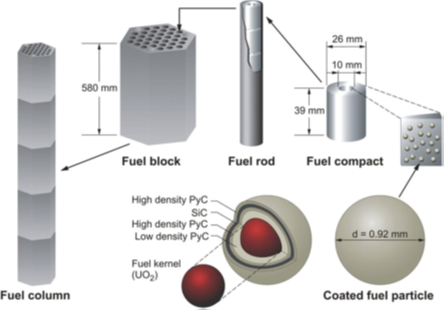
\includegraphics[width=0.6\textwidth]{figures/HTTR1.png}
        \caption{Fuel column loading of HTTR (obtained from \cite{bessEvaluationStartCore2009})}
        \label{fig:HTTR1}
\end{figure}

\begin{figure}[H]
        \centering
        \begin{subfigure}{.4\textwidth}
          \centering
          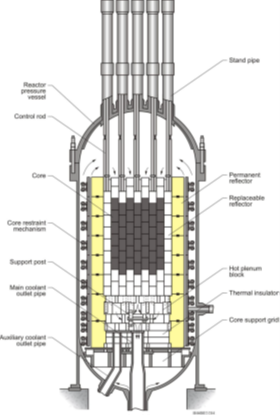
\includegraphics[width=\linewidth]{figures/HTTR2.png}
        \end{subfigure}
        \hfill
        \begin{subfigure}{.48\textwidth}
          \centering
          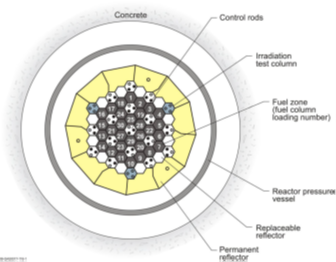
\includegraphics[width=\linewidth]{figures/HTTR3.png}
        \end{subfigure}
        \caption{Vertical (left) and horizontal (right) cross-sections of HTTR (obtained from \cite{bessEvaluationStartCore2009})}
        \label{fig:HTTR2}
\end{figure}

\begin{table}[H]
\centering
\caption{General parameters of HTTR}
\label{table:HTTRParam}

% Define custom color
\definecolor{myyellow}{RGB}{255, 255, 150}

\renewcommand{\arraystretch}{1.0} % row height

\begin{tabular}{|>{\raggedright\arraybackslash}p{8cm}|>{\centering\arraybackslash}m{3cm}|>{\centering\arraybackslash}m{3cm}|}
\hline
\rowcolor{myyellow}\multicolumn{3}{|c|}{\textbf{General Parameters}} \\ \hline
\centering\textbf{Parameter} & \textbf{Value} & \textbf{Unit} \\ \hline
Flat-to-flat core width & 436.48 & cm \\ \hline
Active core height (3D) & 522 & cm \\ \hline
Number of fuel block assembly & 30 & -- \\ \hline
Number of control block assembly & 19 & -- \\ \hline
Number of replaceable/permanent block assembly & 12/108 & -- \\ \hline

\rowcolor{myyellow}\multicolumn{3}{|c|}{\textbf{TRISO Kernels}} \\ \hline
Fuel kernel radius & 0.0300 & cm \\ \hline
Buffer layer outer radius & 0.0360 & cm \\ \hline
Inner PyC outer radius & 0.0390 & cm \\ \hline
SiC outer radius & 0.0415 & cm \\ \hline
Outer PyC radius & 0.0460 & cm \\ \hline
TRISO Packing Fraction & 30 & \% \\ \hline

\rowcolor{myyellow}\multicolumn{3}{|c|}{\textbf{Fuel Block Assembly}} \\ \hline
Fuel pin radius & 2.05 & cm \\ \hline
Coolant pin radius & 0.775 & cm \\ \hline
Burnable poison pin radius & 0.75 & cm \\ \hline
Number of fuel pins per block & 33 & -- \\ \hline
Number of burnable poison pins per block & 3 & -- \\ \hline
Fuel block height & 58 & cm \\ \hline
Flat-to-flat block width & 36 & cm \\ \hline
Fuel type & UO$_2$ & -- \\ \hline

\rowcolor{myyellow}\multicolumn{3}{|c|}{\textbf{Control Block Assembly}} \\ \hline
Control rod outer radius & 6.15 & cm \\ \hline
Control rod inner radius & 5.65 & cm \\ \hline

\rowcolor{myyellow}\multicolumn{3}{|c|}{\textbf{Coolant Block Assembly}} \\ \hline
Coolant pin radius & 1.15 & cm \\ \hline
Number of coolant pins per block & 33 & -- \\ \hline

\end{tabular}
\end{table}

For this dissertation, the design for HTTR startup core configuration with cold zero-power is used as the reference case. For the 2D case, not all variations of fuel enrichments are used. The 2D case is taken from the mid-plane block of the 3D case. The configuration map of the materials and fuel enrichment in the 2D case is shown in Figure \ref{fig:HTTR2Dconfig} \cite{bessEvaluationStartCore2009, zhangSimplifiedTwoThree2011}.

\begin{figure}[H]
        \centering
        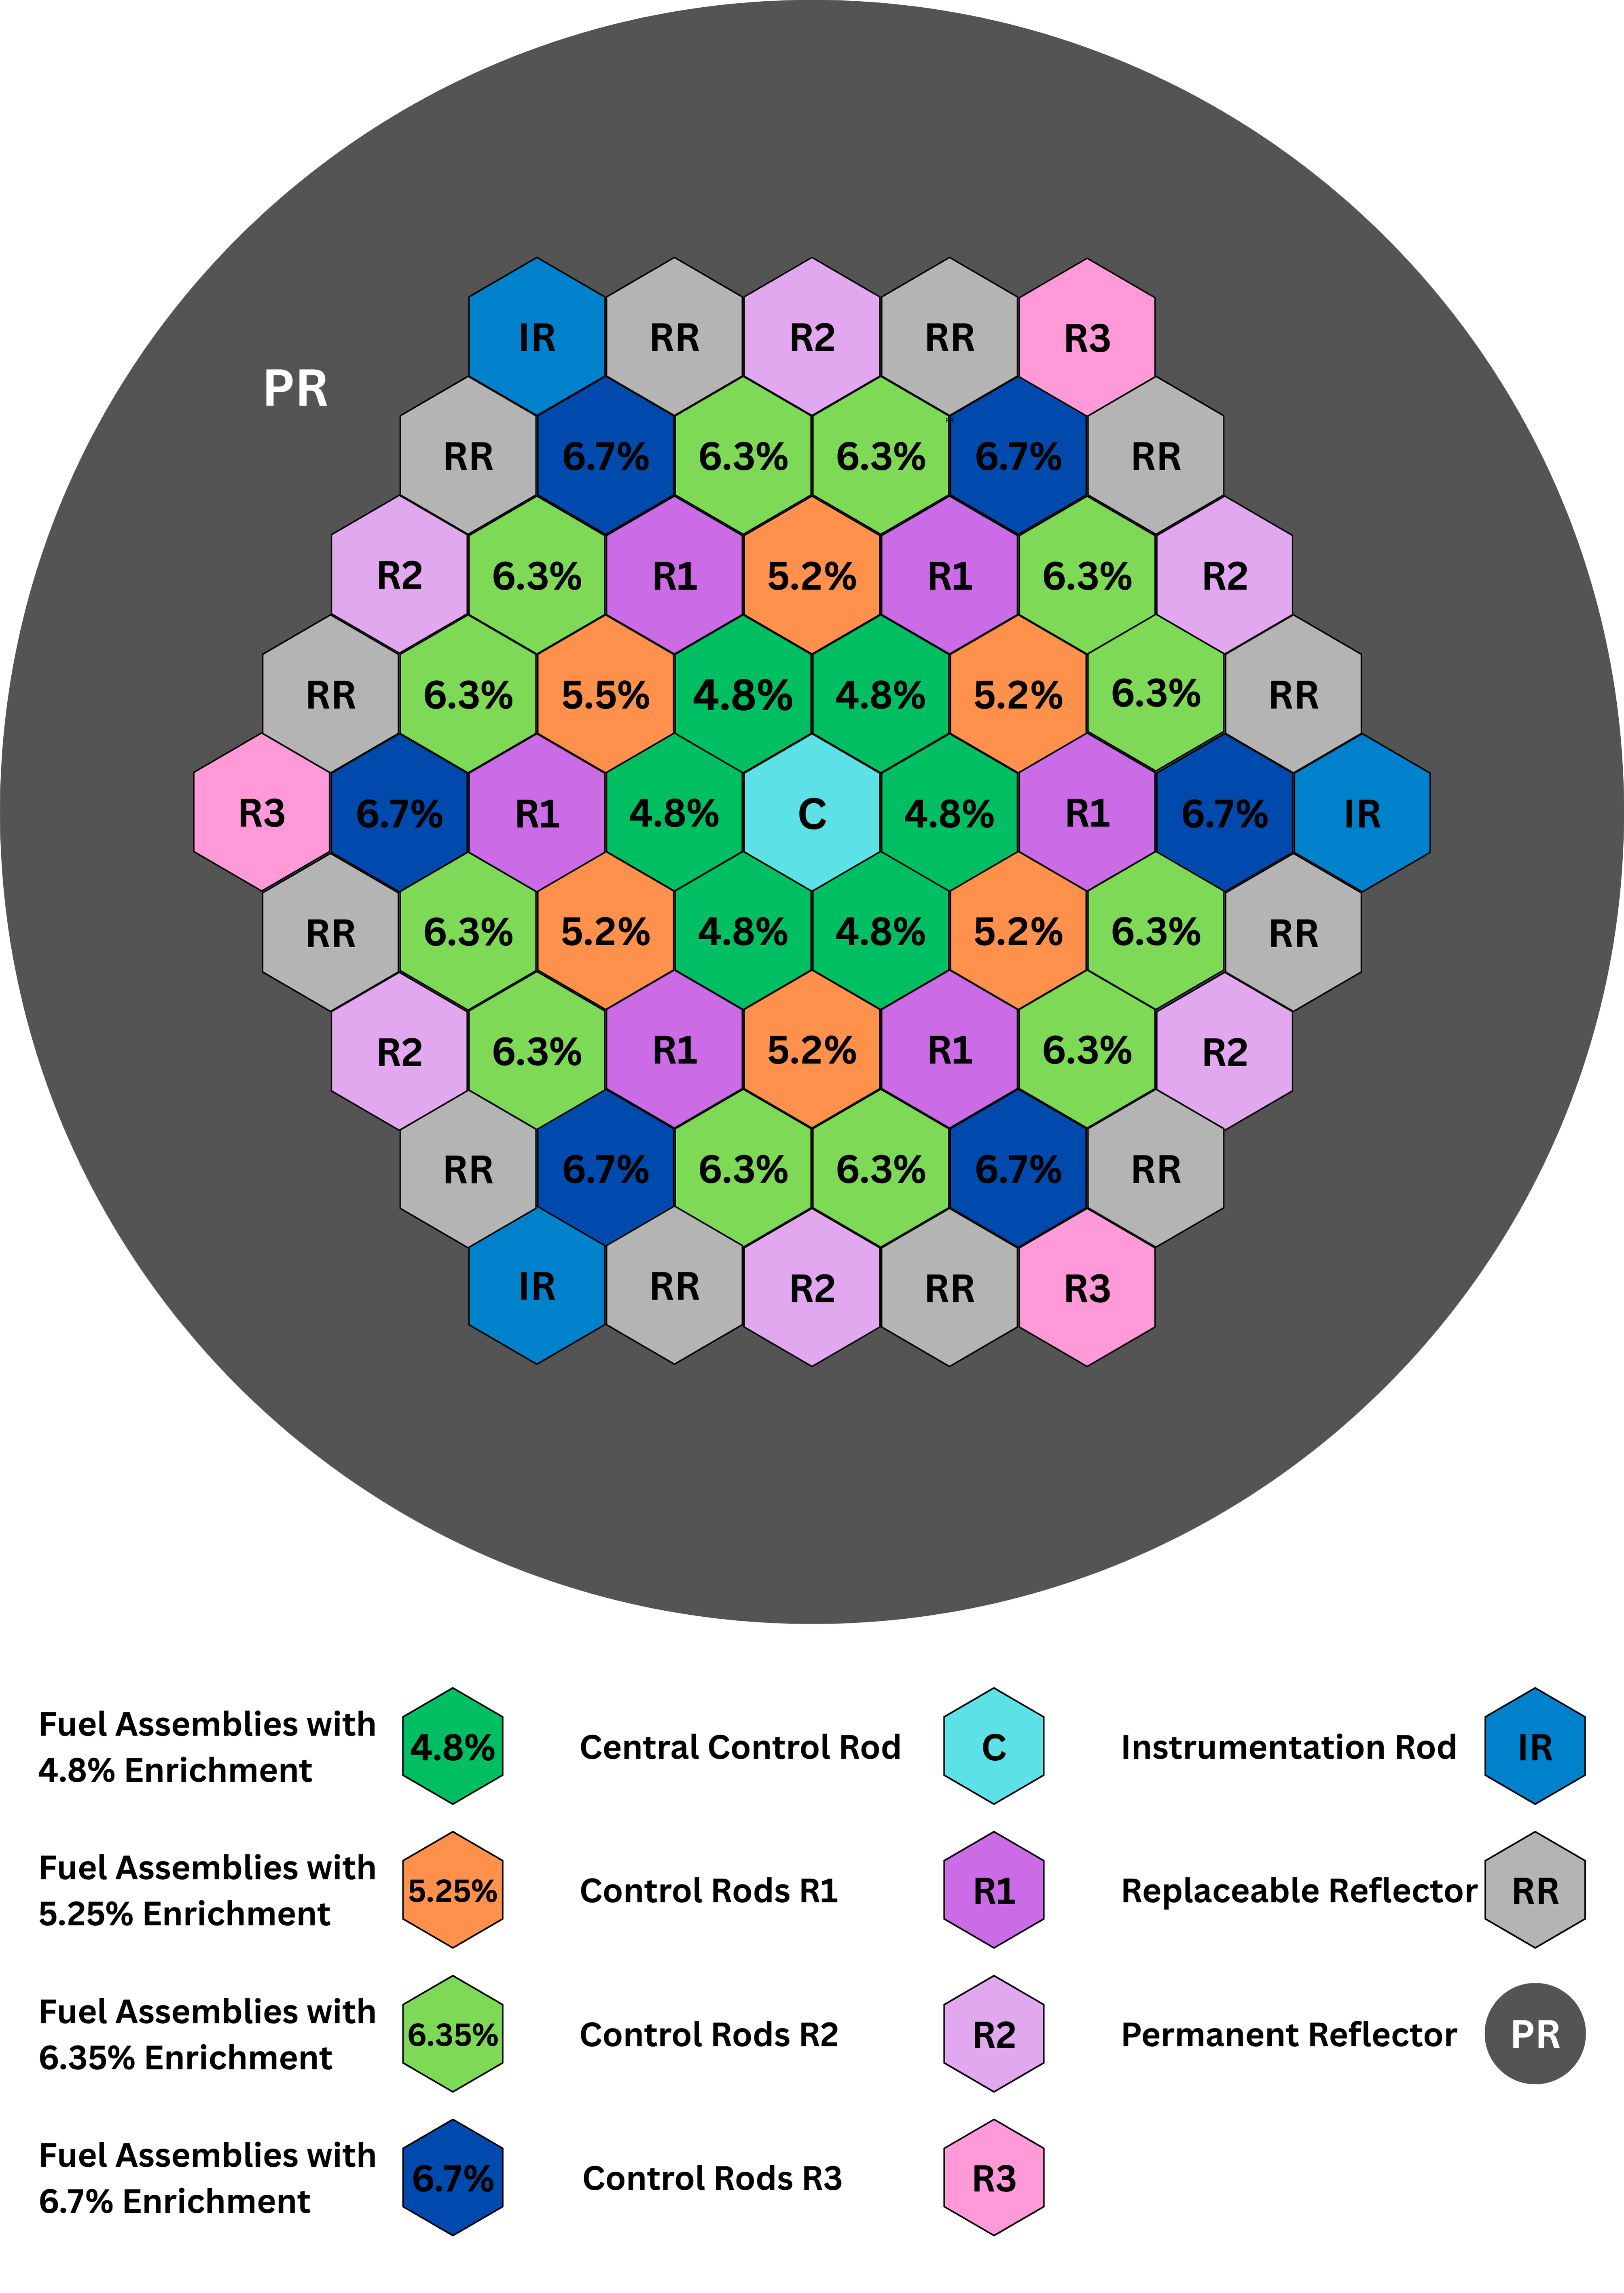
\includegraphics[width=0.45\textwidth]{figures/HTTR2Dconfig.png}
        \caption{Configuration map for 2D HTTR case}
        \label{fig:HTTR2Dconfig}
\end{figure}

For 3D case, the control rods are partially inserted to the level at which it is critical \cite{bessEvaluationStartCore2009, zhangSimplifiedTwoThree2011}. The configuration map of the 3D case in radial and axial directions is shown in Figure \ref{fig:HTTR3Dconfig} \cite{bessEvaluationStartCore2009, zhangSimplifiedTwoThree2011}.

\begin{figure}[H]
        \centering
        \begin{subfigure}{.48\textwidth}
          \centering
          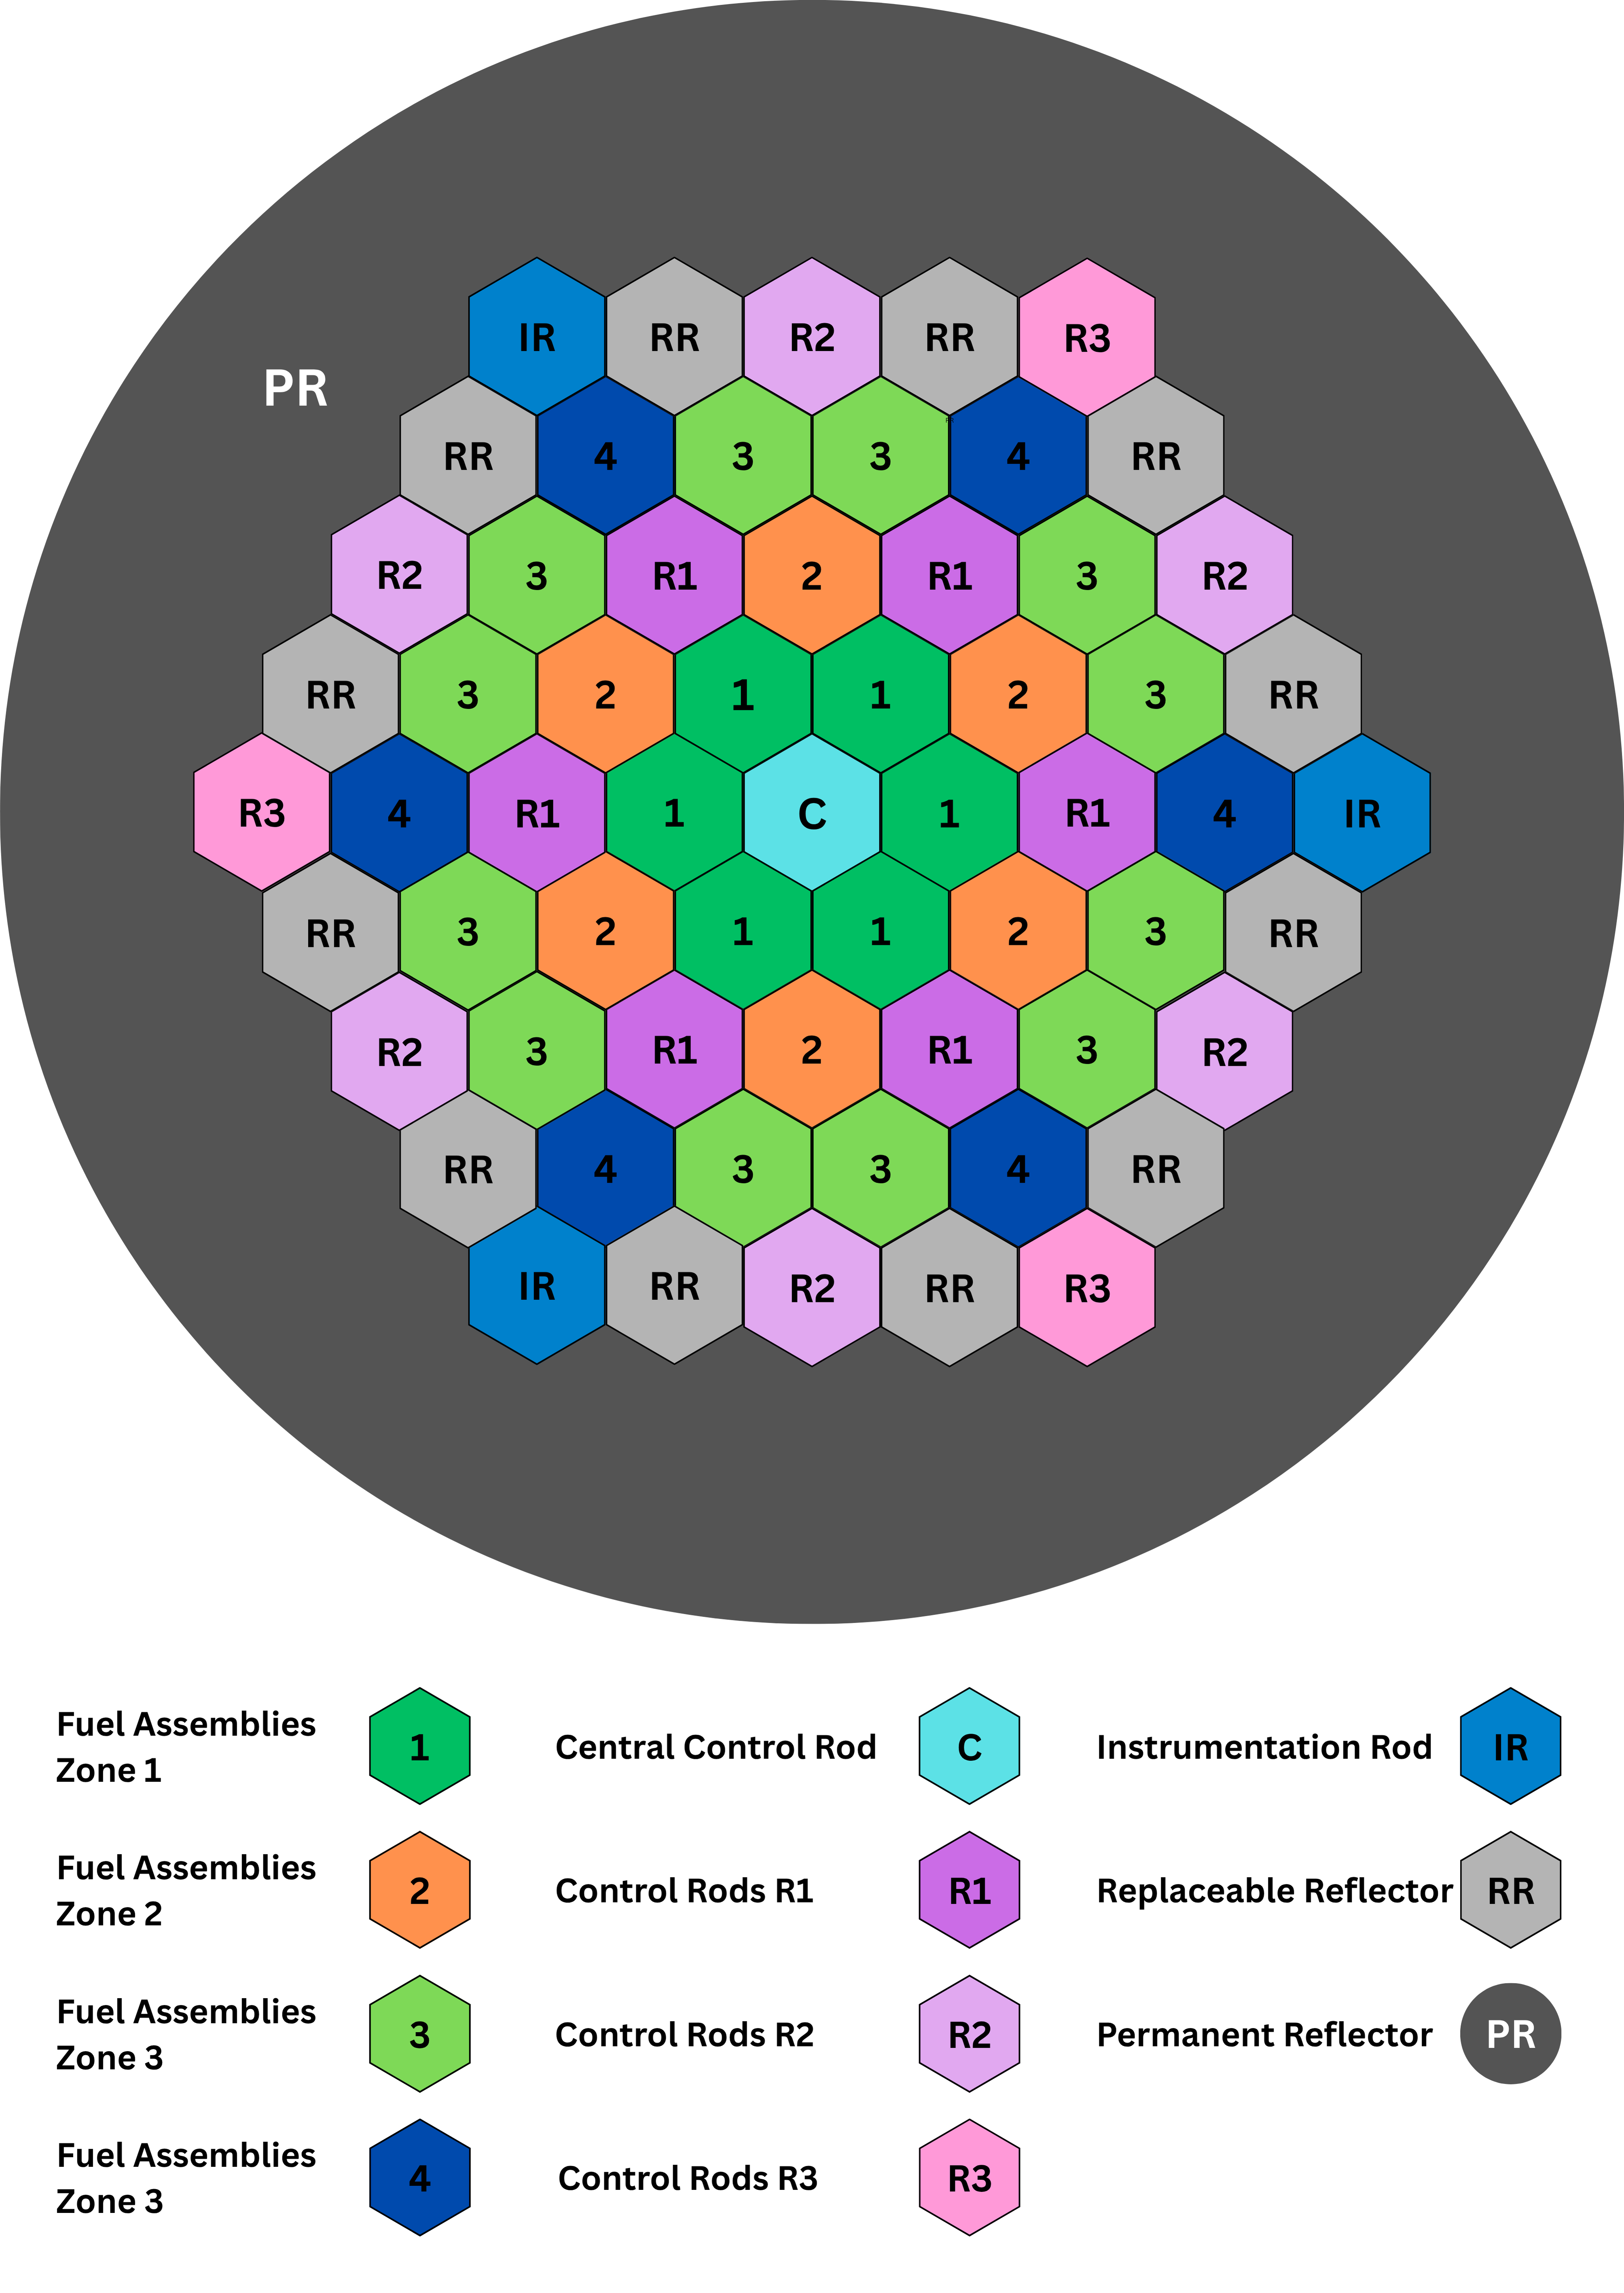
\includegraphics[width=\linewidth]{figures/HTTR3Dconfig1.png}
        \end{subfigure}
        \hfill
        \begin{subfigure}{.48\textwidth}
          \centering
          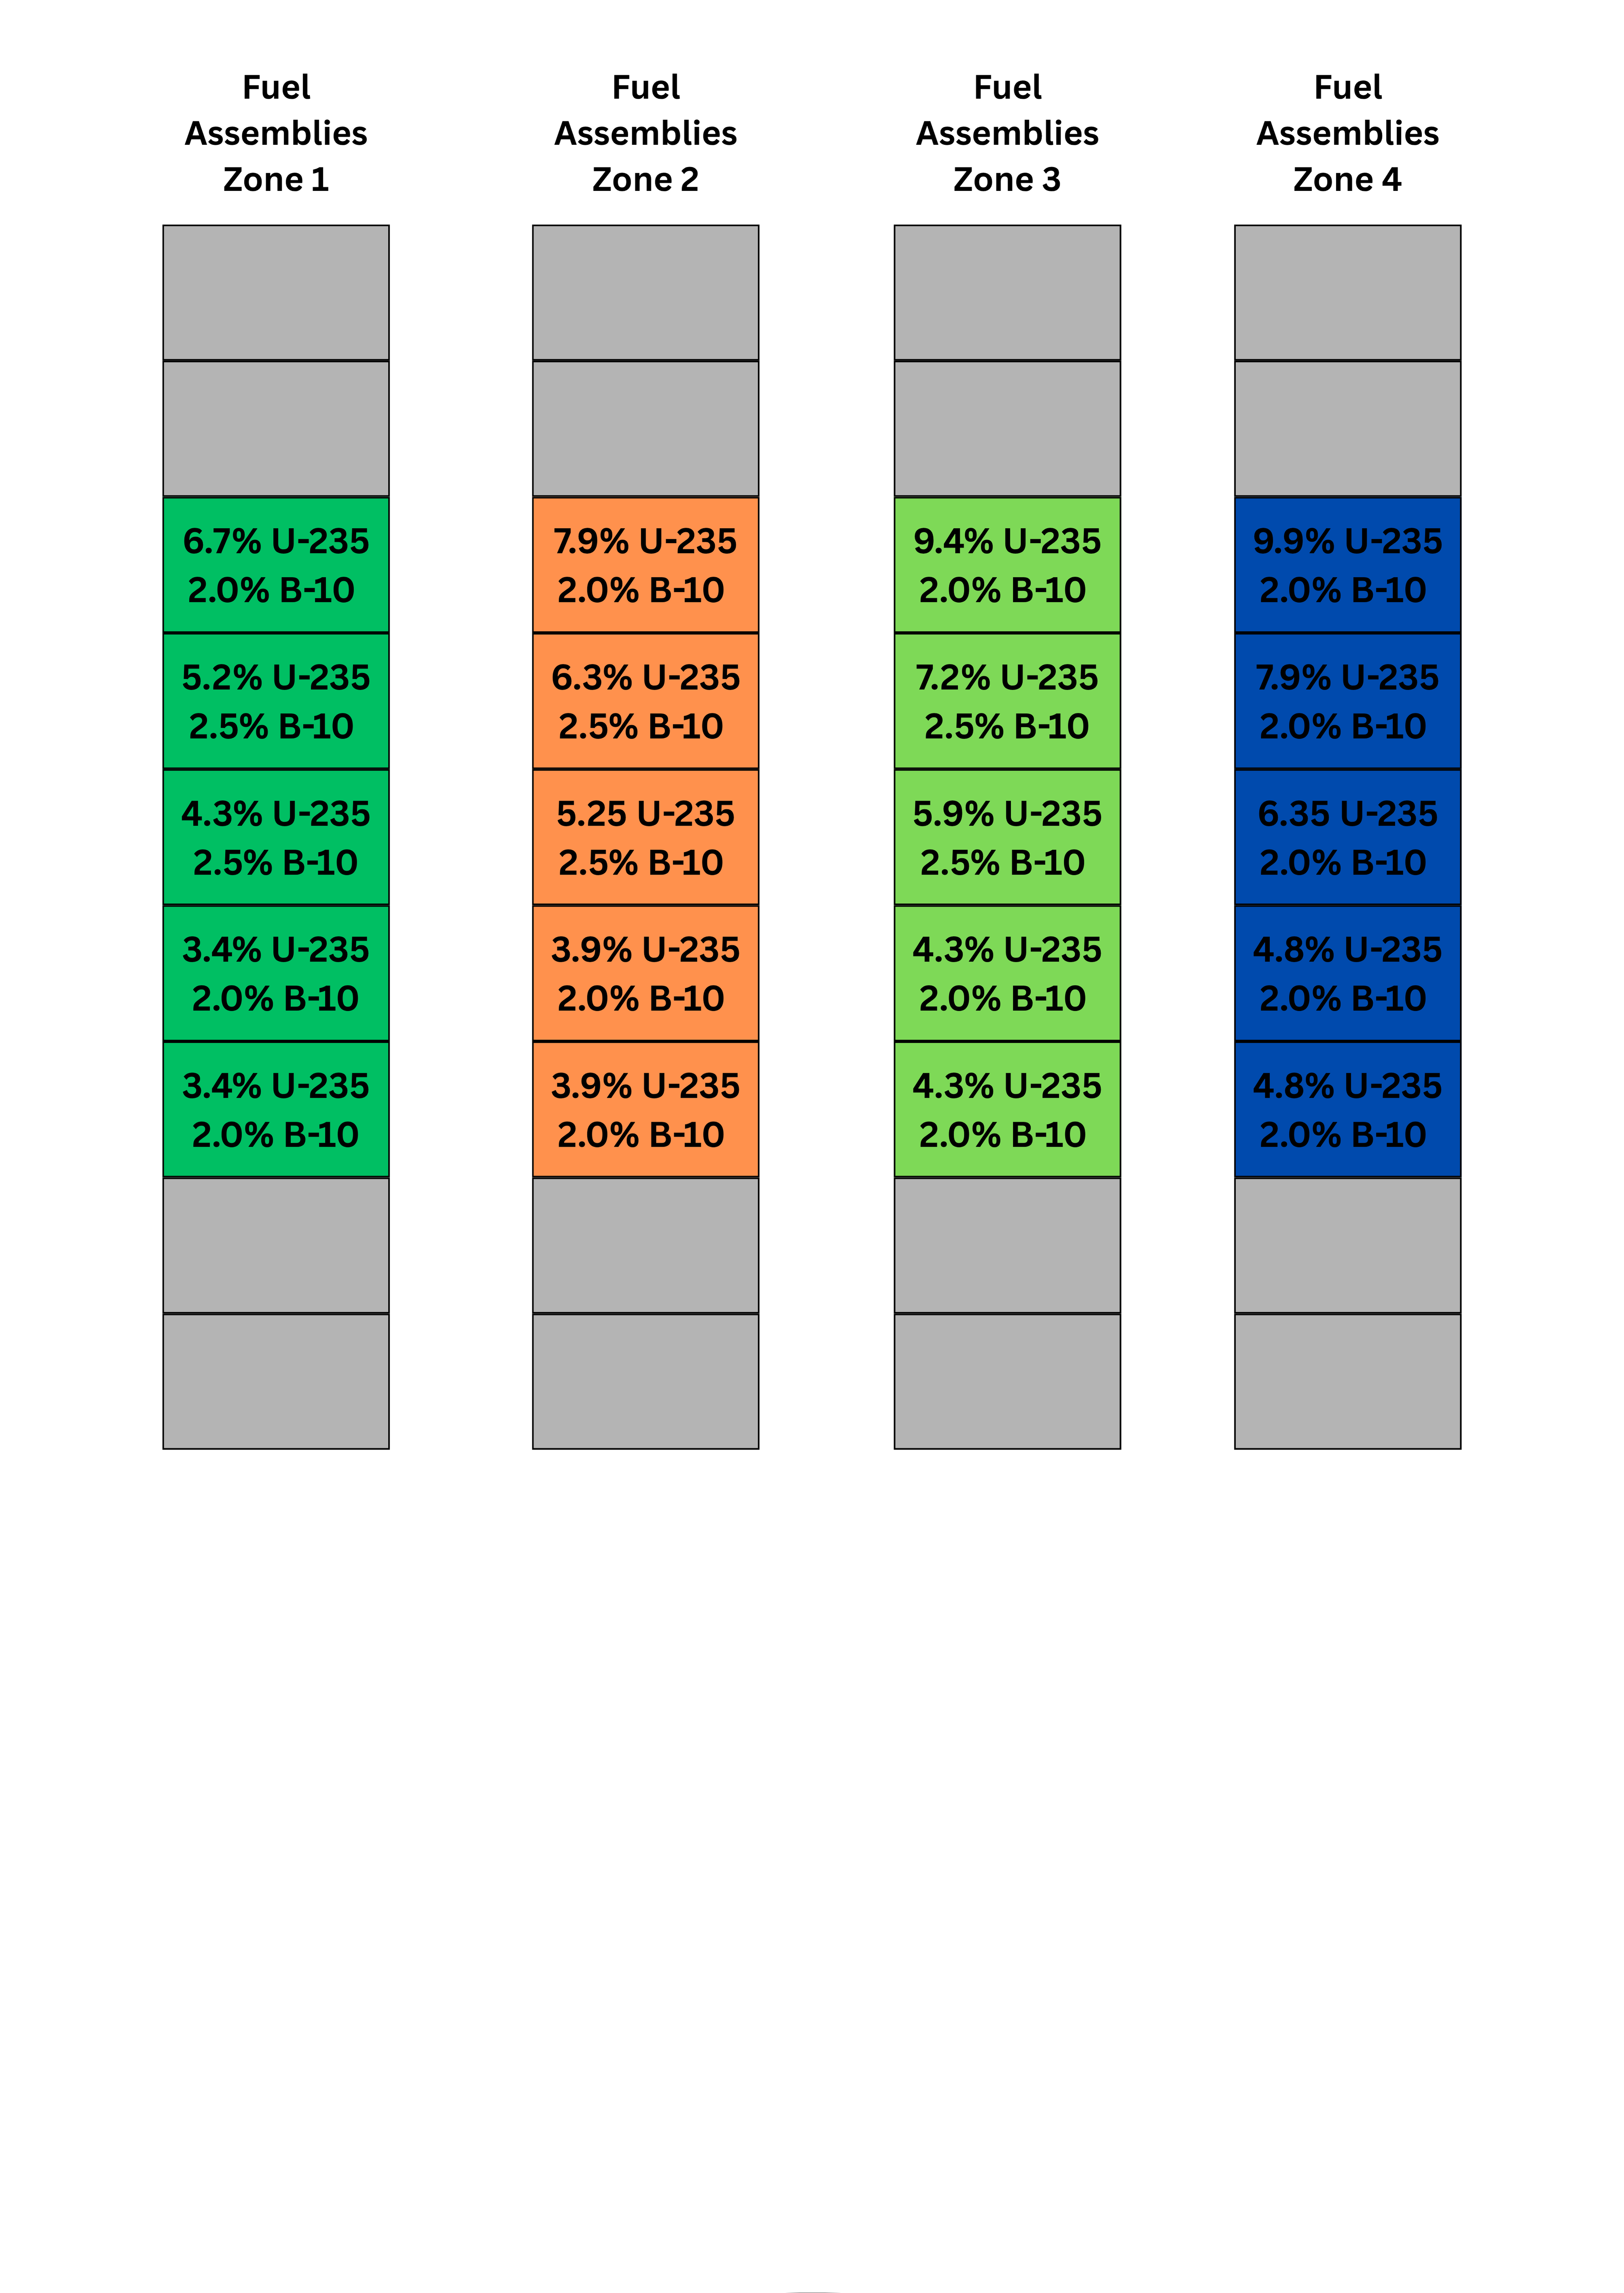
\includegraphics[width=\linewidth]{figures/HTTR3Dconfig2.png}
        \end{subfigure}
        \caption{Radial (left) and axial (right) configuration of 3D HTTR}
        \label{fig:HTTR3Dconfig}
\end{figure}

\section{Cross-section Homogenization using Serpent Monte Carlo Code}

The Serpent Monte Carlo code was developed by VTT Technical Research Center in Finland. It is a continuous-energy Monte Carlo particle code. Serpent has the capability to generate multigroup cross-sections for deterministic codes through spatial homogenization \cite{fridmanRevisedMethodsFewGroup2012, leppanenSerpentMonteCarlo2015}. Serpent has unique capabilities regarding the modeling of HTGRs. It has the capability to model the random TRISO distribution inside the fuel pellets. This modeling is done explicitly, in which the location of each TRISO fuel is generated using an automated disperser routine \cite{leppanenSerpentMonteCarlo2015}.

The spatial homogenization is used to preserve the local reaction balance when the group constants are generated from the solution of local heterogeneous transport. The homogenized, multigroup reaction cross-section $\Sigma_g$ is written as follows.
\begin{equation}
    \Sigma_g = \frac{\int_{E_g}^{E_{g-1}} dE \int_V dV \Sigma(\textbf{r}, E) \phi(\textbf{r}, E)}{\int_{E_g}^{E_{g-1}} dE \int_V dV \phi(\textbf{r}, E)}
\end{equation}
where $\phi(\textbf{r}, E)$ is the scalar flux. The integration is performed over the volume of the homogenized region and energy group. One of the advantages of using Monte Carlo simulations for cross-section homogenization is that the stochastic estimates of the integral values of the reaction rates and the integral value of the flux over space and energy can be obtained directly from the simulation \cite{leppanenOverviewMethodologySpatial2016}.

For this dissertation, homogenized cross-sections are generated for each block in the core, which is defined as a distinct universe. For the 2D core, 128 universes are defined, and for the 3D core, 1144 universes are defined. Each universe generates homogenized cross-sections that will be post-processed and used as inputs to the neutron noise simulation tool.

\section{Forward Simulation of HTTR}

\subsection{2D Forward Flux}

In this simulation, the solution for the developed tool is compared to the Serpent Monte Carlo results. The output of Serpent is assembly-averaged flux distribution, which is then normalized in the postprocess. For the developed tool, the output is the flux distribution for triangular mesh. In this case, each hexagon is divided into six triangles. To obtain the assembly-averaged flux distribution, we performed the following:
\begin{equation}
    \phi_{g,k} = \frac{\sum_{i=1}^I \phi_{g,i}}{V_k}
\end{equation}
where,
\begin{itemize}
    \item[] $\phi_{g,i}$ = Neutron flux for group $g$ and triangle $i$,
    \item[] $I$ = = Total number of triangles in every assembly, 
    \item[] $\phi_{g,k}$ = Neutron flux for group $g$ and assembly $k$, 
    \item[] $V_k$ = Volume of assembly $k$. 
\end{itemize}

The relative error is calculated as follows:
\begin{equation}\label{eq:error_serpent}
    \varepsilon_k = \frac{|\phi_{k,\text{calc}}-\phi_{k,\text{serpent}}|}{|\phi_{k,\text{serpent}}|}
\end{equation}
The results for these calculations are as follows:
\begin{table}[H]
        \centering
        \caption{Eigenvalue comparison of 2D HTTR}
        \label{table:2DHTTR_fw_results}
        \begin{tabular}{ | M{3.5cm} | M{4cm} | } 
         \hline
         $k_{\text{eff}}$ Serpent & 0.991938 $\pm$ 0.00012  \\
         \hline
         $k_{\text{eff}}$ Tool & 1.002590  \\
         \hline
         Absolute Error (pcm) & 1065.2  \\
         \hline
        \end{tabular}
\end{table}

\begin{figure}[H]
        \centering
        \begin{subfigure}{.48\textwidth}
          \centering
          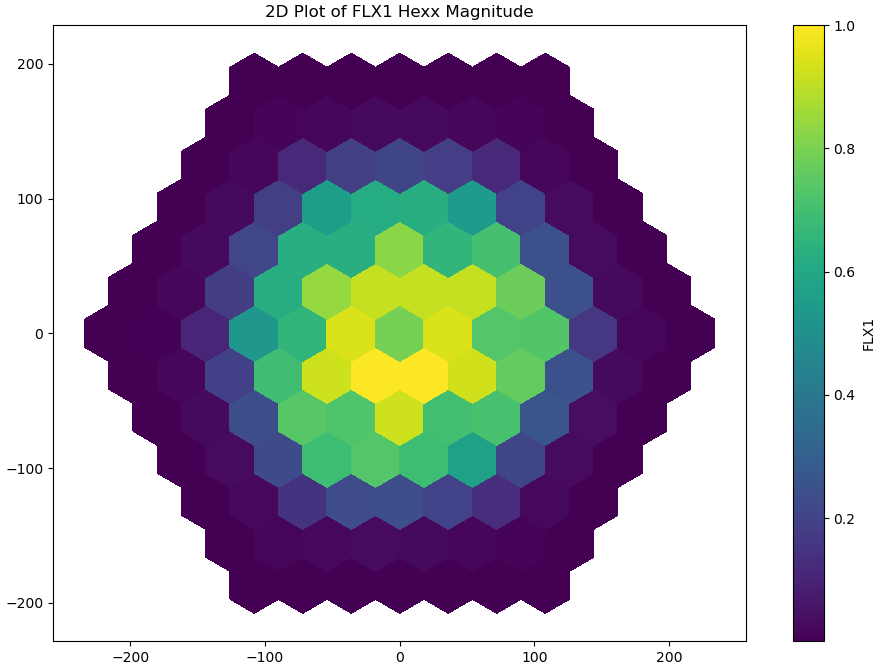
\includegraphics[width=\linewidth]{figures/OBJECTIVES1_TEST08_2DTriMG_HTTR2G_VandV_level1_FORWARD_FLX_magnitude_G1.png}
        \end{subfigure}
        \hfill
        \begin{subfigure}{.48\textwidth}
          \centering
          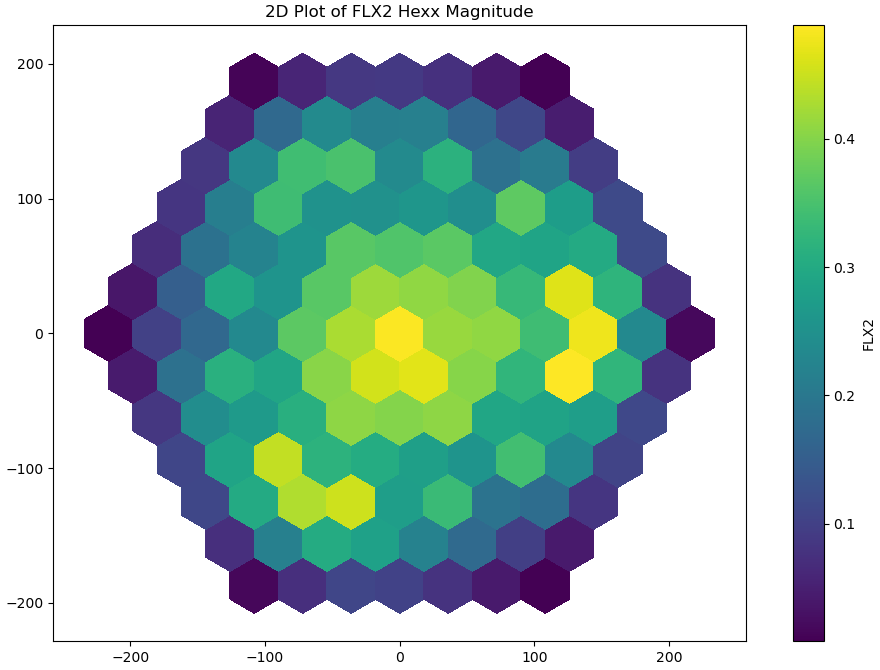
\includegraphics[width=\linewidth]{figures/OBJECTIVES1_TEST08_2DTriMG_HTTR2G_VandV_level1_FORWARD_FLX_magnitude_G2.png}
        \end{subfigure}
        \caption{Forward flux results from Serpent}
        \label{fig:2DHTTR_fw_results_flx}
\end{figure}
\begin{figure}[H]
        \centering
        \begin{subfigure}{.48\textwidth}
          \centering
          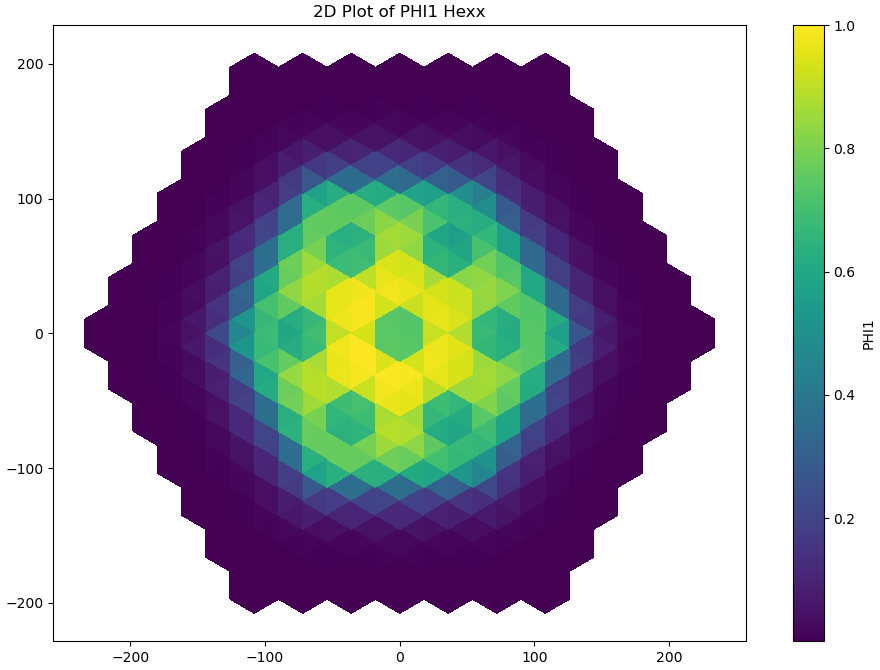
\includegraphics[width=\linewidth]{figures/OBJECTIVES1_TEST08_2DTriMG_HTTR2G_VandV_level1_FORWARD_PHI_magnitude_G1.png}
        \end{subfigure}
        \hfill
        \begin{subfigure}{.48\textwidth}
          \centering
          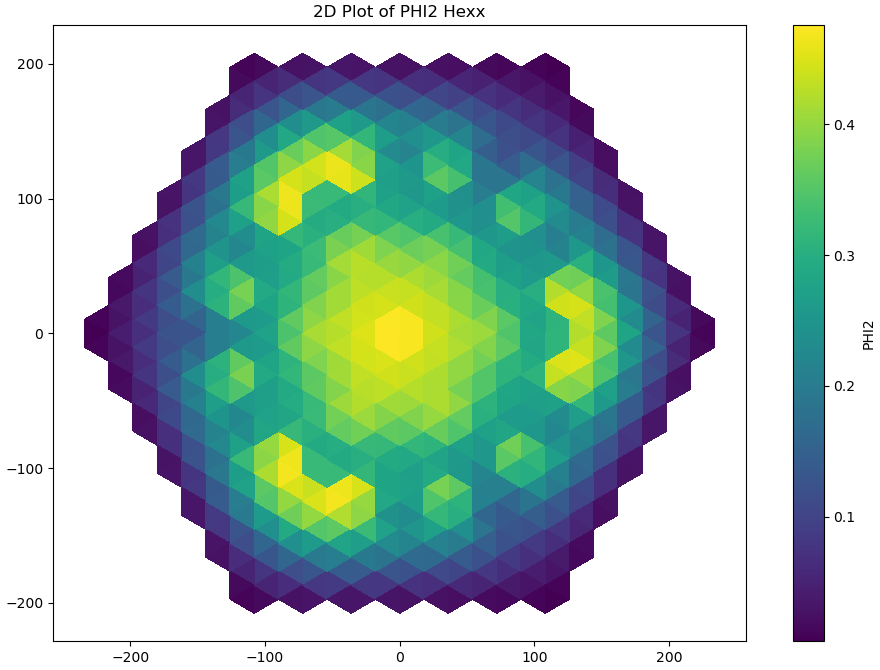
\includegraphics[width=\linewidth]{figures/OBJECTIVES1_TEST08_2DTriMG_HTTR2G_VandV_level1_FORWARD_PHI_magnitude_G2.png}
        \end{subfigure}
        \caption{Forward flux results from the developed tool}
        \label{fig:2DHTTR_fw_results_phi}
\end{figure}
\begin{figure}[H]
        \centering
        \begin{subfigure}{.48\textwidth}
          \centering
          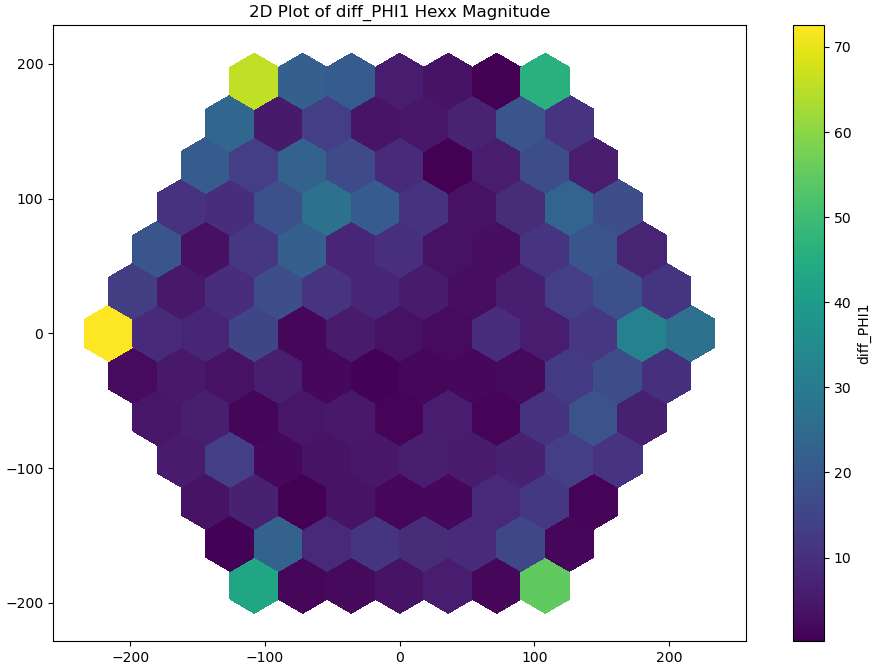
\includegraphics[width=\linewidth]{figures/OBJECTIVES1_TEST08_2DTriMG_HTTR2G_VandV_level1_FORWARD_diff_PHI_magnitude_G1.png}
        \end{subfigure}
        \hfill
        \begin{subfigure}{.48\textwidth}
          \centering
          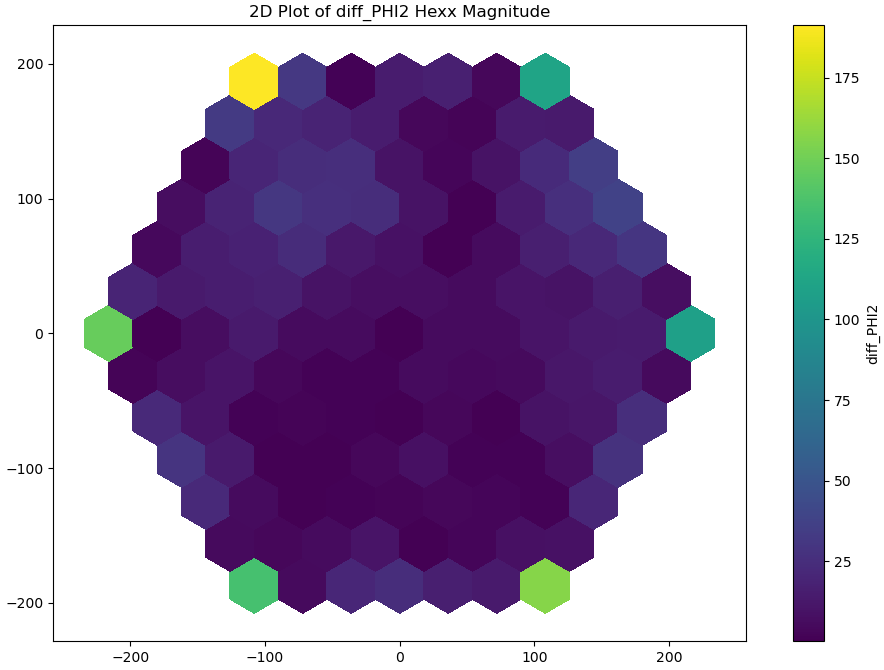
\includegraphics[width=\linewidth]{figures/OBJECTIVES1_TEST08_2DTriMG_HTTR2G_VandV_level1_FORWARD_diff_PHI_magnitude_G2.png}
        \end{subfigure}
        \caption{Difference of forward flux between Serpent and the tool}
        \label{fig:2DHTTR_fw_results_diff_phi}
\end{figure}

The results from Table \ref{table:2DHTTR_fw_results}, Figure \ref{fig:2DHTTR_fw_results_flx}, Figure \ref{fig:2DHTTR_fw_results_phi}, and Figure \ref{fig:2DHTTR_fw_results_diff_phi} show that, in general, the forward flux results obtained from the developed tool are in good agreement with the Serpent results. For the eigenvalue results, the difference in $k_{\text{eff}}$ is expected due to the homogenization of macroscopic cross-sections that are used in the developed tool. The heterogeneity effect of the HTTR is suppressed due to the spatial homogenization of the cross-sections. Also, the neutron diffusion method underestimates the neutron leakage due to its assumption of linear anisotropy. The flux differences are mainly in the periphery of the core. This behavior is expected, as the peripheral regions are filled with reflector materials, where the neutron flux is relatively low. 

\subsection{3D Forward Flux}

For the 3D forward flux simulation, the solution for the developed tool is compared to the Serpent Monte Carlo results. The output of Serpent is assembly-averaged flux distribution, which is then normalized in the postprocess. The assembly in this case is defined as a fuel block with a height of 58 cm. For the developed tool, the output is the flux distribution for each triangular prism. In this case, each hexagonal prism is divided into six triangular prisms. The error used in this case is defined in Eq. \ref{eq:error_serpent}. 

The results for these calculations are as follows:
\begin{table}[H]
        \centering
        \caption{Eigenvalue comparison of 3D HTTR}
        \label{table:3DHTTR_fw_results}
        \begin{tabular}{ | M{3.5cm} | M{4cm} | } 
         \hline
         $k_{\text{eff}}$ Serpent & 1.021540 $\pm$ 0.000094  \\
         \hline
         $k_{\text{eff}}$ Tool & 1.050390  \\
         \hline
         Absolute Error (pcm) & -2885.0  \\
         \hline
        \end{tabular}
\end{table}

\begin{figure}[H]
        \centering
        \begin{subfigure}{.48\textwidth}
          \centering
          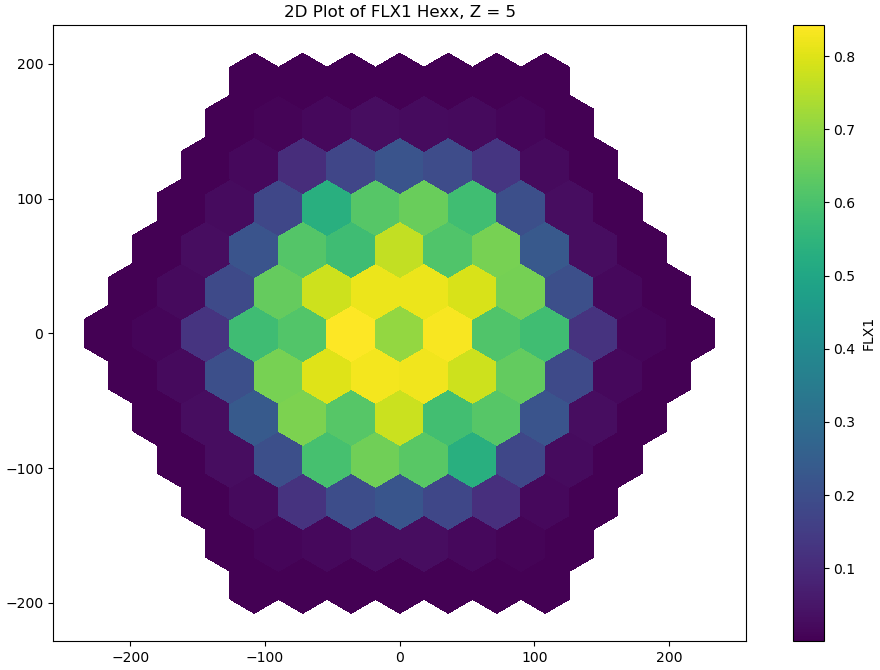
\includegraphics[width=\linewidth]{figures/OBJECTIVES1_TEST09_3DTriMG_HTTR_level1_FORWARD_FLX_magnitude_G1_Z5.png}
        \end{subfigure}
        \hfill
        \begin{subfigure}{.48\textwidth}
          \centering
          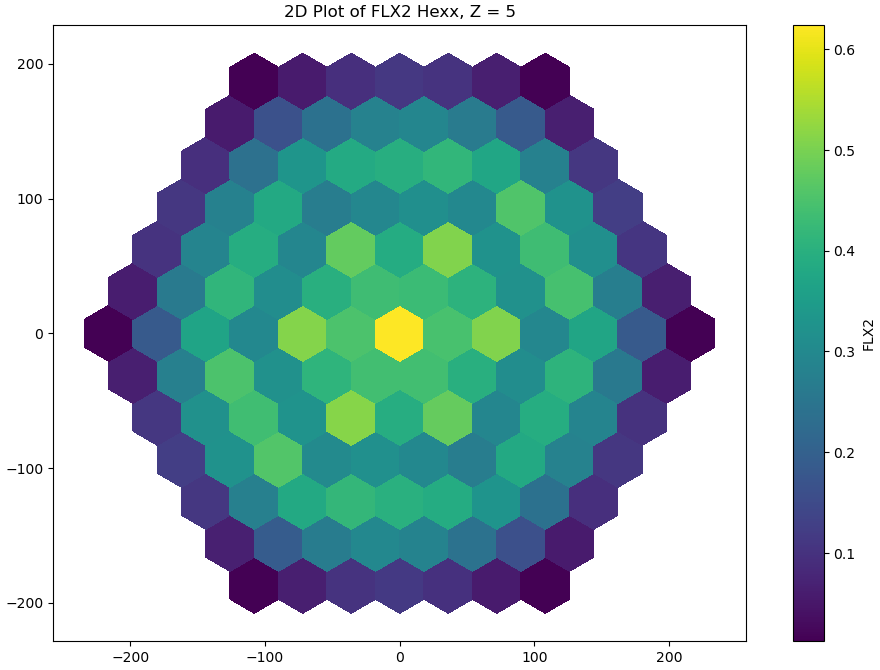
\includegraphics[width=\linewidth]{figures/OBJECTIVES1_TEST09_3DTriMG_HTTR_level1_FORWARD_FLX_magnitude_G2_Z5.png}
        \end{subfigure}
        \caption{Forward flux of 3D HTTR at midplane ($Z=5$) from Serpent}
        \label{fig:3DHTTR_fw_results_flx}
\end{figure}
\begin{figure}[H]
        \centering
        \begin{subfigure}{.48\textwidth}
          \centering
          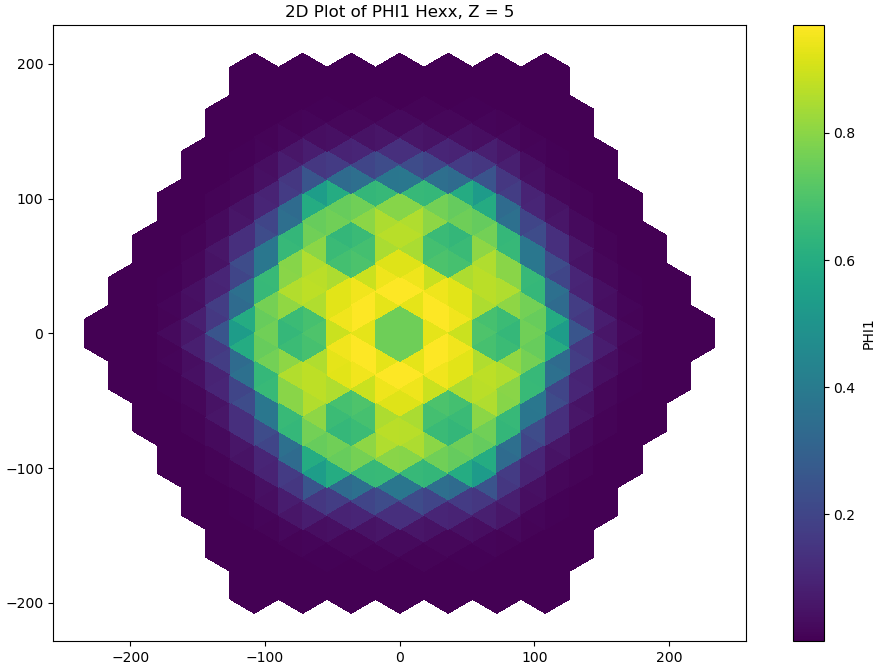
\includegraphics[width=\linewidth]{figures/OBJECTIVES1_TEST09_3DTriMG_HTTR_level1_FORWARD_PHI_magnitude_G1_Z5.png}
        \end{subfigure}
        \hfill
        \begin{subfigure}{.48\textwidth}
          \centering
          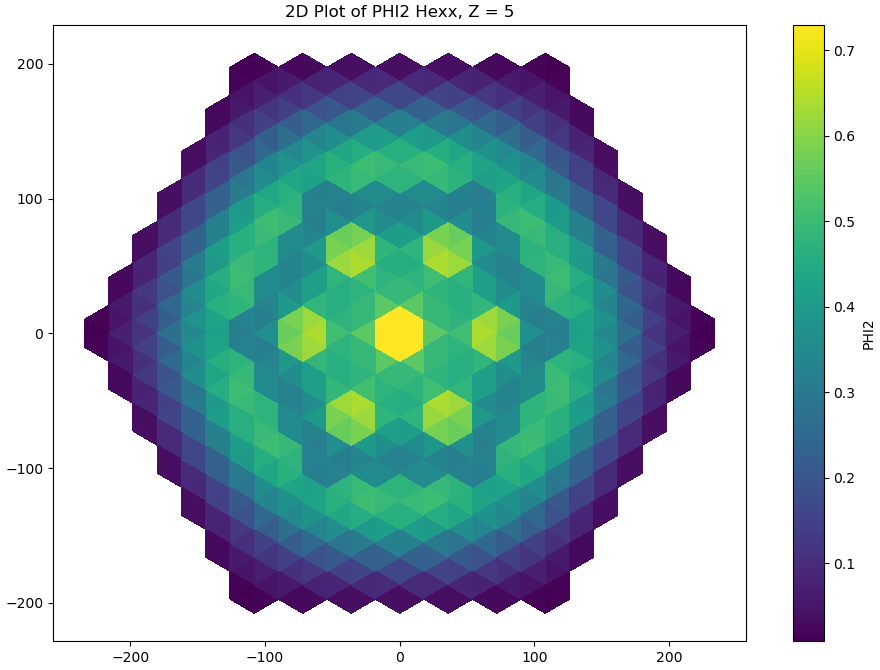
\includegraphics[width=\linewidth]{figures/OBJECTIVES1_TEST09_3DTriMG_HTTR_level1_FORWARD_PHI_magnitude_G2_Z5.png}
        \end{subfigure}
        \caption{Forward flux of 3D HTTR at midplane ($Z=5$) from the developed tool}
        \label{fig:3DHTTR_fw_results_phi}
\end{figure}
\begin{figure}[H]
        \centering
        \begin{subfigure}{.48\textwidth}
          \centering
          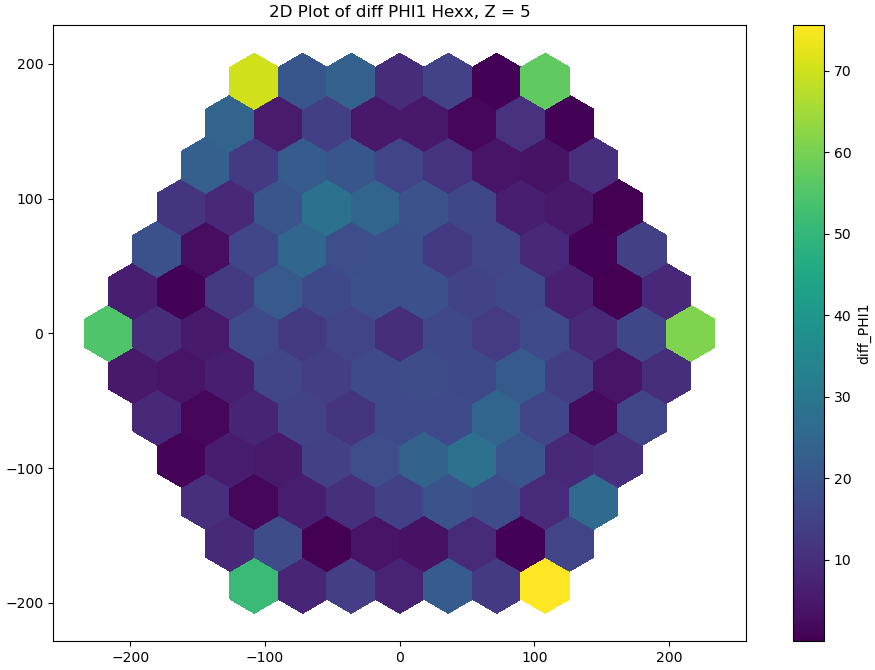
\includegraphics[width=\linewidth]{figures/OBJECTIVES1_TEST09_3DTriMG_HTTR_level1_FORWARD_diff_PHI_magnitude_G1_Z5.png}
        \end{subfigure}
        \hfill
        \begin{subfigure}{.48\textwidth}
          \centering
          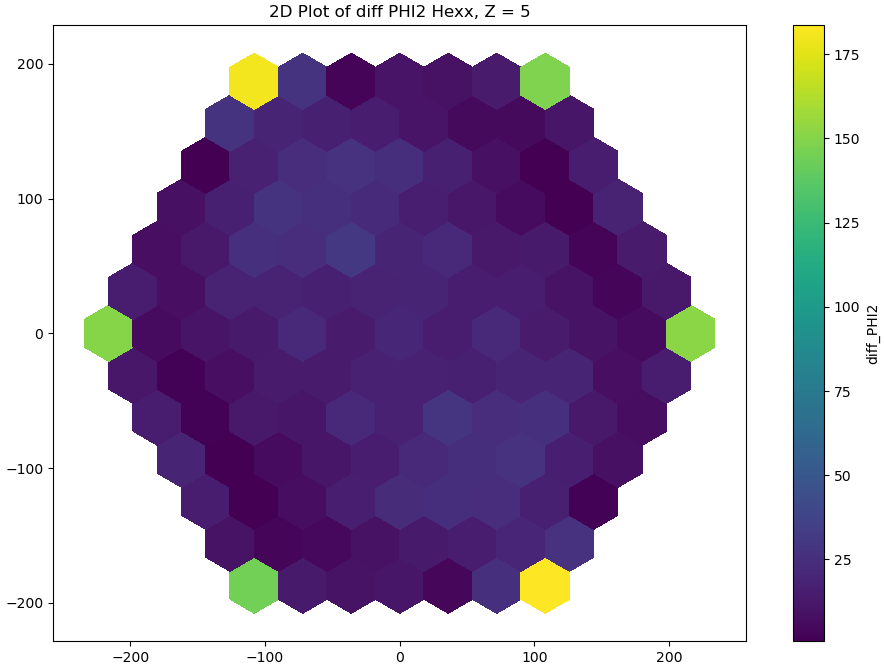
\includegraphics[width=\linewidth]{figures/OBJECTIVES1_TEST09_3DTriMG_HTTR_level1_FORWARD_diff_PHI_magnitude_G2_Z5.png}
        \end{subfigure}
        \caption{Difference of forward flux between Serpent and the developed tool}
        \label{fig:3DHTTR_fw_results_diff_phi}
\end{figure}

The results from Table \ref{table:3DHTTR_fw_results}, Figure \ref{fig:3DHTTR_fw_results_flx}, Figure \ref{fig:3DHTTR_fw_results_phi}, and Figure \ref{fig:3DHTTR_fw_results_diff_phi} show that, in general, the forward flux results obtained from the developed tool are in good agreement with the Serpent results. Overall, it shows similar observations compared to the 2D HTTR system. The difference in $k_{\text{eff}}$ is mainly due to the homogenization of macroscopic cross-sections and the assumption of neutron diffusion theory. The flux differences are primarily in the periphery of the core. This behavior is expected, as the peripheral regions are filled with reflector materials, where the neutron flux is relatively low. 

\section{Neutron Noise Simulation of HTTR}

\subsection{2D HTTR with Absorber of Variable Strength Source}

For this simulation, the neutron noise source is defined as a perturbation of the thermal absorption cross-section in the fuel assembly. The perturbation can be written as follows:
\begin{equation}
    \delta \Sigma_{a,2}(\textbf{r}, \omega) = \gamma(\omega) \delta(\textbf{r} - \textbf{r}_0)
\end{equation}
where $\gamma(\omega)$ is defined as 5\% of the thermal absorption cross-section at $r_0$ and $r_0$ is defined as one mesh in assembly number 65 (indicated as red triangle), which is shown in Figure \ref{fig:HTTR2DAVS}.
\begin{figure}[H]
        \centering
        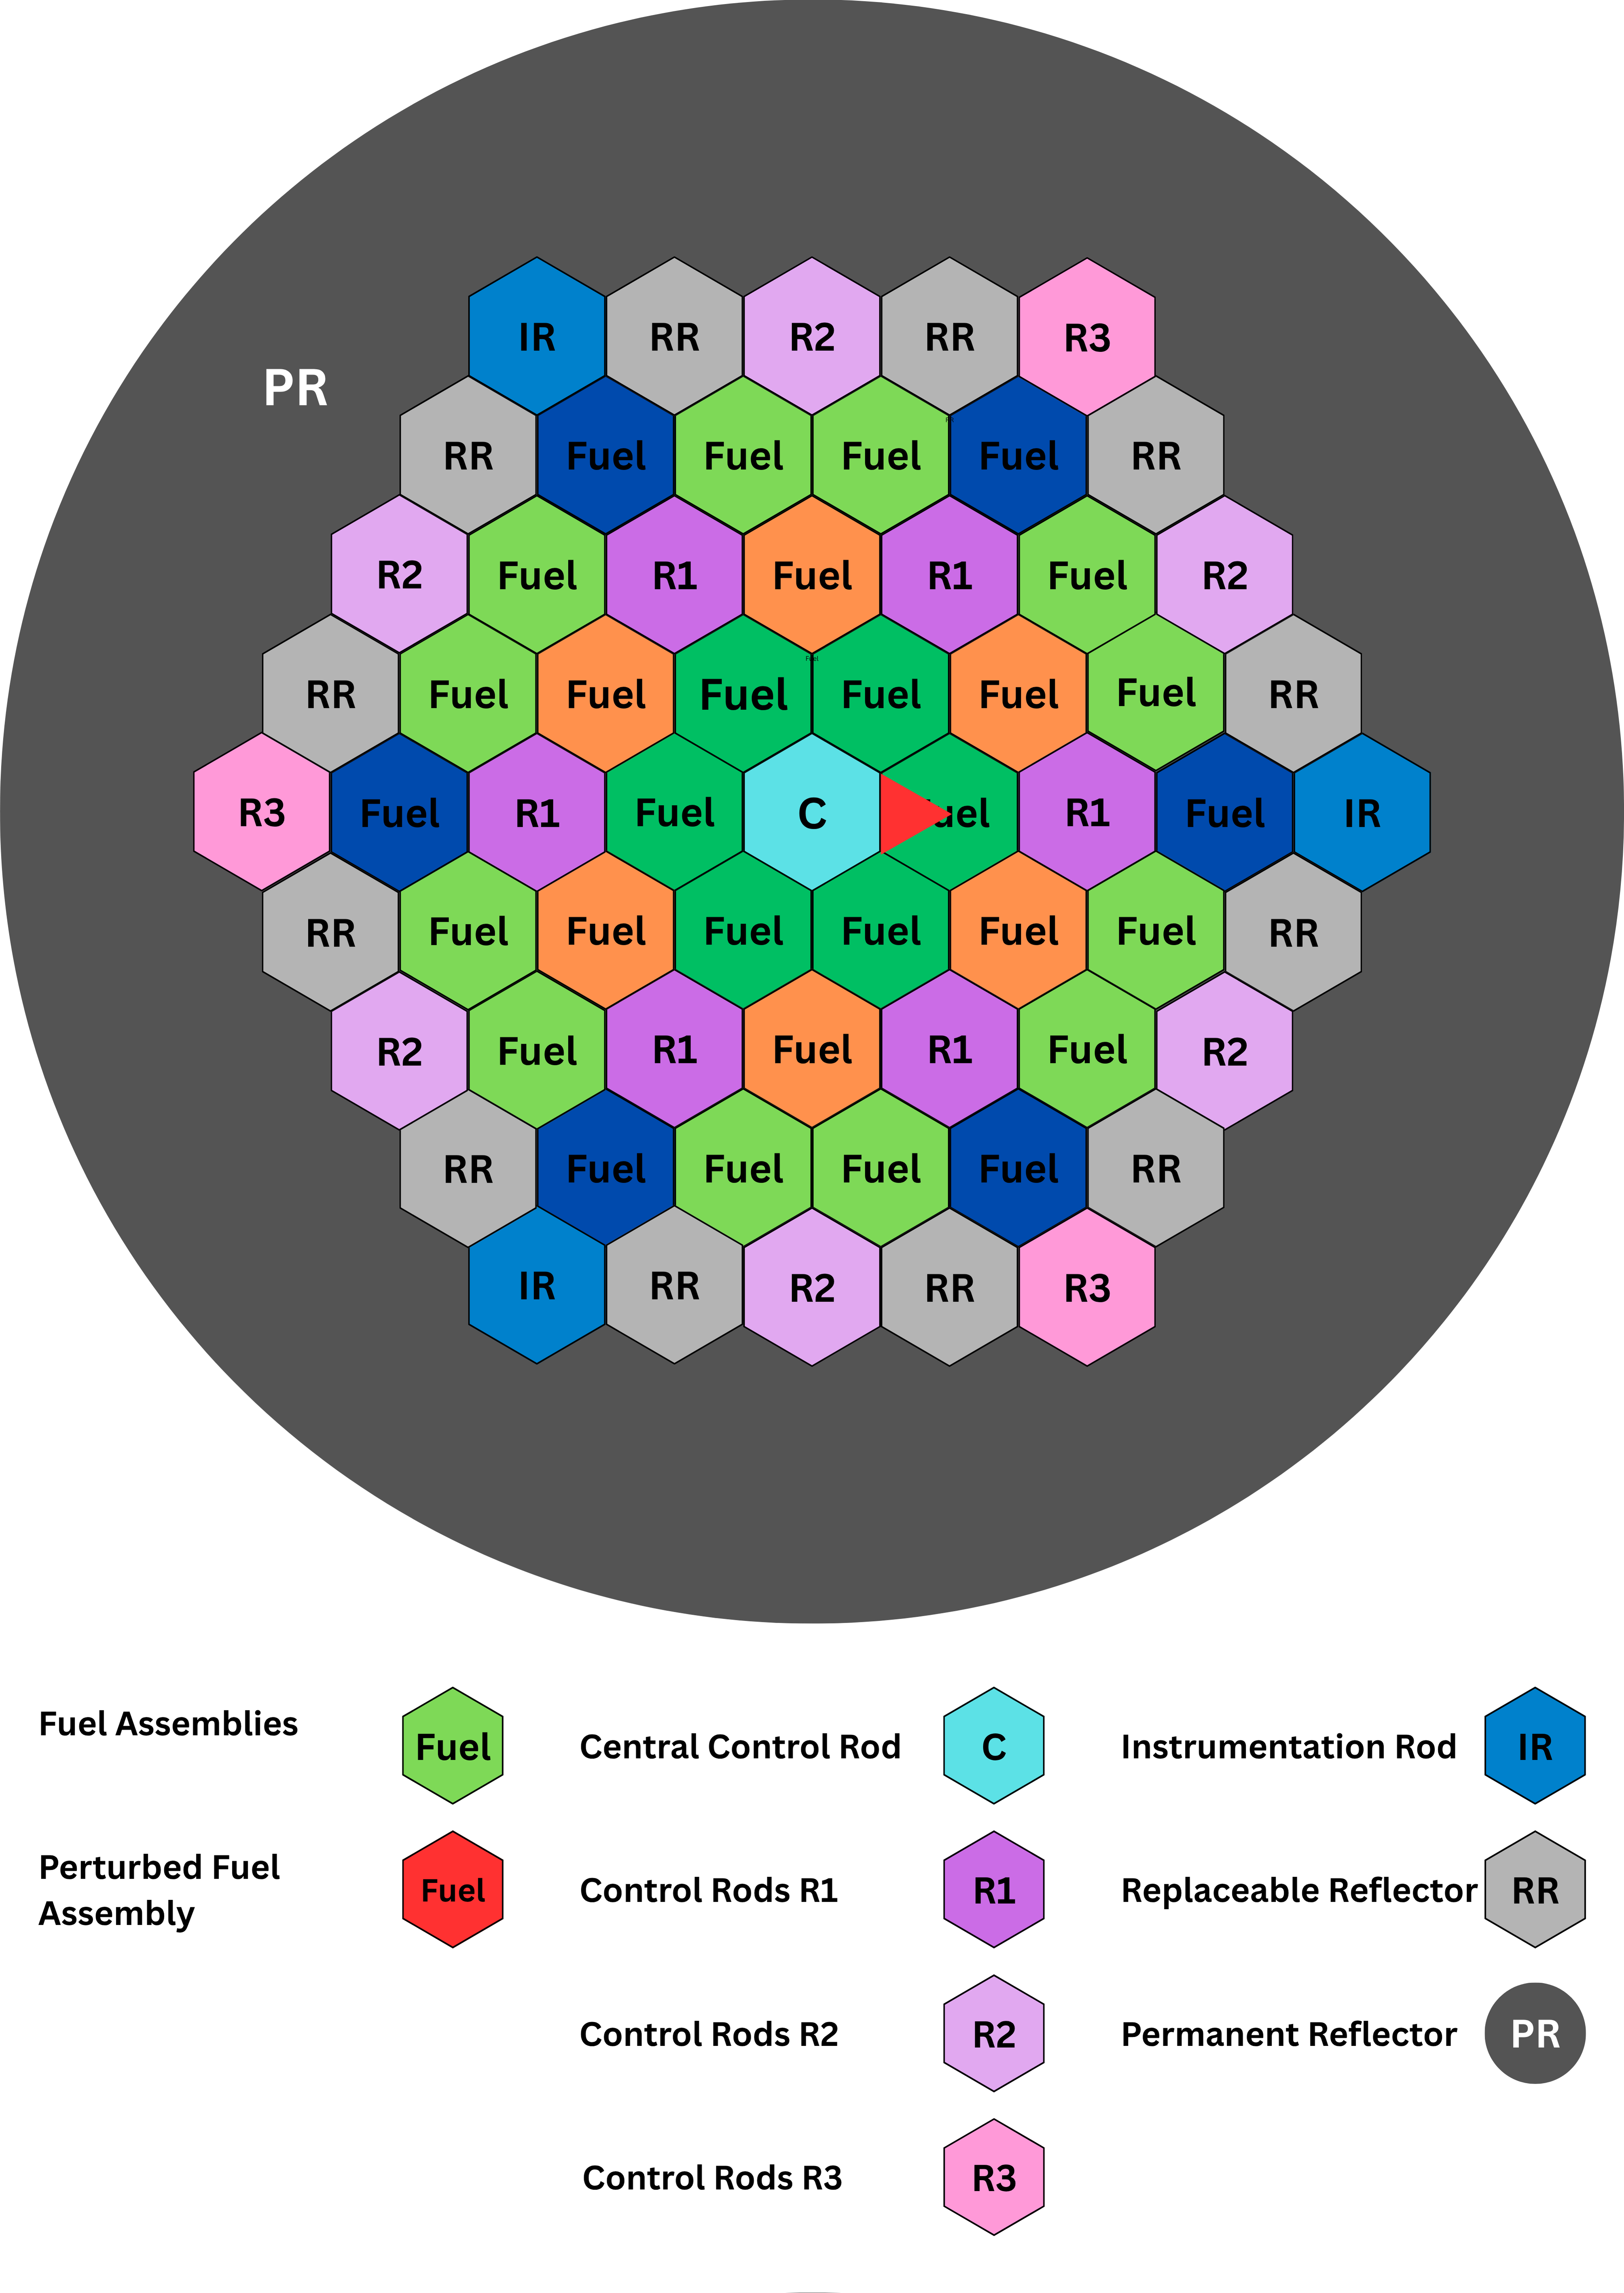
\includegraphics[width=0.45\textwidth]{figures/HTTR2DAVS.png}
        \caption{Location of the absorber of variable strength for 2D HTTR}
        \label{fig:HTTR2DAVS}
\end{figure}
The results of the simulations are as follows:
\begin{figure}[H]
        \centering
        \begin{subfigure}{.48\textwidth}
          \centering
          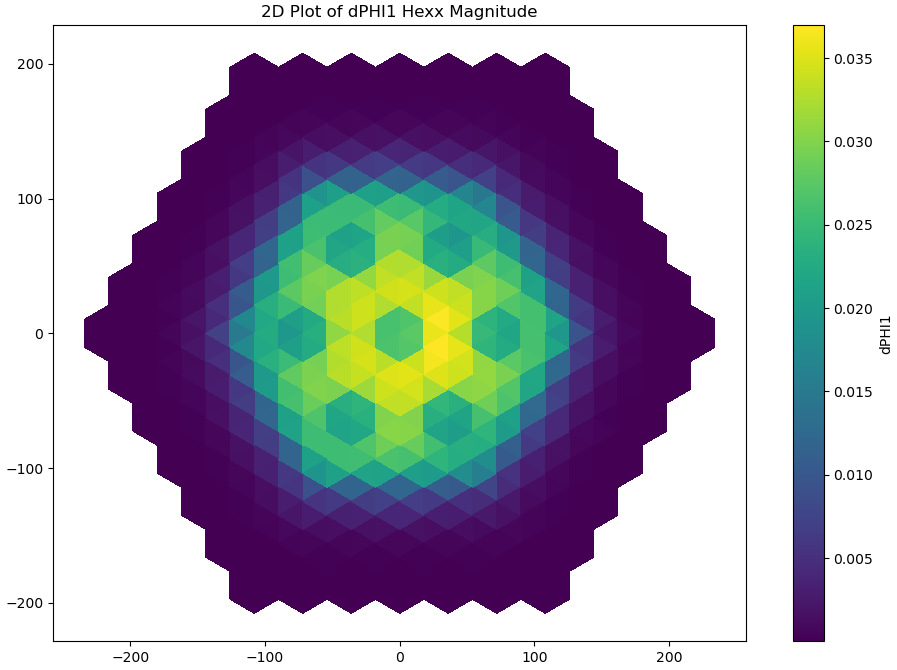
\includegraphics[width=\linewidth]{figures/OBJECTIVES3_TEST03_2DTriMG_HTTR2G_AVS_level1_NOISE_dPHI_magnitude_G1.png}
        \end{subfigure}
        \hfill
        \begin{subfigure}{.48\textwidth}
          \centering
          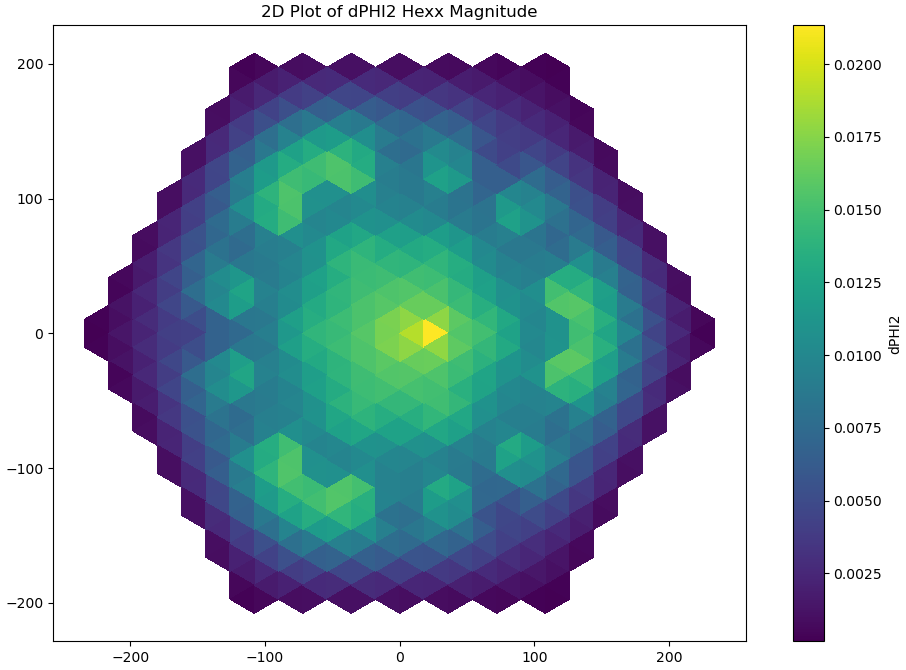
\includegraphics[width=\linewidth]{figures/OBJECTIVES3_TEST03_2DTriMG_HTTR2G_AVS_level1_NOISE_dPHI_magnitude_G2.png}
        \end{subfigure}
        \caption{Magnitude of the neutron noise for AVS in 2D HTTR}
        \label{fig:2DHTTR_noise_results_mag}
\end{figure}
\begin{figure}[H]
        \centering
        \begin{subfigure}{.48\textwidth}
          \centering
          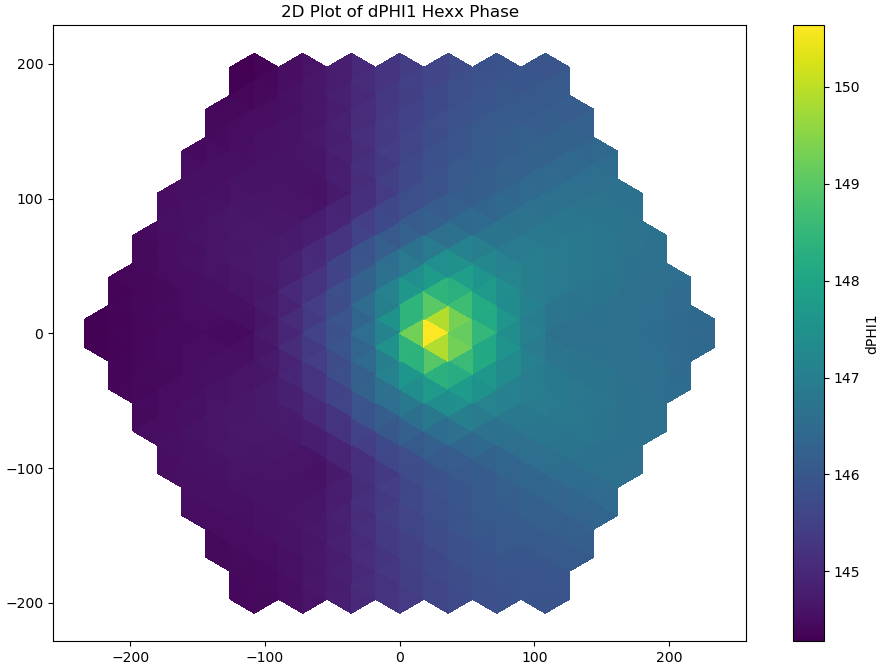
\includegraphics[width=\linewidth]{figures/OBJECTIVES3_TEST03_2DTriMG_HTTR2G_AVS_level1_NOISE_dPHI_phase_G1.png}
        \end{subfigure}
        \hfill
        \begin{subfigure}{.48\textwidth}
          \centering
          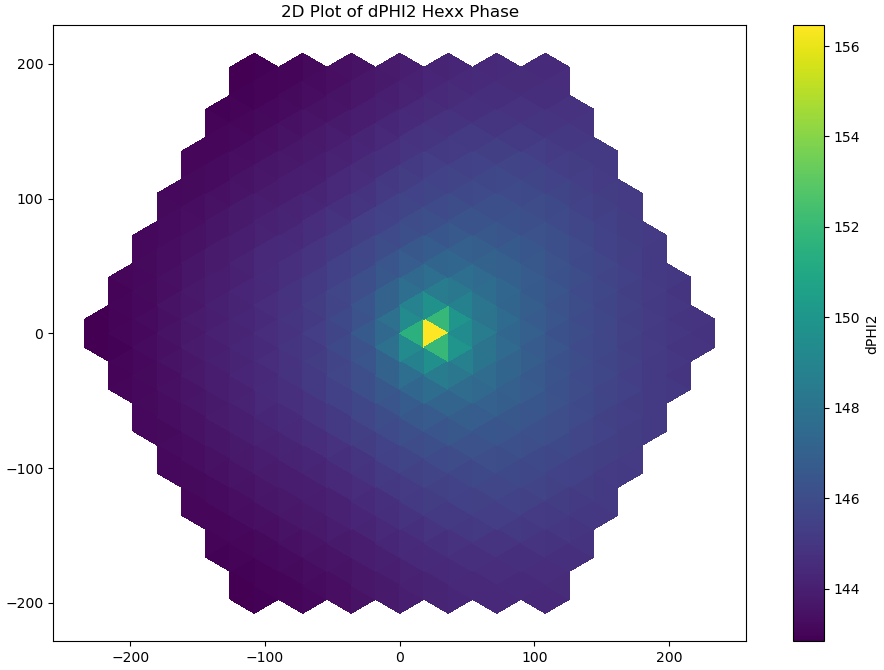
\includegraphics[width=\linewidth]{figures/OBJECTIVES3_TEST03_2DTriMG_HTTR2G_AVS_level1_NOISE_dPHI_phase_G2.png}
        \end{subfigure}
        \caption{Phase of the neutron noise for AVS in 2D HTTR}
        \label{fig:2DHTTR_noise_results_phase}
\end{figure}

Generally, the results indicate that the effect of neutron noise is more apparent in the thermal group. This is mainly due to the noise source located in the thermal spectrum only. We can also see in the phase delay plot (Figure \ref{fig:2DHTTR_noise_results_phase}) that the effect of neutron noise is more localized in the thermal group compared to the fast group. It should be noted that even though the neutron noise source is located at the thermal group only, the neutron noise in the fast group has a larger magnitude and is more dispersed compared to the thermal group. This is expected due to the larger mean free path of fast neutrons.

To further understand the driving force of neutron noise, we can split the neutron noise into its point kinetic component and its spatial component, as shown in Eq. \ref{eq:noise_component_time}. Figures \ref{fig:2DHTTRAVS_noise_component_results1} and \ref{fig:2DHTTRAVS_noise_component_results2} show the point kinetic component and spatial component of the neutron noise in fast and thermal group with AVS source, taken at the centerline of the core ($y=0$).
\begin{figure}[H]
        \centering
        \begin{subfigure}{.48\textwidth}
          \centering
          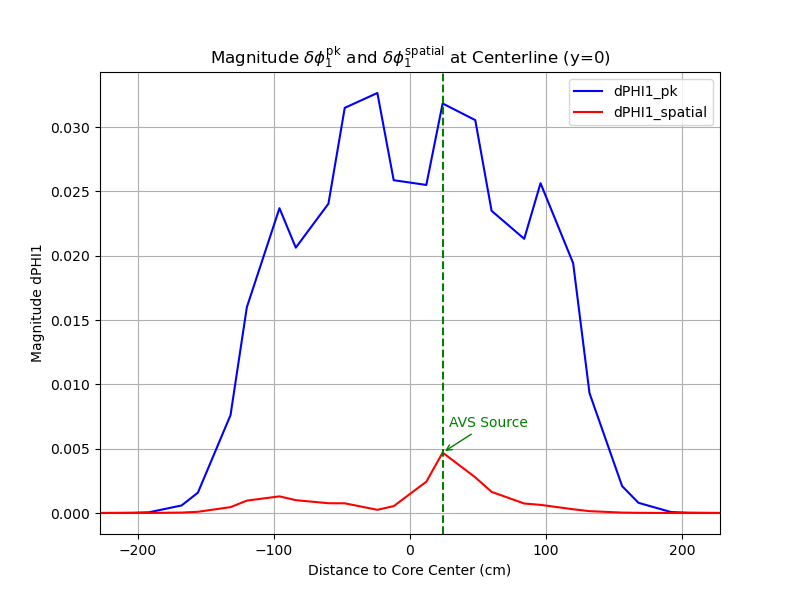
\includegraphics[width=\linewidth]{figures/Centerline_y0_OBJECTIVES3_TEST03_2DTriMG_HTTR2G_AVS_level1_dPHI_magnitude_G1.png}
        \end{subfigure}
        \hfill
        \begin{subfigure}{.48\textwidth}
          \centering
          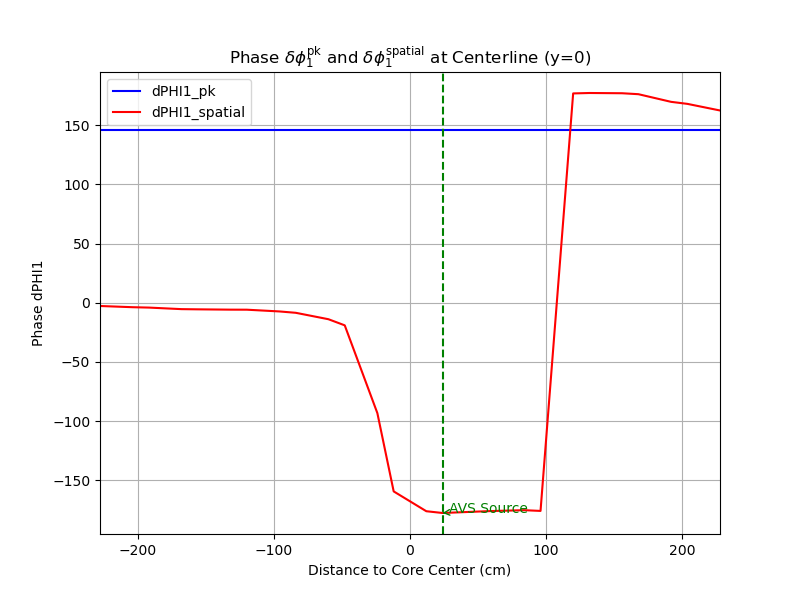
\includegraphics[width=\linewidth]{figures/Centerline_y0_OBJECTIVES3_TEST03_2DTriMG_HTTR2G_AVS_level1_dPHI_phase_G1.png}
        \end{subfigure}
        \caption{Magnitude (left) and phase (right) of the components of fast neutron noise for AVS in 2D HTTR, taken at centerline ($y=0$)}
        \label{fig:2DHTTRAVS_noise_component_results1}
\end{figure}
\begin{figure}[H]
        \centering
        \begin{subfigure}{.48\textwidth}
          \centering
          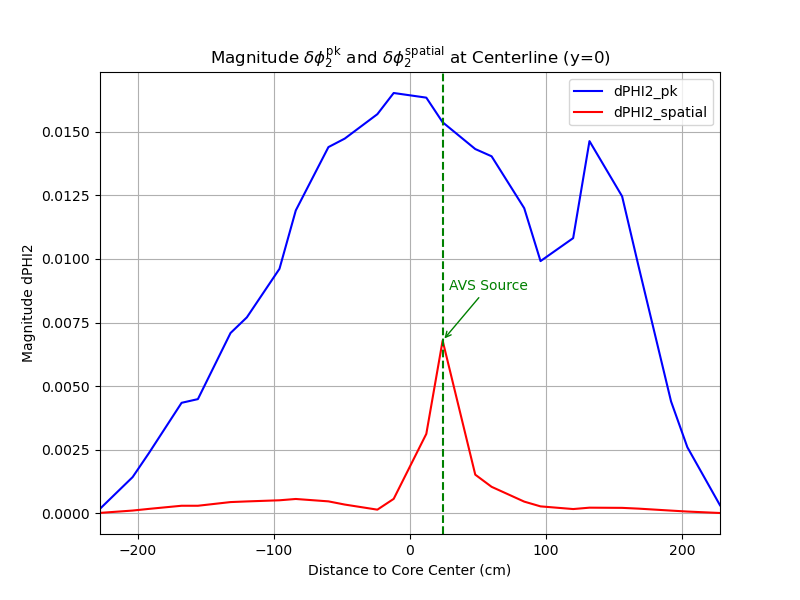
\includegraphics[width=\linewidth]{figures/Centerline_y0_OBJECTIVES3_TEST03_2DTriMG_HTTR2G_AVS_level1_dPHI_magnitude_G2.png}
        \end{subfigure}
        \hfill
        \begin{subfigure}{.48\textwidth}
          \centering
          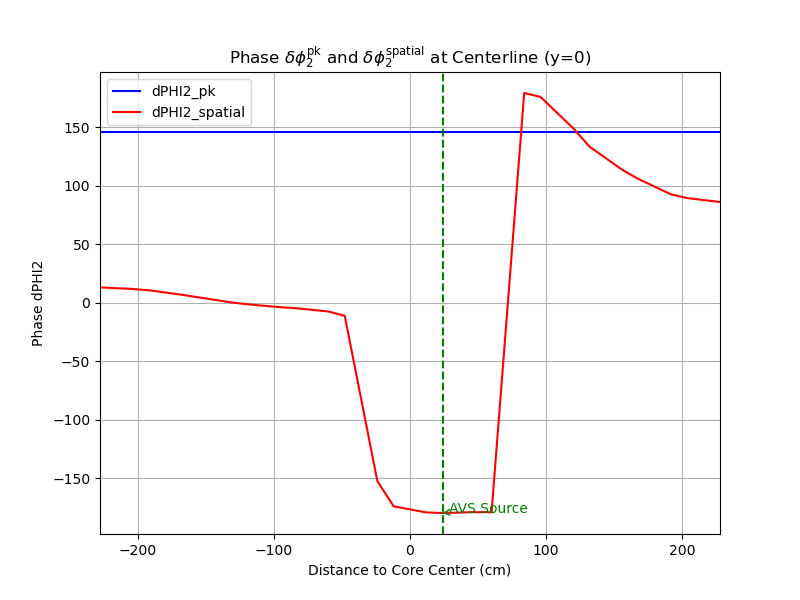
\includegraphics[width=\linewidth]{figures/Centerline_y0_OBJECTIVES3_TEST03_2DTriMG_HTTR2G_AVS_level1_dPHI_phase_G2.png}
        \end{subfigure}
        \caption{Magnitude (left) and phase (right) of the components of thermal neutron noise for AVS in 2D HTTR, taken at centerline ($y=0$)}
        \label{fig:2DHTTRAVS_noise_component_results2}
\end{figure}
Comparing Figure \ref{fig:2DHTTRAVS_noise_component_results1} and Figure \ref{fig:2DHTTRAVS_noise_component_results2}, we can see that in the fast group, the magnitude of the point kinetic component is has higher magnitude compared to the spatial component. This makes the magnitude of the neutron noise in the fast group more dispersed, following the point kinetic component. In the thermal group, the point kinetic component is also higher compared to the spatial component, but not at the same ratio as the fast group. This makes the contribution of the spatial component more apparent in the thermal group. The variation of the phase delay is mainly driven by the spatial components. This means that the phase of the spatial component drives the out-of-phase behavior of the neutron noise in the system. It is expected that the point kinetic component will have no effect on the phase delays since it is a factor of the forward flux. Overall, we can see that the point kinetic component is more dominant in 2D HTTR, which means that the neutron noise is driven by the reactivity effect of the perturbation.

\subsection{2D HTTR with Fuel Assembly Vibration Source}

For the simulation of the fuel assembly vibration, the neutron noise source is modeled using the $\varepsilon/d$ method. This means perturbation is a time-dependent sinusoidal function with amplitude $\varepsilon$ and frequency $\omega_0$. In this case, the frequency of vibration ($\omega_0$) is defined as 1 Hz, and the amplitude of vibration ($\varepsilon$) is 0.5 cm. Using this definition, the neutron noise source model is written as follows:
\begin{equation}
    \delta \Sigma_{a,g} (\textbf{r}_b,\omega) = \left\{
\begin{array}{ll}
      -i \pi \varepsilon \Delta  \Sigma_{a,g} \delta (\omega - \omega_0) & \textbf{r}_b-\varepsilon\leq y \leq \textbf{r}_b + \varepsilon \\
      0 & \text{otherwise}\\
\end{array} 
\right. 
\end{equation}
This means that all the interfaces of the assembly become the source of neutron noise. This differs from rectangular geometry cases, where the vibration can be defined in one axis and the other axis remains constant. The vibration is located at assembly number 65, as shown in Figure \ref{fig:HTTR2DFAV}.
\begin{figure}[H]
        \centering
        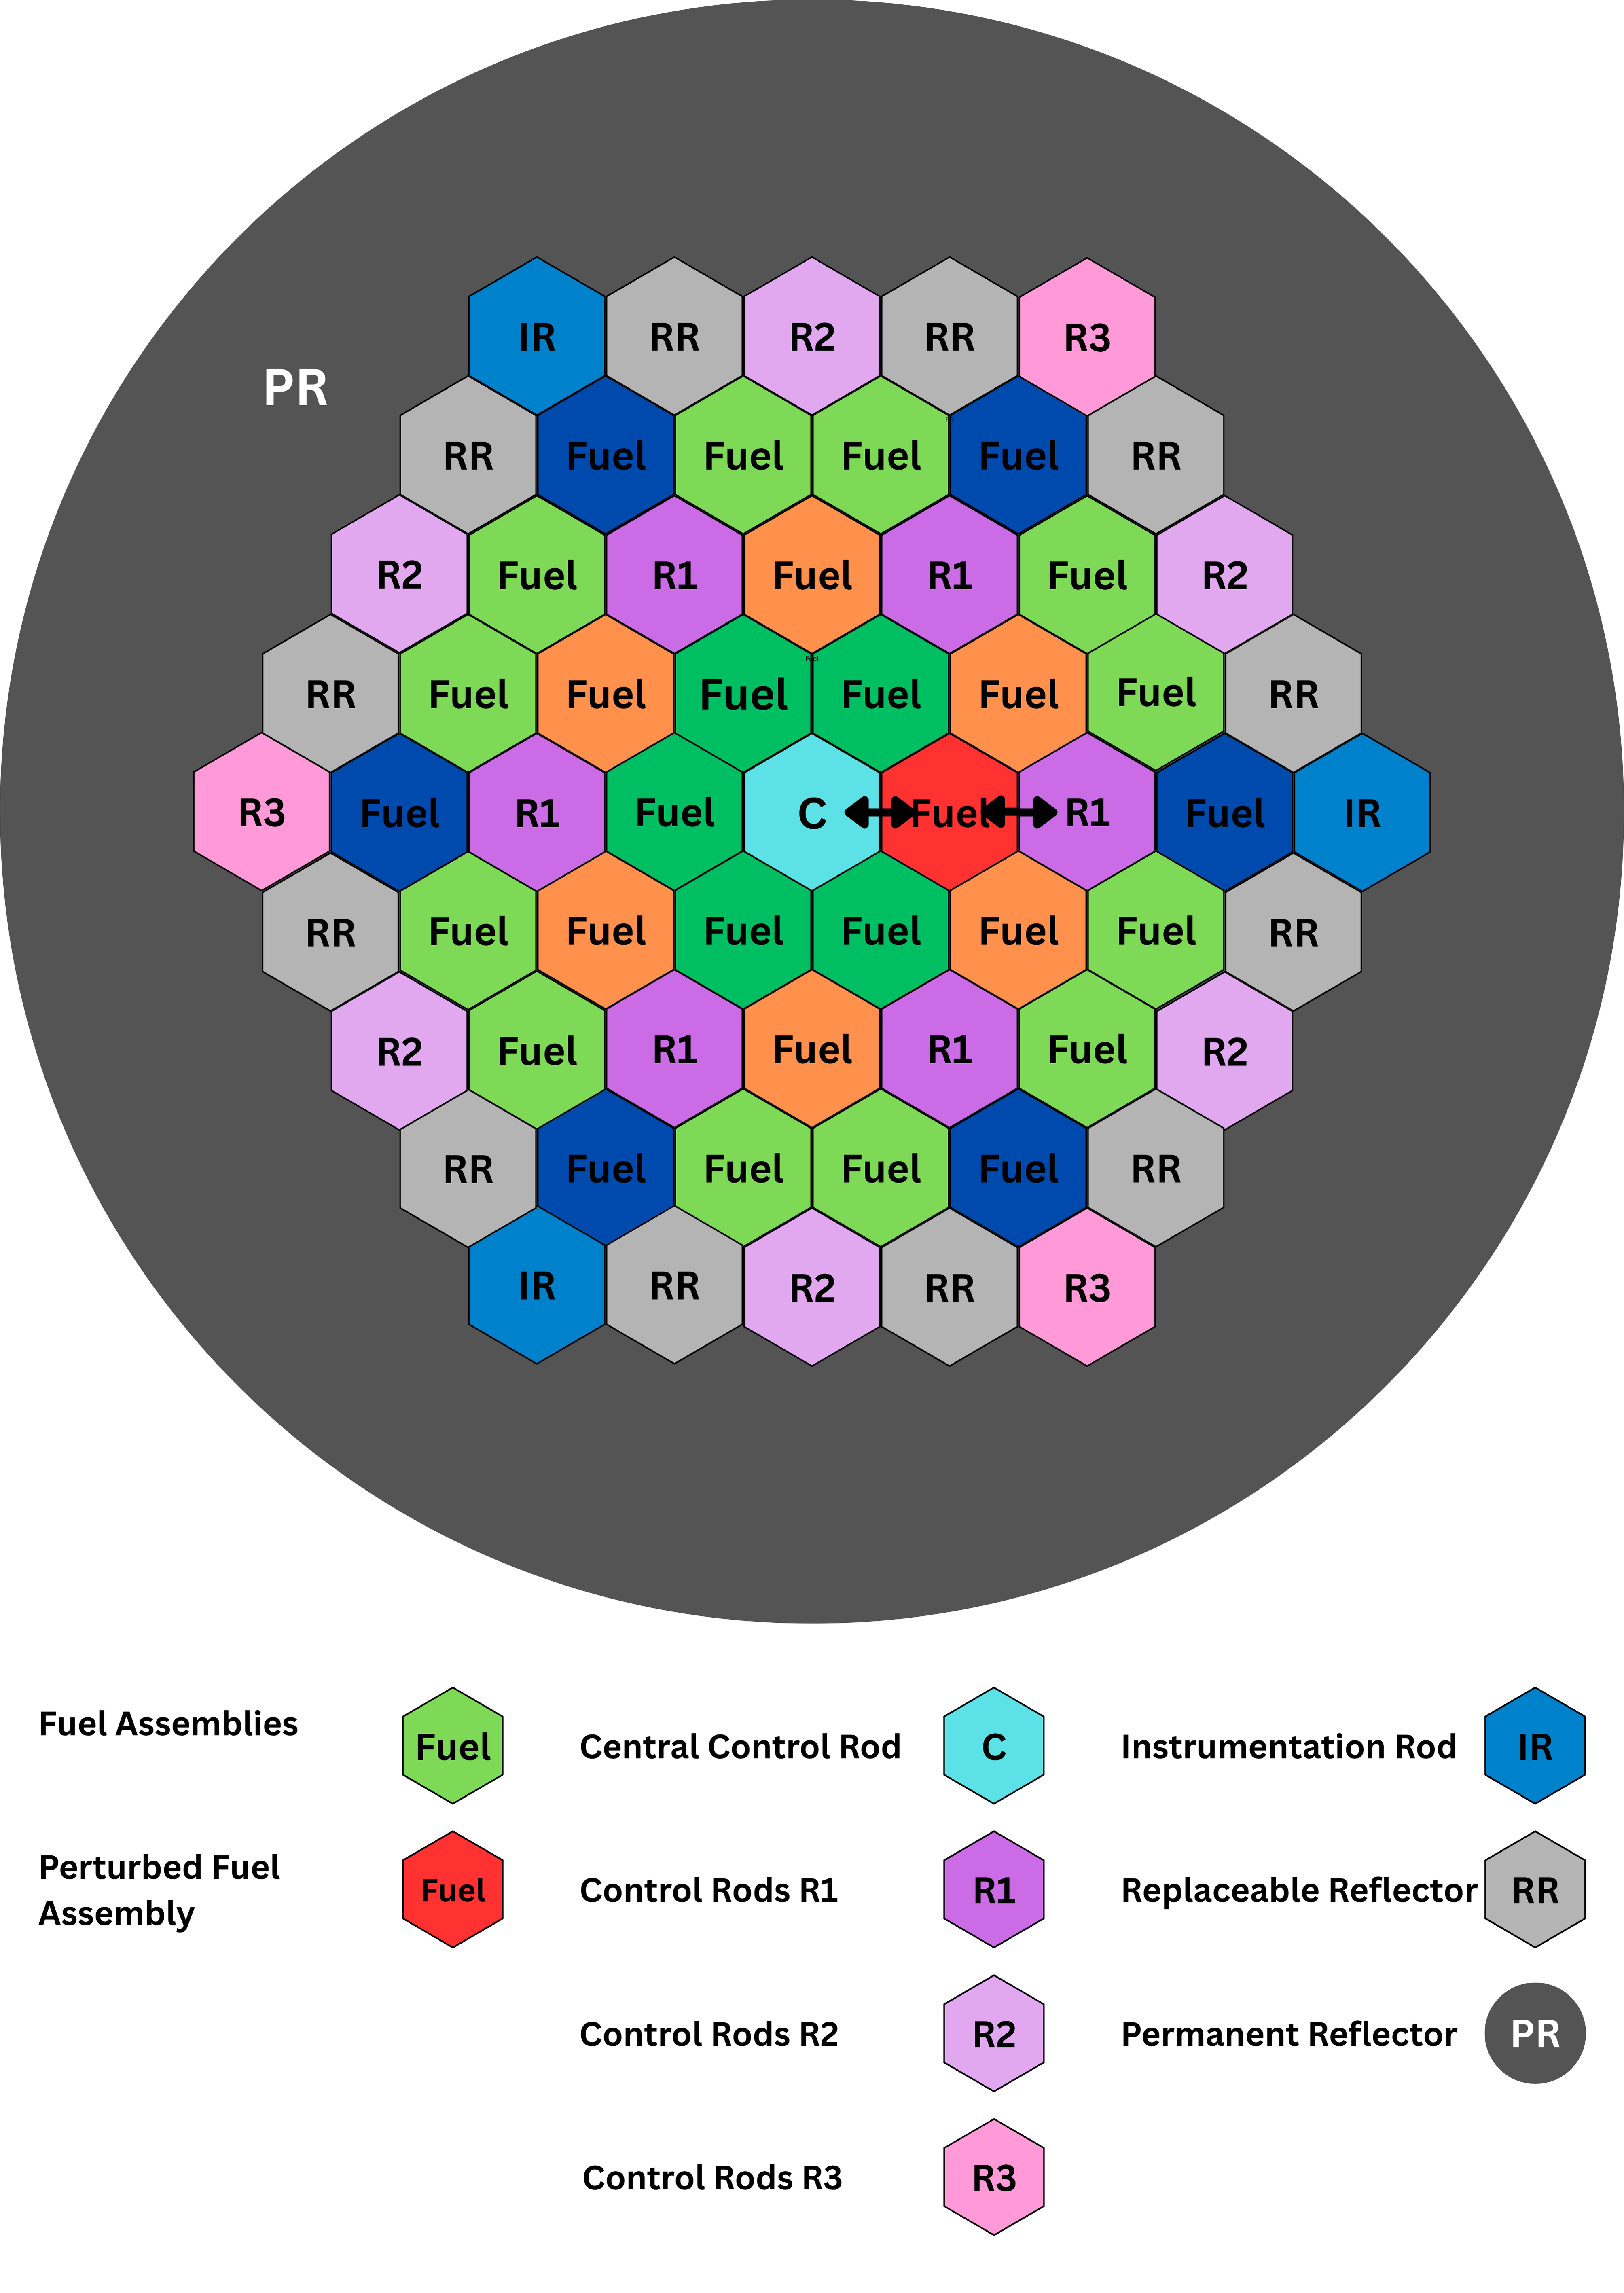
\includegraphics[width=0.45\textwidth]{figures/HTTR2DFAV.png}
        \caption{Location of the fuel assembly vibration for 2D HTTR}
        \label{fig:HTTR2DFAV}
\end{figure}
The results of the simulations are as follows:
\begin{figure}[H]
        \centering
        \begin{subfigure}{.48\textwidth}
          \centering
          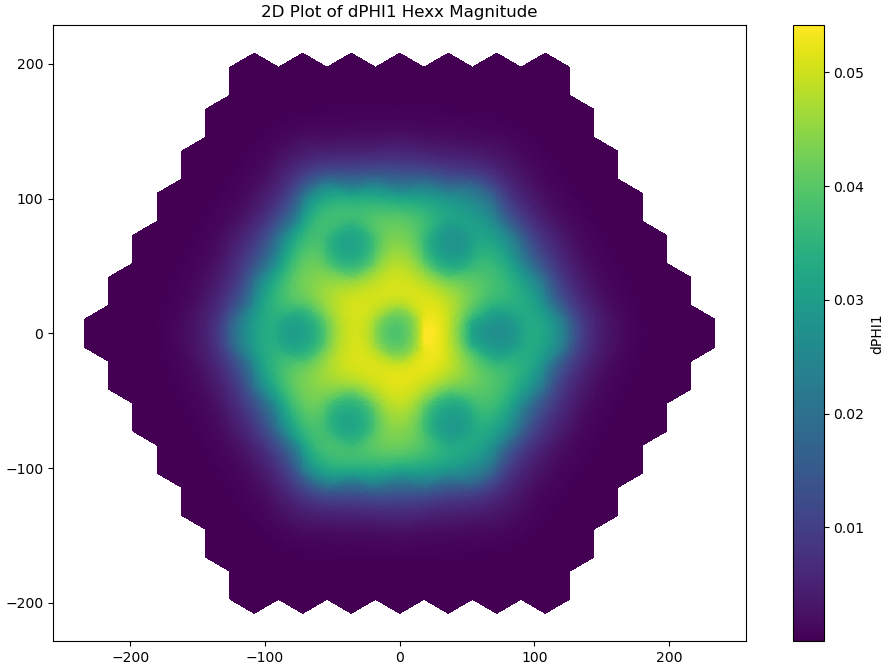
\includegraphics[width=\linewidth]{figures/OBJECTIVES3_TEST04_2DTriMG_HTTR2G_FAV_level5_NOISE_dPHI_magnitude_G1.png}
        \end{subfigure}
        \hfill
        \begin{subfigure}{.48\textwidth}
          \centering
          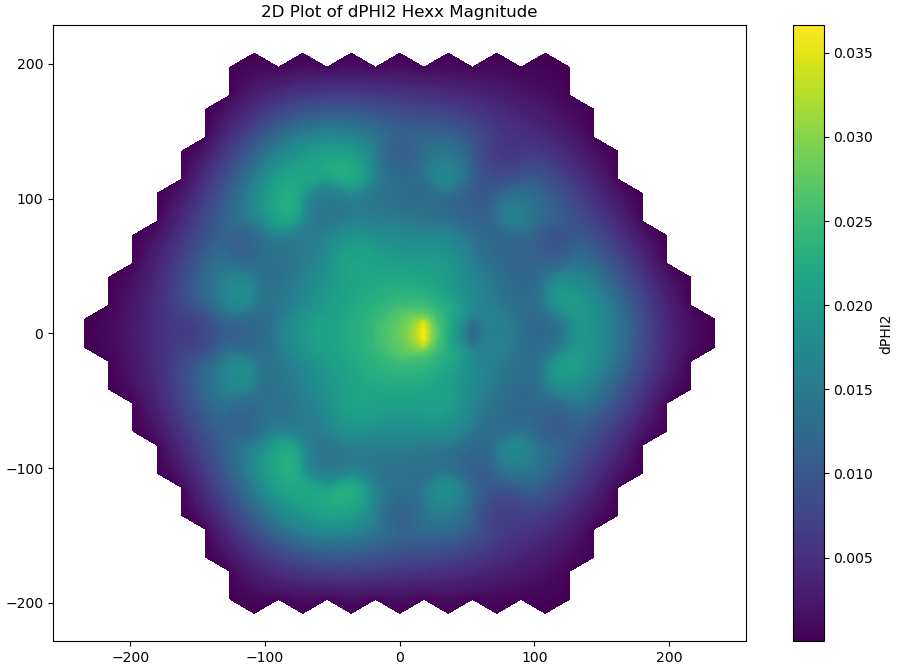
\includegraphics[width=\linewidth]{figures/OBJECTIVES3_TEST04_2DTriMG_HTTR2G_FAV_level5_NOISE_dPHI_magnitude_G2.png}
        \end{subfigure}
        \caption{Magnitude of the neutron noise for FAV in 2D HTTR}
        \label{fig:2DHTTR_noise_FAV_results_mag}
\end{figure}
\begin{figure}[H]
        \centering
        \begin{subfigure}{.48\textwidth}
          \centering
          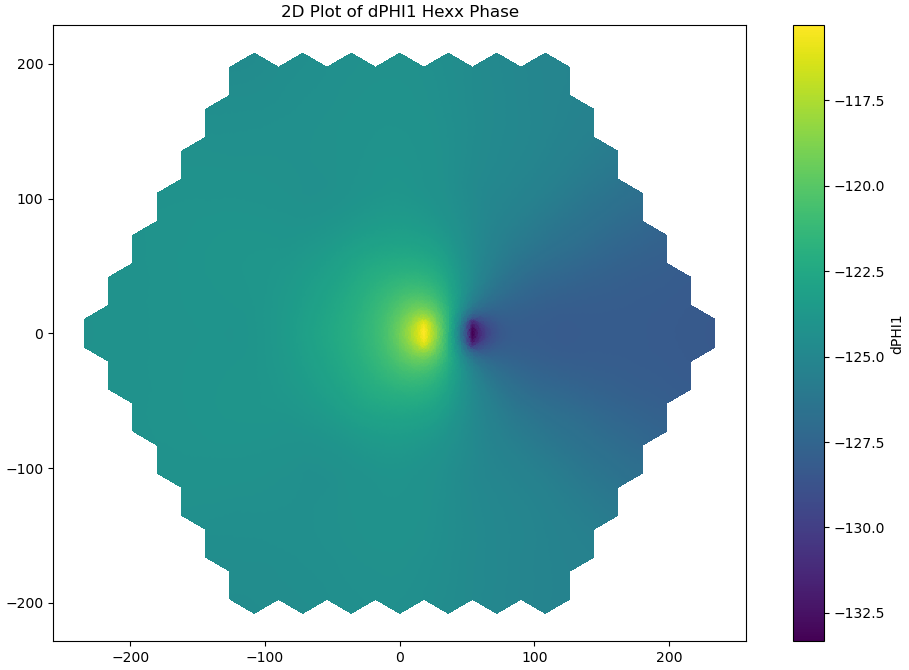
\includegraphics[width=\linewidth]{figures/OBJECTIVES3_TEST04_2DTriMG_HTTR2G_FAV_level5_NOISE_dPHI_phase_G1.png}
        \end{subfigure}
        \hfill
        \begin{subfigure}{.48\textwidth}
          \centering
          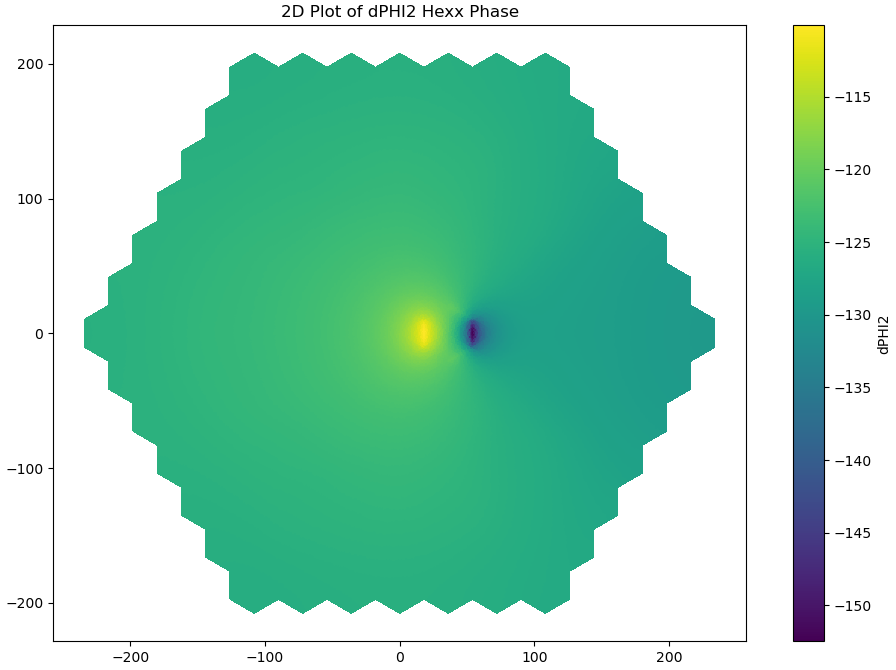
\includegraphics[width=\linewidth]{figures/OBJECTIVES3_TEST04_2DTriMG_HTTR2G_FAV_level5_NOISE_dPHI_phase_G2.png}
        \end{subfigure}
        \caption{Phase of the neutron noise for FAV in 2D HTTR}
        \label{fig:2DHTTR_noise_FAV_results_phase}
\end{figure}

As seen in Figure \ref{fig:2DHTTR_noise_FAV_results_mag} and Figure \ref{fig:2DHTTR_noise_FAV_results_phase}, the neutron noise is more apparent in the thermal group and more dispersed in the fast group. This is a similar phenomenon compared to the AVS source in 2D HTTR. For the fuel assembly vibration case, it is expected that there will be some opposing effect in the magnitude and phase delay results due to the out-of-phase neutron noise source model. This is clearly evident in the simulation. Since the vibrating assembly is a fuel assembly, the opposing effect is not so apparent in the interfaces where the neighboring assembly is also a fuel assembly. This is expected since the difference between the macroscopic cross-sections  ($\Delta \Sigma_{a,g}$) is smaller at these interfaces. However, the opposing effect becomes more evident at the interfaces where the neighboring assembly is a reflector assembly. 

To further understand the driving force of neutron noise, we can split the neutron noise into its point kinetic component and its spatial component. Figures \ref{fig:2DHTTRFAV_noise_component_results1} and \ref{fig:2DHTTRFAV_noise_component_results2} show the point kinetic component and spatial component of the neutron noise in fast and thermal group with FAV source, taken at the centerline of the core ($y=0$).

\begin{figure}[H]
        \centering
        \begin{subfigure}{.48\textwidth}
          \centering
          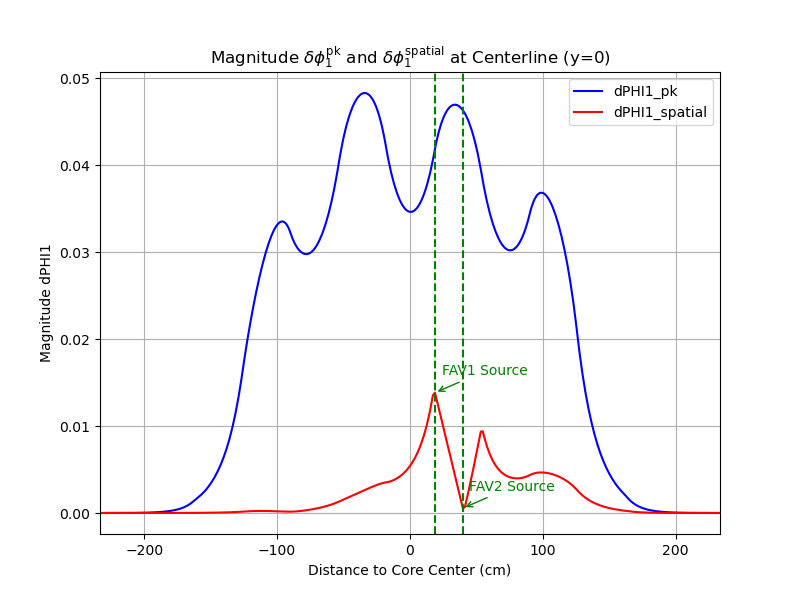
\includegraphics[width=\linewidth]{figures/Centerline_y0_OBJECTIVES3_TEST04_2DTriMG_HTTR2G_FAV_level5_dPHI_magnitude_G1.png}
        \end{subfigure}
        \hfill
        \begin{subfigure}{.48\textwidth}
          \centering
          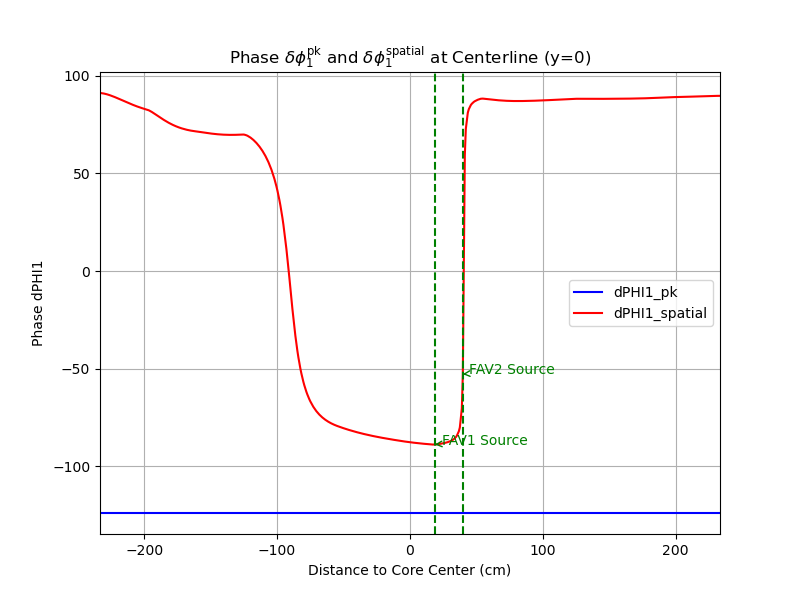
\includegraphics[width=\linewidth]{figures/Centerline_y0_OBJECTIVES3_TEST04_2DTriMG_HTTR2G_FAV_level5_dPHI_phase_G1.png}
        \end{subfigure}
        \caption{Magnitude (left) and phase (right) of the components of fast neutron noise for FAV in 2D HTTR, taken at centerline ($y=0$)}
        \label{fig:2DHTTRFAV_noise_component_results1}
\end{figure}
\begin{figure}[H]
        \centering
        \begin{subfigure}{.48\textwidth}
          \centering
          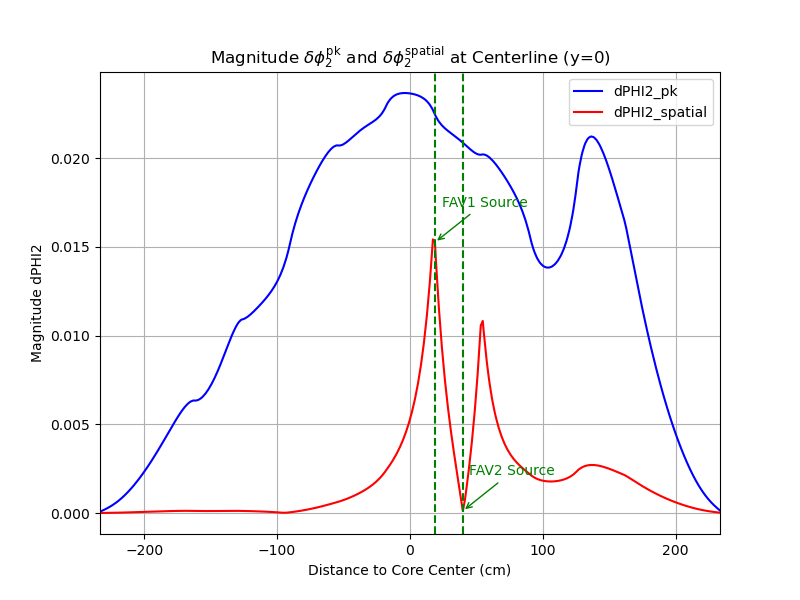
\includegraphics[width=\linewidth]{figures/Centerline_y0_OBJECTIVES3_TEST04_2DTriMG_HTTR2G_FAV_level5_dPHI_magnitude_G2.png}
        \end{subfigure}
        \hfill
        \begin{subfigure}{.48\textwidth}
          \centering
          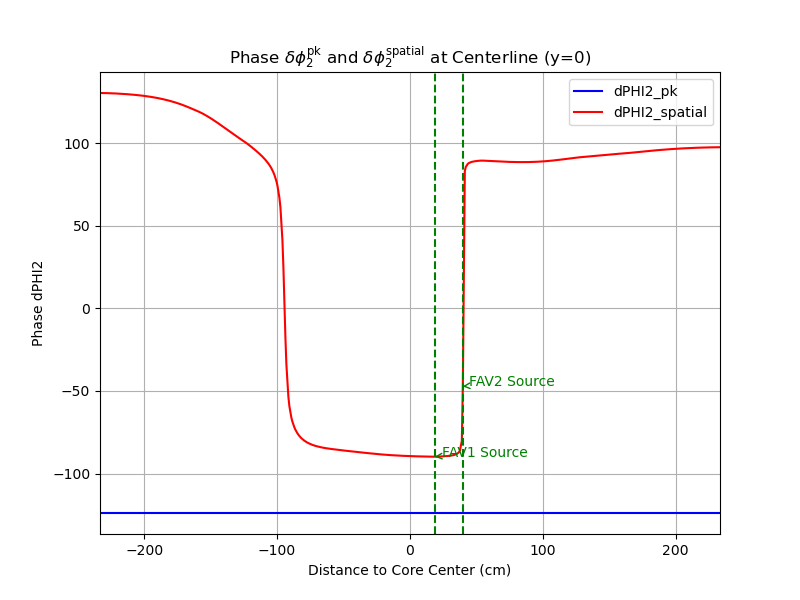
\includegraphics[width=\linewidth]{figures/Centerline_y0_OBJECTIVES3_TEST04_2DTriMG_HTTR2G_FAV_level5_dPHI_phase_G2.png}
        \end{subfigure}
        \caption{Magnitude (left) and phase (right) of the components of thermal neutron noise for FAV in 2D HTTR, taken at centerline ($y=0$)}
        \label{fig:2DHTTRFAV_noise_component_results2}
\end{figure}
Comparing Figure \ref{fig:2DHTTRFAV_noise_component_results1}, and Figure \ref{fig:2DHTTRFAV_noise_component_results2}, we can see that the behavior is similar to the AVS source, where the point kinetic component is more apparent in the magnitude of neutron noise. The point kinetic component in the fast group is more dominant compared to the thermal group, which makes the magnitude of the neutron noise in the fast group more dispersed. The opposing effect of the neutron noise source is reflected in the magnitude of the neutron noise source. The spatial component influences the phase delays similarly to the AVS source. The out-of-phase behavior can be clearly seen in the phases of the neutron noise. In general, we can see that the point kinetic component has a more significant impact on the magnitude of neutron noise, while the spatial component affects the phase of the neutron noise. 

\subsection{3D HTTR with Absorber of Variable Strength Source}

For this simulation, the neutron noise source is defined as perturbation of the thermal absorption cross-section in the fuel assembly. Formally, the perturbation can be written as follows:
\begin{equation}
    \delta \Sigma_{a,2}(\textbf{r}, \omega) = \gamma(\omega) \delta(\textbf{r} - \textbf{r}_0)
\end{equation}
Where $\gamma(\omega)$ is defined as 5\% of the thermal absorption cross-section at $r_0$ and $r_0$ is defined as one triangle mesh in assembly number 65 at mid-elevation (mid-elevation of fuel zone 1, indicated as red triangle), which is shown in Figure \ref{fig:HTTR3DAVS}.
\begin{figure}[H]
        \centering
        \begin{subfigure}{.48\textwidth}
          \centering
          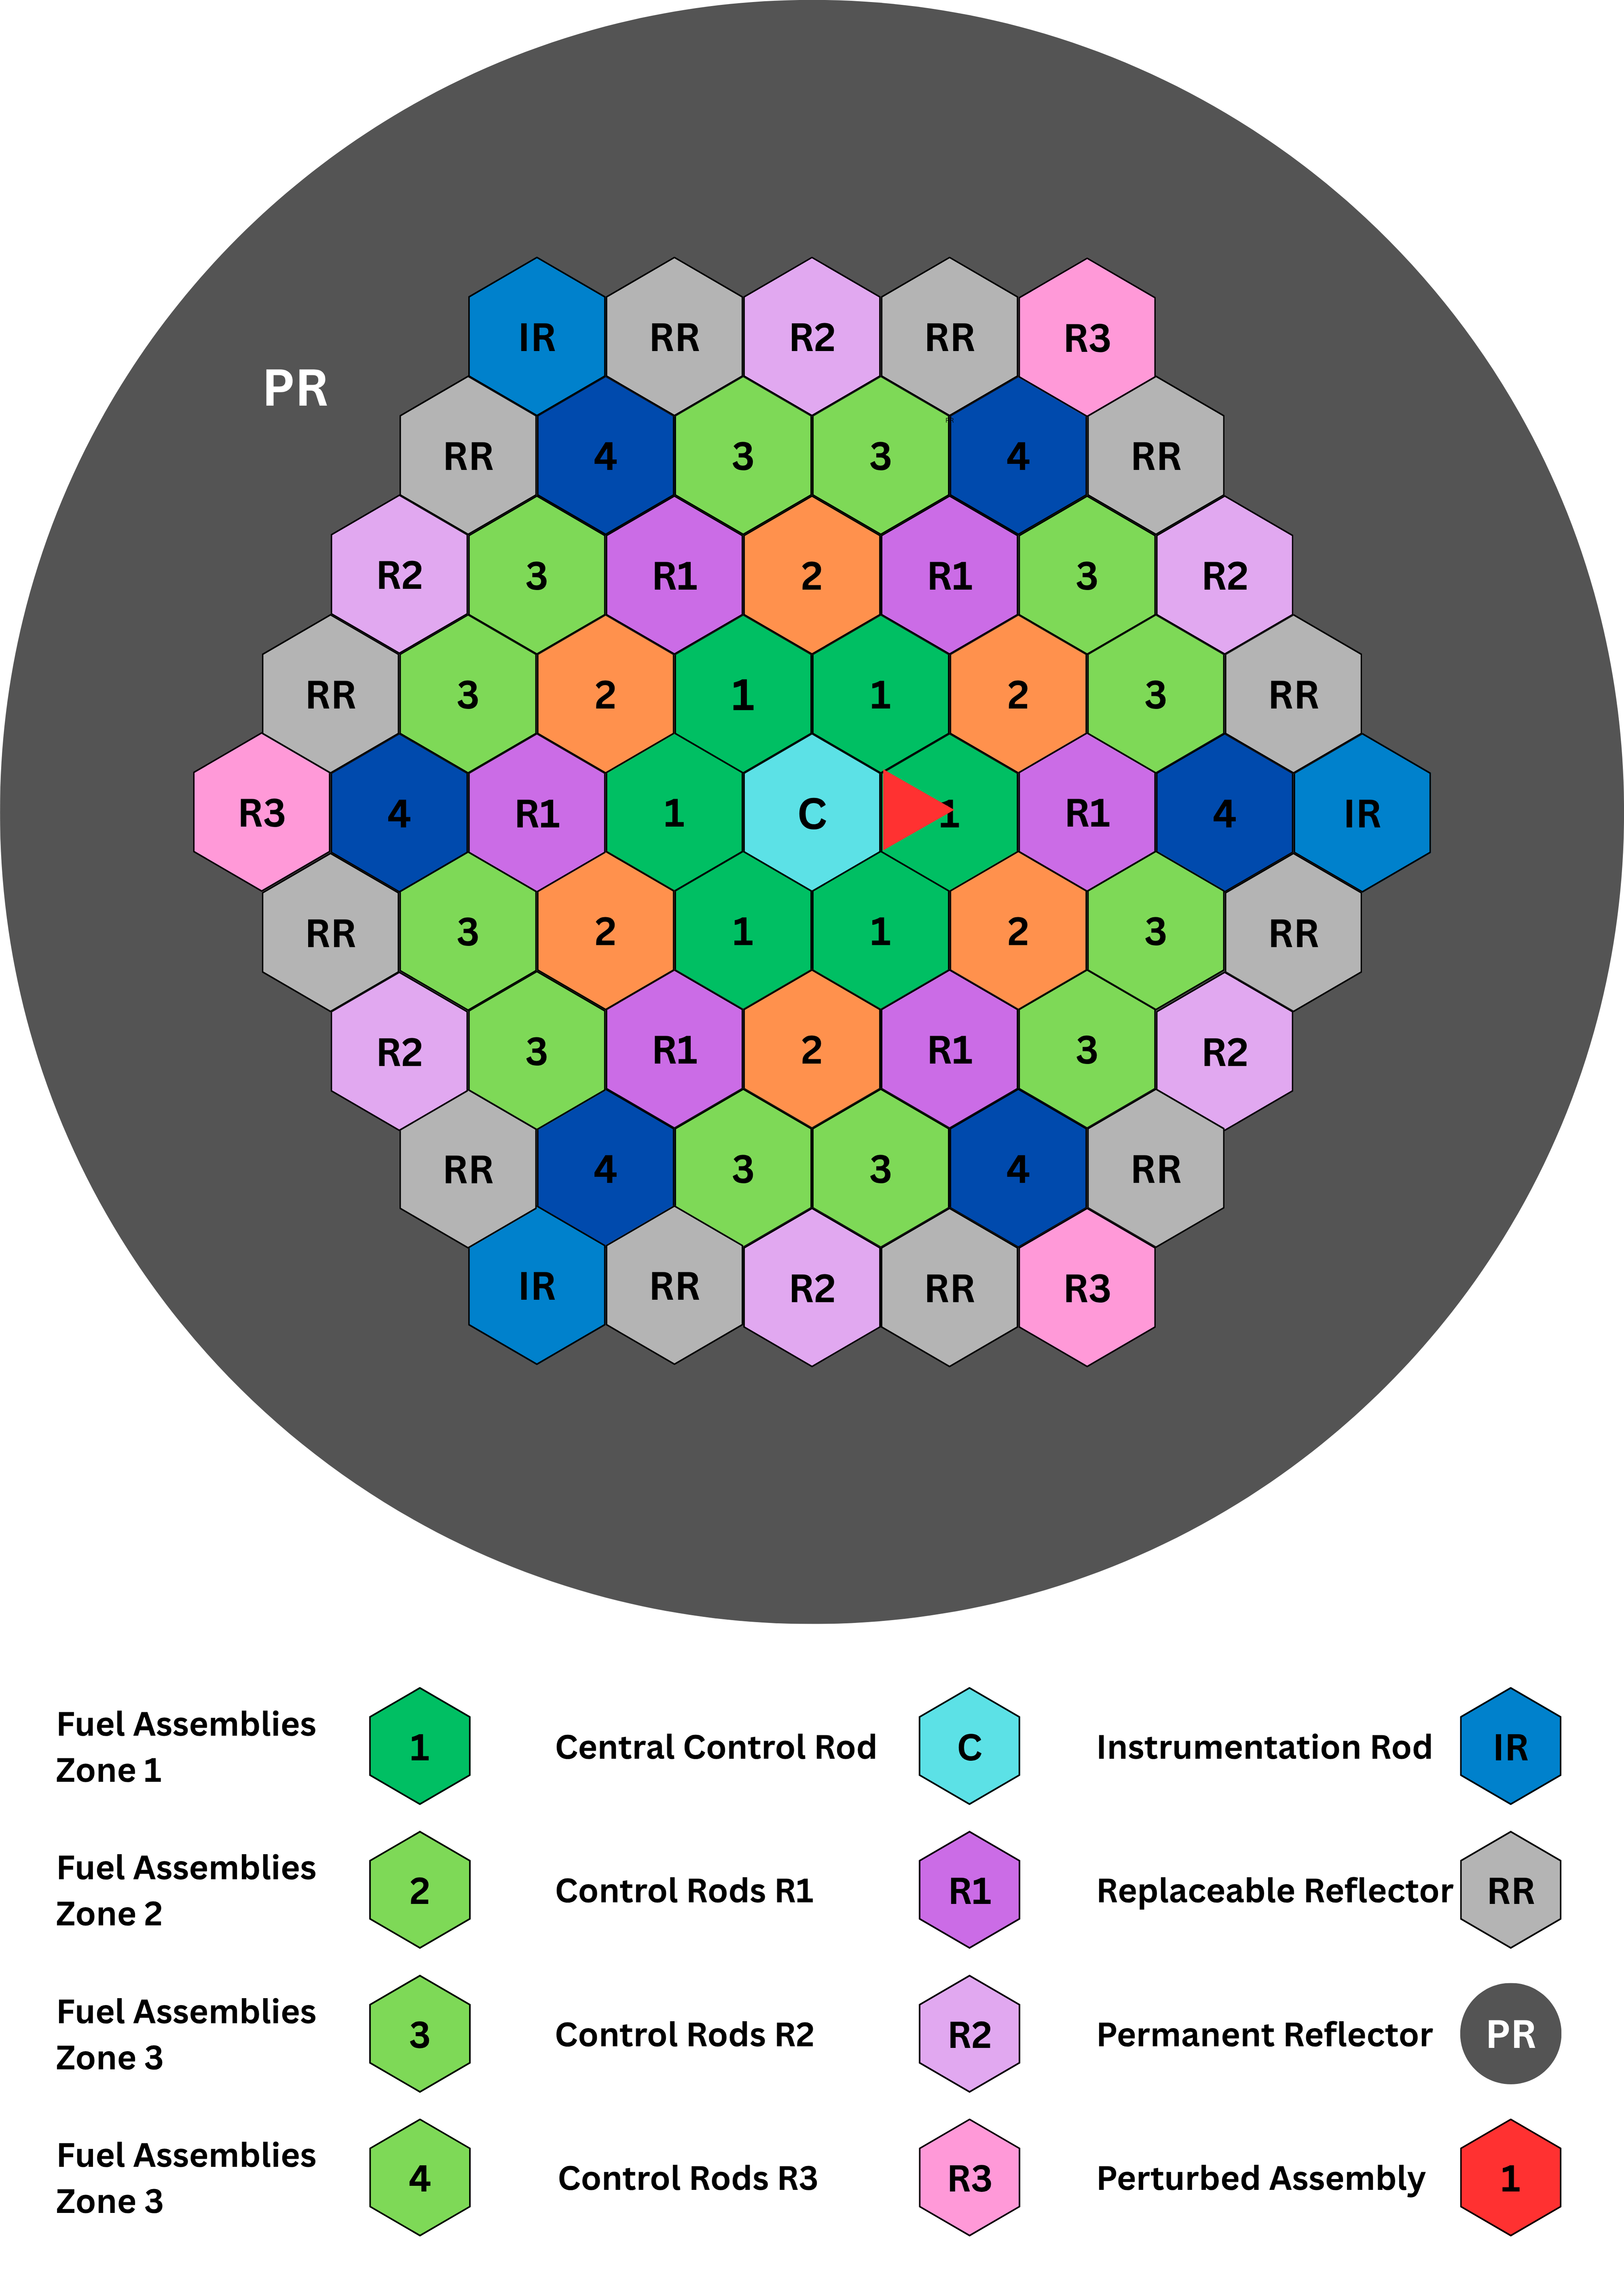
\includegraphics[width=\linewidth]{figures/HTTR3DAVS1.png}
        \end{subfigure}
        \hfill
        \begin{subfigure}{.48\textwidth}
          \centering
          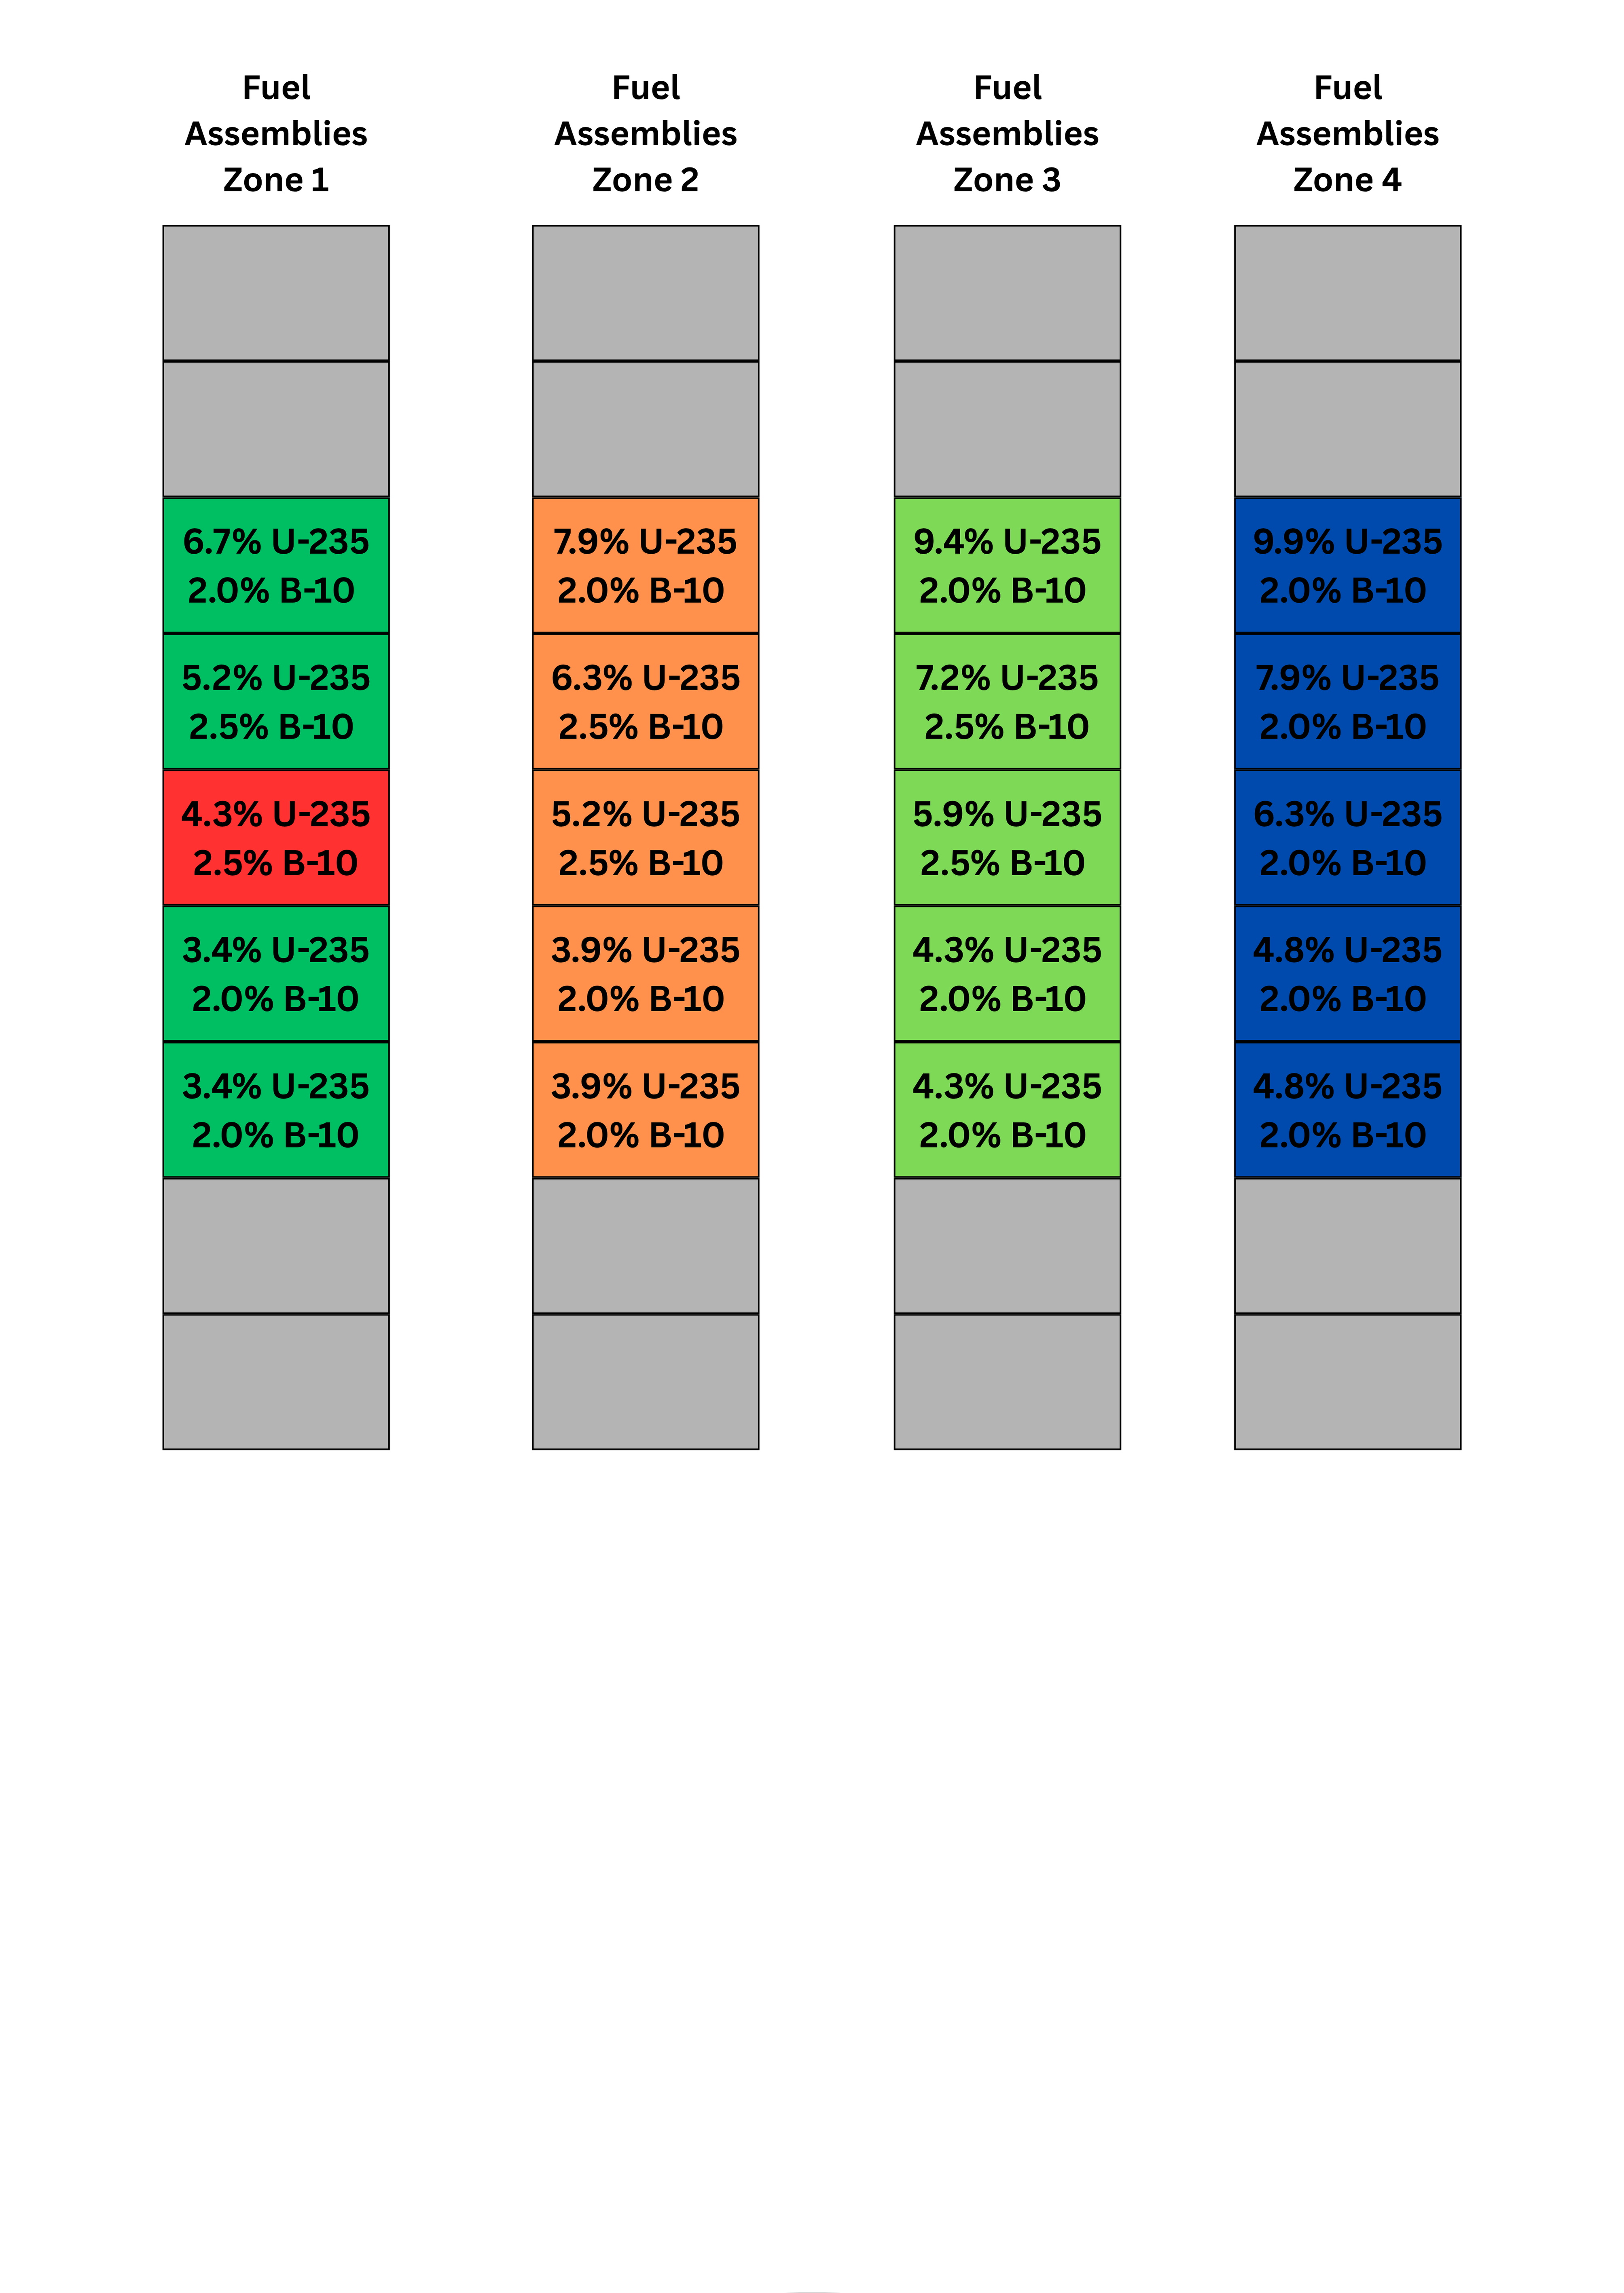
\includegraphics[width=\linewidth]{figures/HTTR3DAVS2.png}
        \end{subfigure}
        \caption{Location of the absorber of variable strength for 3D HTTR}
        \label{fig:HTTR3DAVS}
\end{figure}

The results of the simulations are as follows:
\begin{figure}[H]
        \centering
        \begin{subfigure}{.48\textwidth}
          \centering
          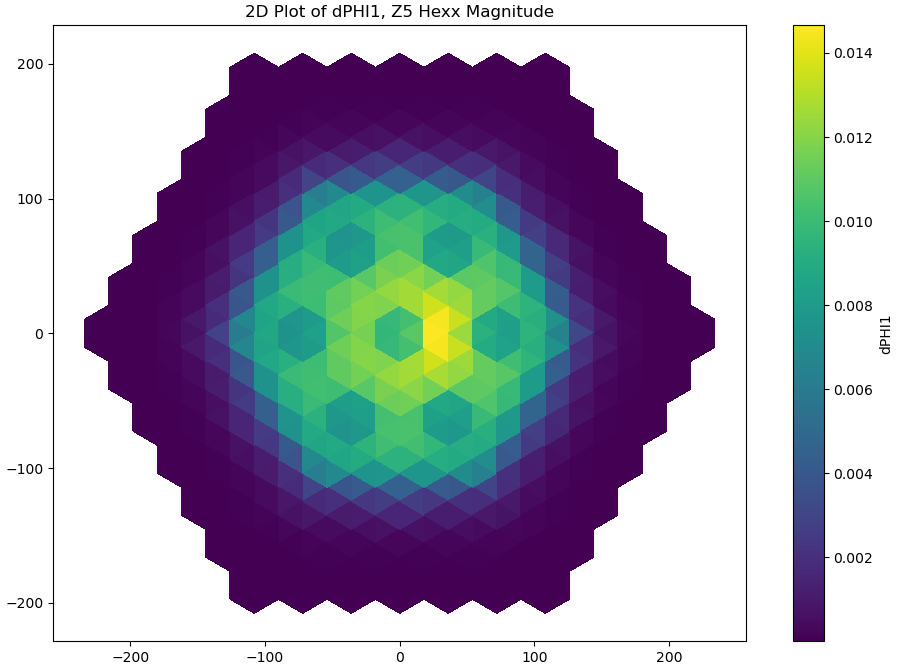
\includegraphics[width=\linewidth]{figures/OBJECTIVES3_TEST07_3DTriMG_HTTR_AVS_level1_NOISE_dPHI_magnitude_G1_Z5.png}
        \end{subfigure}
        \hfill
        \begin{subfigure}{.48\textwidth}
          \centering
          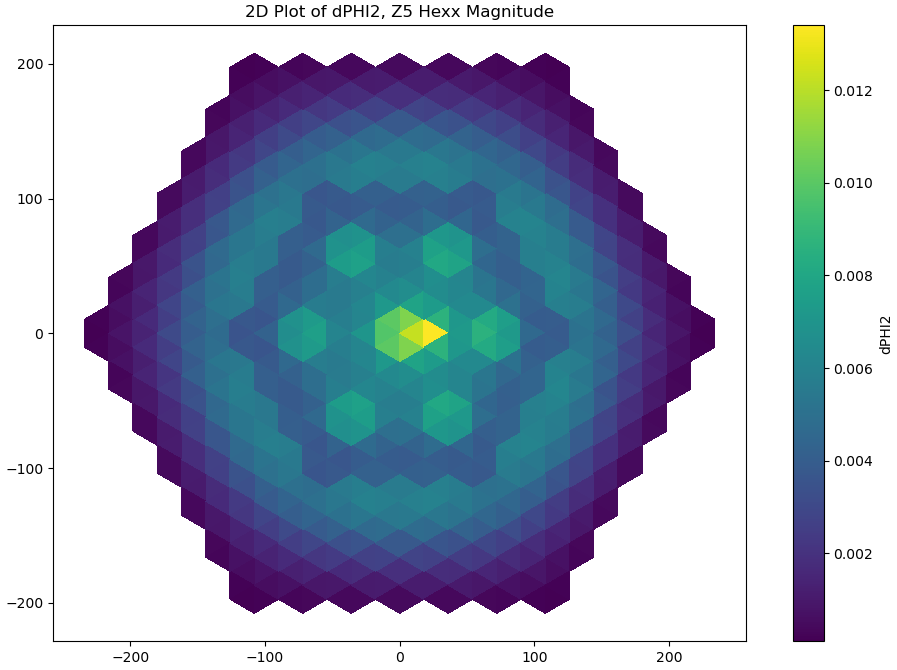
\includegraphics[width=\linewidth]{figures/OBJECTIVES3_TEST07_3DTriMG_HTTR_AVS_level1_NOISE_dPHI_magnitude_G2_Z5.png}
        \end{subfigure}
        \caption{Magnitude of the neutron noise for AVS in 3D HTTR at midplane ($Z = 5$)}
        \label{fig:3DHTTR_noise_AVS_results_mag}
\end{figure}
\begin{figure}[H]
        \centering
        \begin{subfigure}{.48\textwidth}
          \centering
          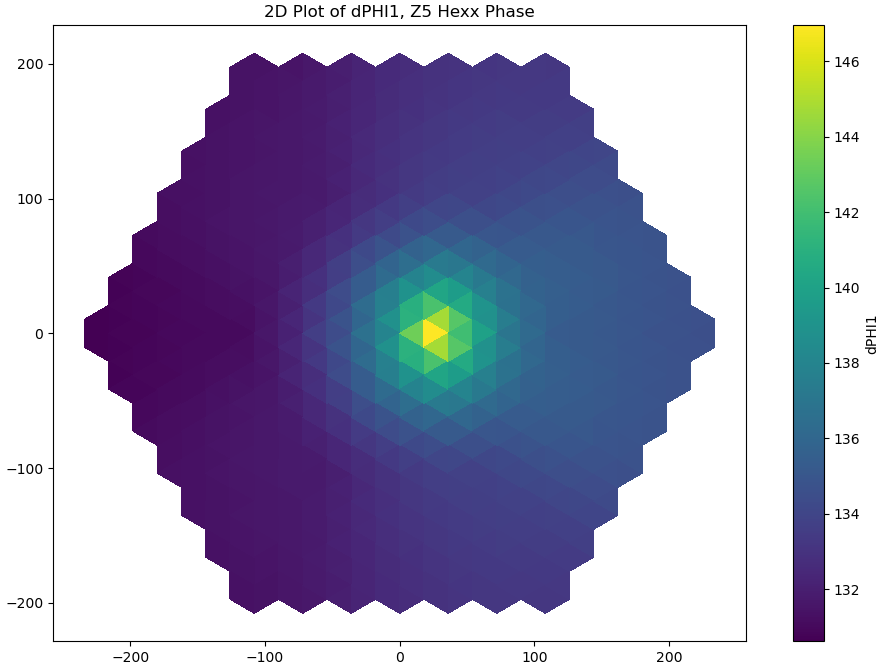
\includegraphics[width=\linewidth]{figures/OBJECTIVES3_TEST07_3DTriMG_HTTR_AVS_level1_NOISE_dPHI_phase_G1_Z5.png}
        \end{subfigure}
        \hfill
        \begin{subfigure}{.48\textwidth}
          \centering
          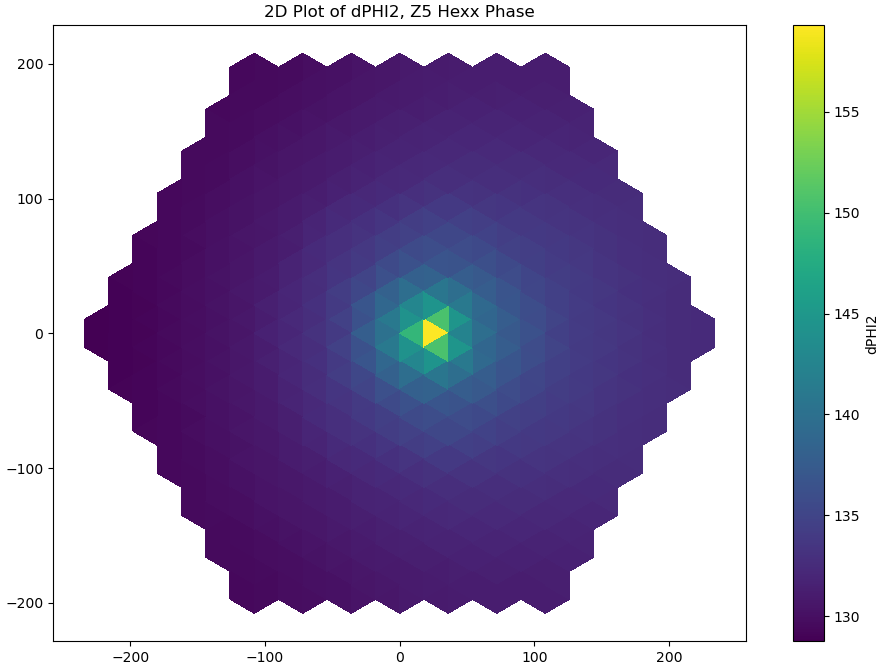
\includegraphics[width=\linewidth]{figures/OBJECTIVES3_TEST07_3DTriMG_HTTR_AVS_level1_NOISE_dPHI_phase_G2_Z5.png}
        \end{subfigure}
        \caption{Phase of the neutron noise for AVS in 3D HTTR at midplane ($Z = 5$)}
        \label{fig:3DHTTR_noise_AVS_results_phase}
\end{figure}

As shown in Figures \ref{fig:3DHTTR_noise_AVS_results_mag} and \ref{fig:3DHTTR_noise_AVS_results_phase}, the effect of neutron noise is more pronounced in the thermal group. This is mainly due to the noise source located in the thermal spectrum only. We can also see in the phase delay plot (Figure \ref{fig:3DHTTR_noise_AVS_results_phase}) that the effect of neutron noise is more localized in the thermal group compared to the fast group. This behavior is generally similar to the 2D HTTR case.

To further understand the driving force of neutron noise, we can split the neutron noise into its point kinetic component and its spatial component. Figures \ref{fig:3DHTTRAVS_noise_component_results1} and \ref{fig:3DHTTRAVS_noise_component_results2} show the point kinetic component and spatial component of the neutron noise in fast and thermal group with AVS source, taken at the centerline of the core ($y=0$) and midplane ($Z = 5$).

\begin{figure}[H]
        \centering
        \begin{subfigure}{.48\textwidth}
          \centering
          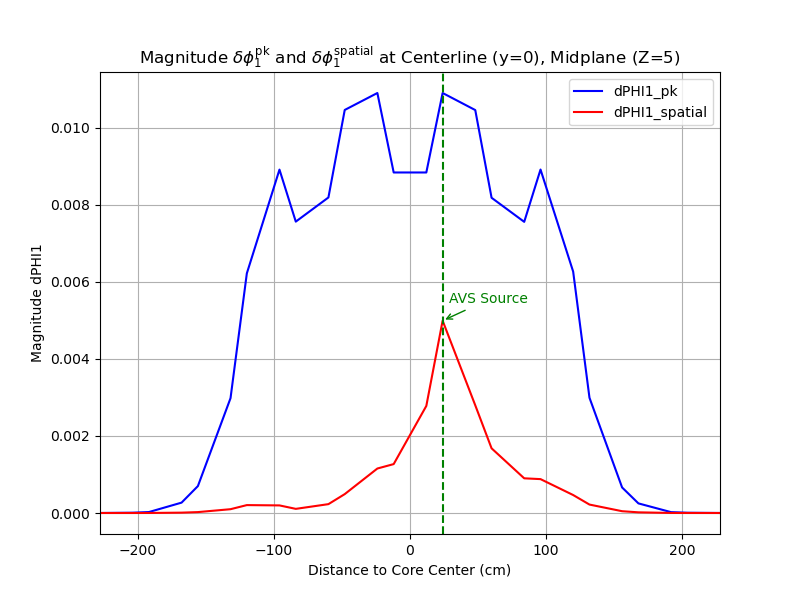
\includegraphics[width=\linewidth]{figures/Centerline_y0_OBJECTIVES3_TEST07_3DTriMG_HTTR_AVS_level1_dPHI_magnitude_G1.png}
        \end{subfigure}
        \hfill
        \begin{subfigure}{.48\textwidth}
          \centering
          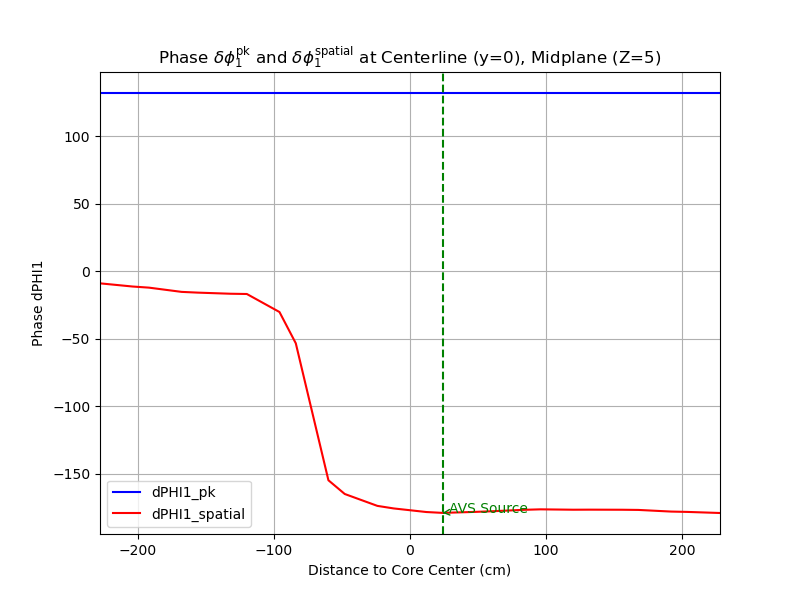
\includegraphics[width=\linewidth]{figures/Centerline_y0_OBJECTIVES3_TEST07_3DTriMG_HTTR_AVS_level1_dPHI_phase_G1.png}
        \end{subfigure}
        \caption{Magnitude (left) and phase (right) of the components of fast neutron noise for AVS in 3D HTTR at centerline ($y=0$), midplane ($Z=5$)}
        \label{fig:3DHTTRAVS_noise_component_results1}
\end{figure}
\begin{figure}[H]
        \centering
        \begin{subfigure}{.48\textwidth}
          \centering
          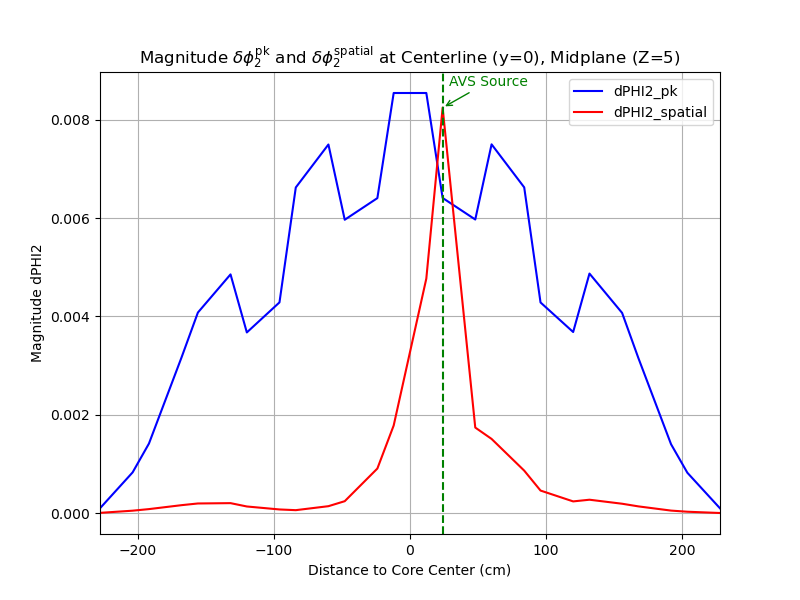
\includegraphics[width=\linewidth]{figures/Centerline_y0_OBJECTIVES3_TEST07_3DTriMG_HTTR_AVS_level1_dPHI_magnitude_G2.png}
        \end{subfigure}
        \hfill
        \begin{subfigure}{.48\textwidth}
          \centering
          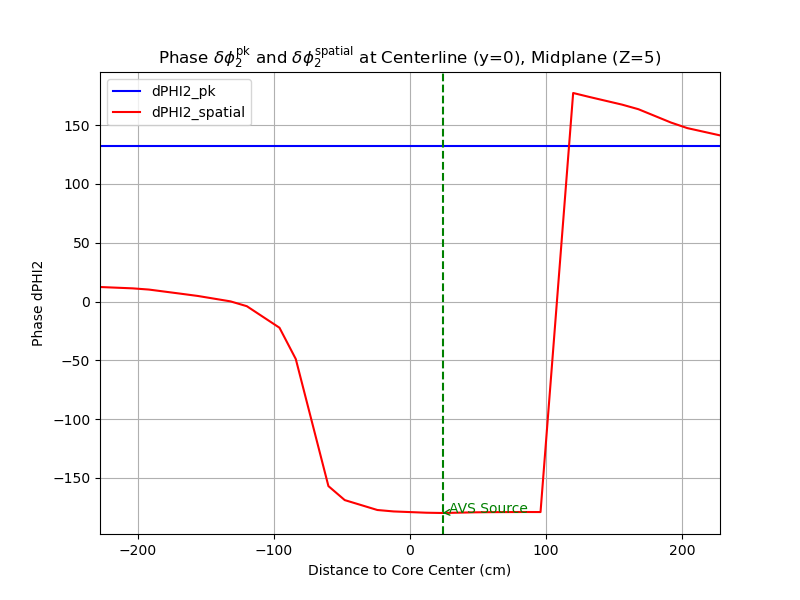
\includegraphics[width=\linewidth]{figures/Centerline_y0_OBJECTIVES3_TEST07_3DTriMG_HTTR_AVS_level1_dPHI_phase_G2.png}
        \end{subfigure}
        \caption{Magnitude (left) and phase (right) of the components of thermal neutron noise for AVS in 3D HTTR at centerline ($y=0$), midplane ($Z=5$)}
        \label{fig:3DHTTRAVS_noise_component_results2}
\end{figure}

Comparing Figure \ref{fig:3DHTTRAVS_noise_component_results1} and Figure \ref{fig:3DHTTRAVS_noise_component_results2}, we can see that in the fast group, the magnitude of the point kinetic component is more dominant compared to the spatial component. However, in the thermal group, the magnitude of the point kinetic component is lower at the AVS source location. This makes the contribution of the spatial component more apparent in the thermal group. The variation of the phase delay is mainly driven by the spatial components. It is expected that the point kinetic component will have no effect on the phase delays since it is a factor of the forward flux. Overall, we can see that the point kinetic component is more dominant in 3D HTTR compared to the spatial component, which means that the neutron noise is driven by the reactivity effect of the perturbation.

\subsection{3D HTTR with Fuel Assembly Vibration Source}

For the simulation of the fuel assembly vibration, the neutron noise source is modeled using the $\varepsilon/d$ method, similar to the 2D HTTR case. In this case, the frequency of vibration ($\omega_0$) is defined as 1 Hz, and the amplitude of vibration ($\varepsilon$) is 0.5 cm. Using this definition, the neutron noise source model is written as follows:
\begin{equation}
    \delta \Sigma_{a,g} (\textbf{r}_b, z ,\omega) = \left\{
\begin{array}{ll}
      -i \pi \varepsilon \Delta  \Sigma_{a,g} \delta (\omega - \omega_0) & \textbf{r}_b-\varepsilon\leq y \leq \textbf{r}_b + \varepsilon \\
      0 & \text{otherwise}\\
\end{array} 
\right. 
\end{equation}
This means that all the interfaces of the assembly become the source of neutron noise. The vibration is located at assembly number 65 along the $z$-axis, as shown in Figure \ref{fig:3DHTTRFAV}.
\begin{figure}[H]
        \centering
        \begin{subfigure}{.48\textwidth}
          \centering
          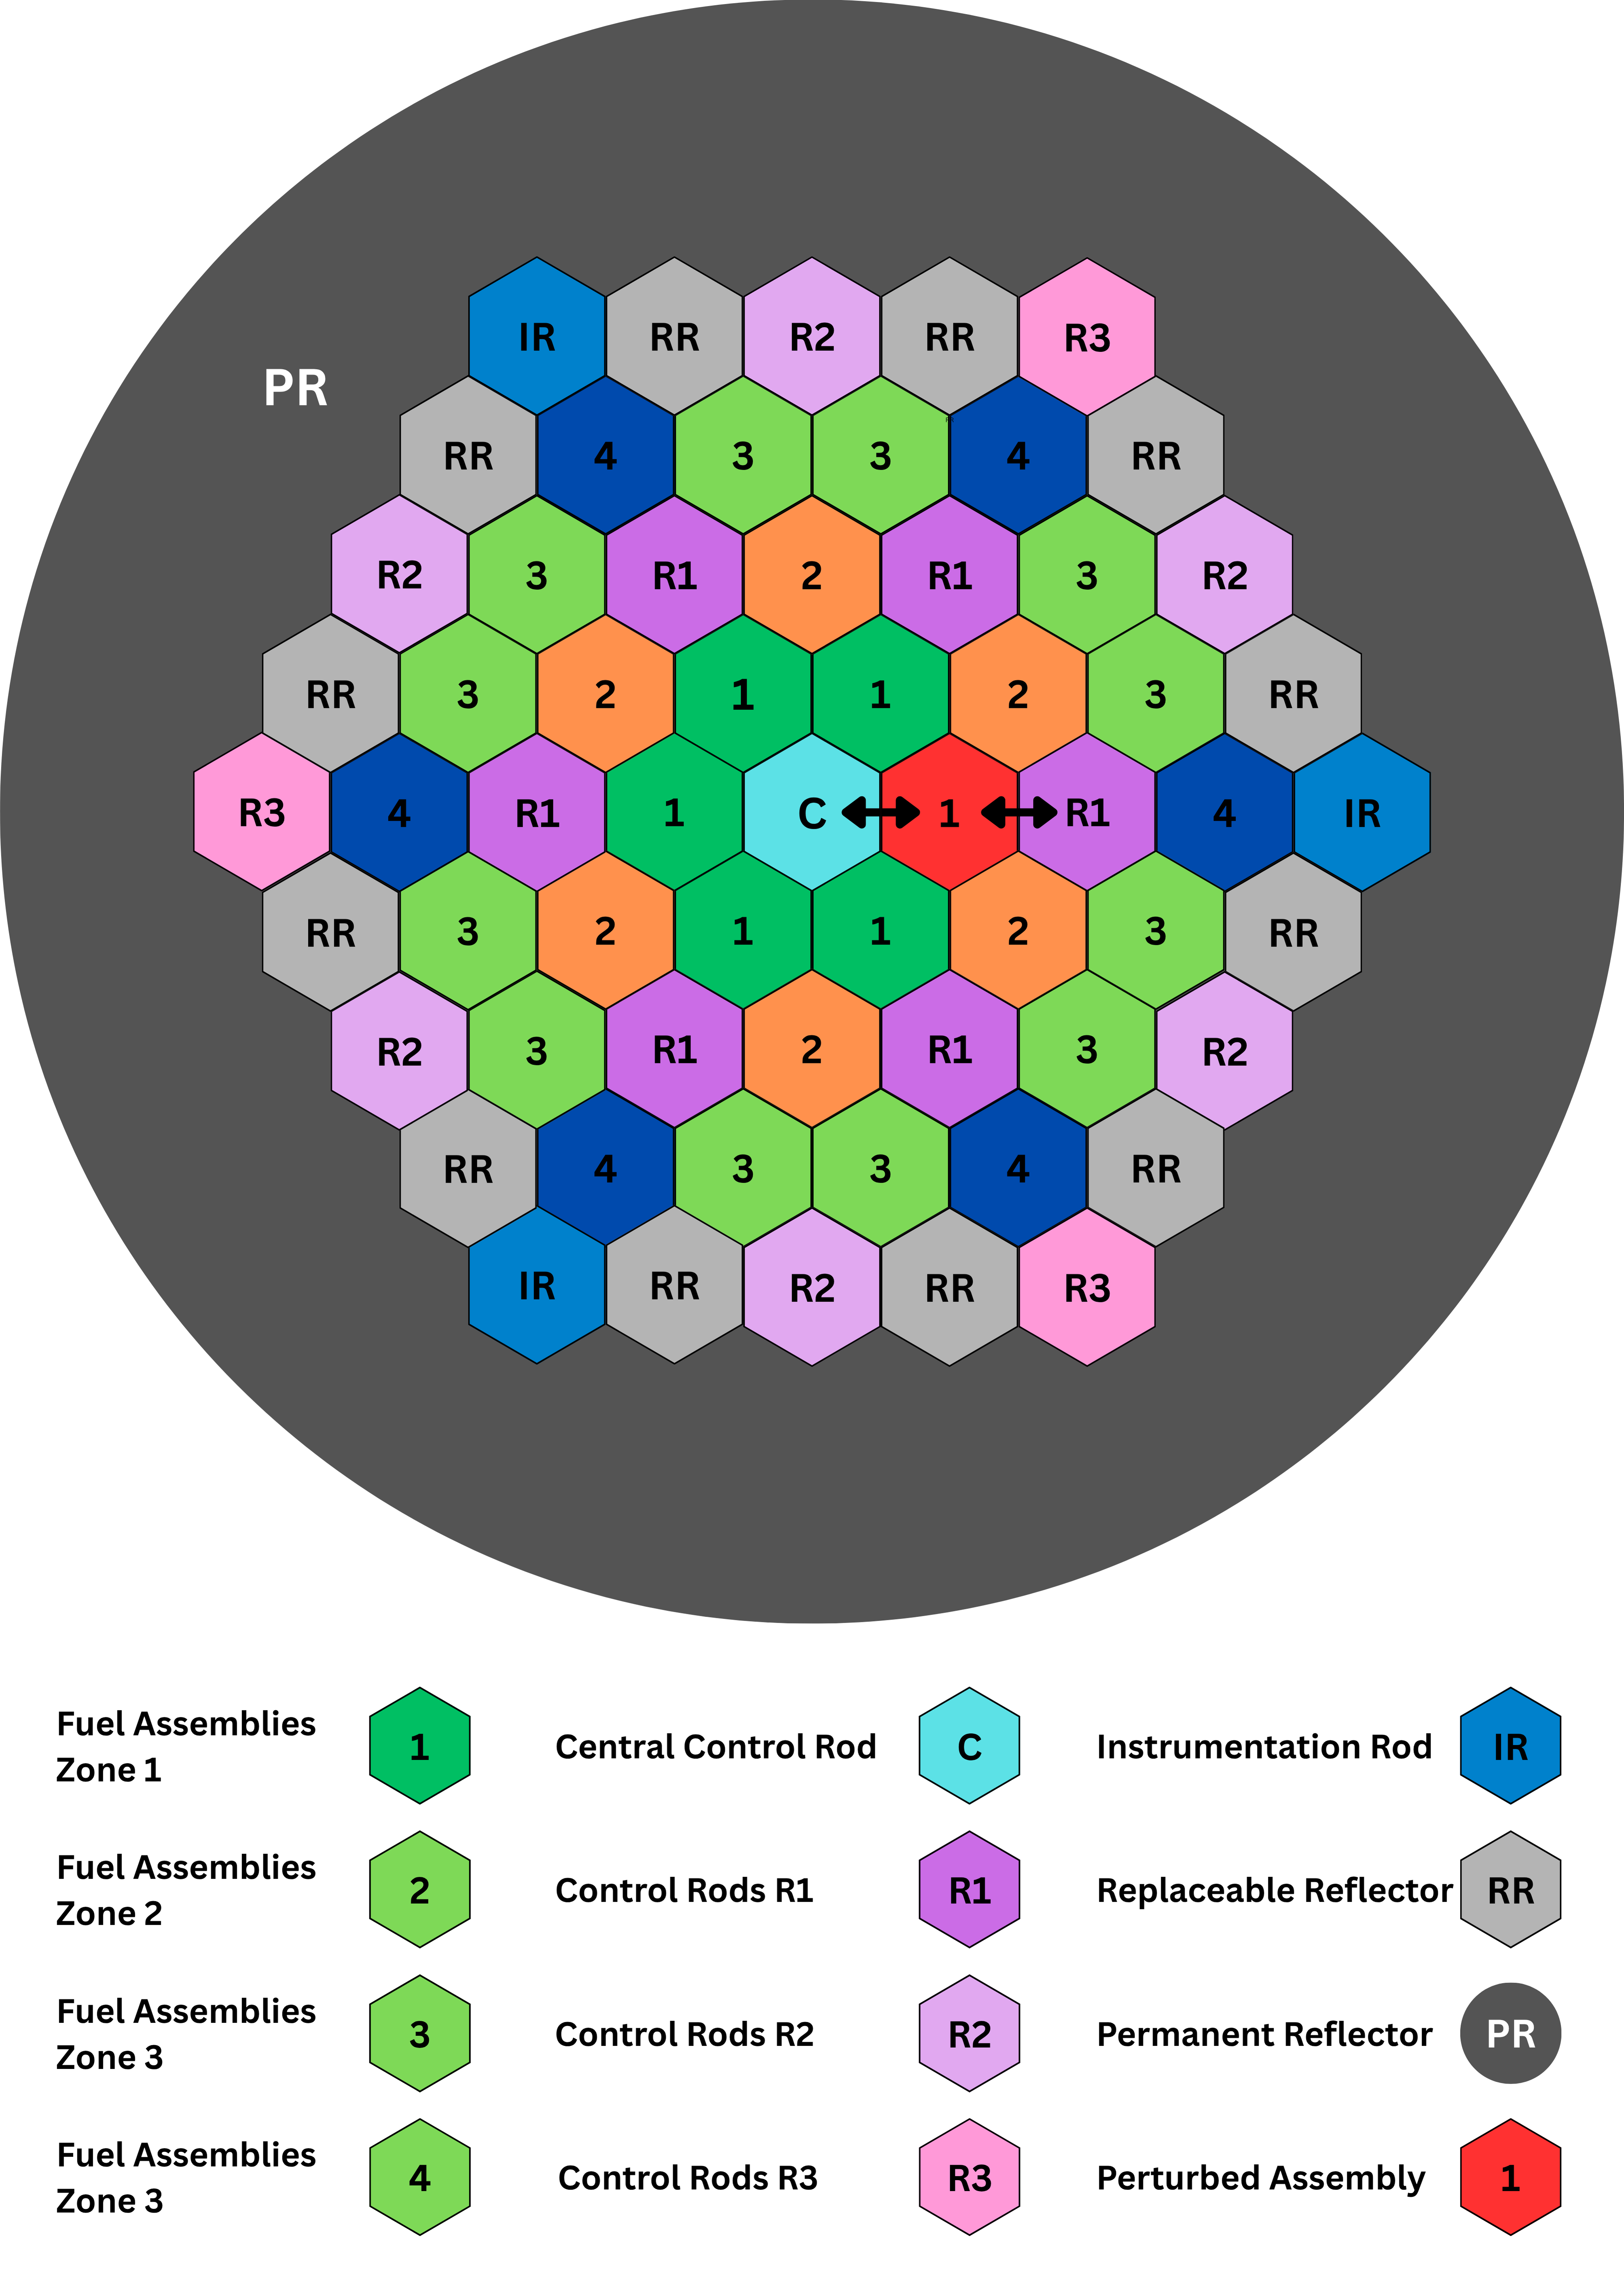
\includegraphics[width=\linewidth]{figures/HTTR3DFAV1.png}
        \end{subfigure}
        \hfill
        \begin{subfigure}{.48\textwidth}
          \centering
          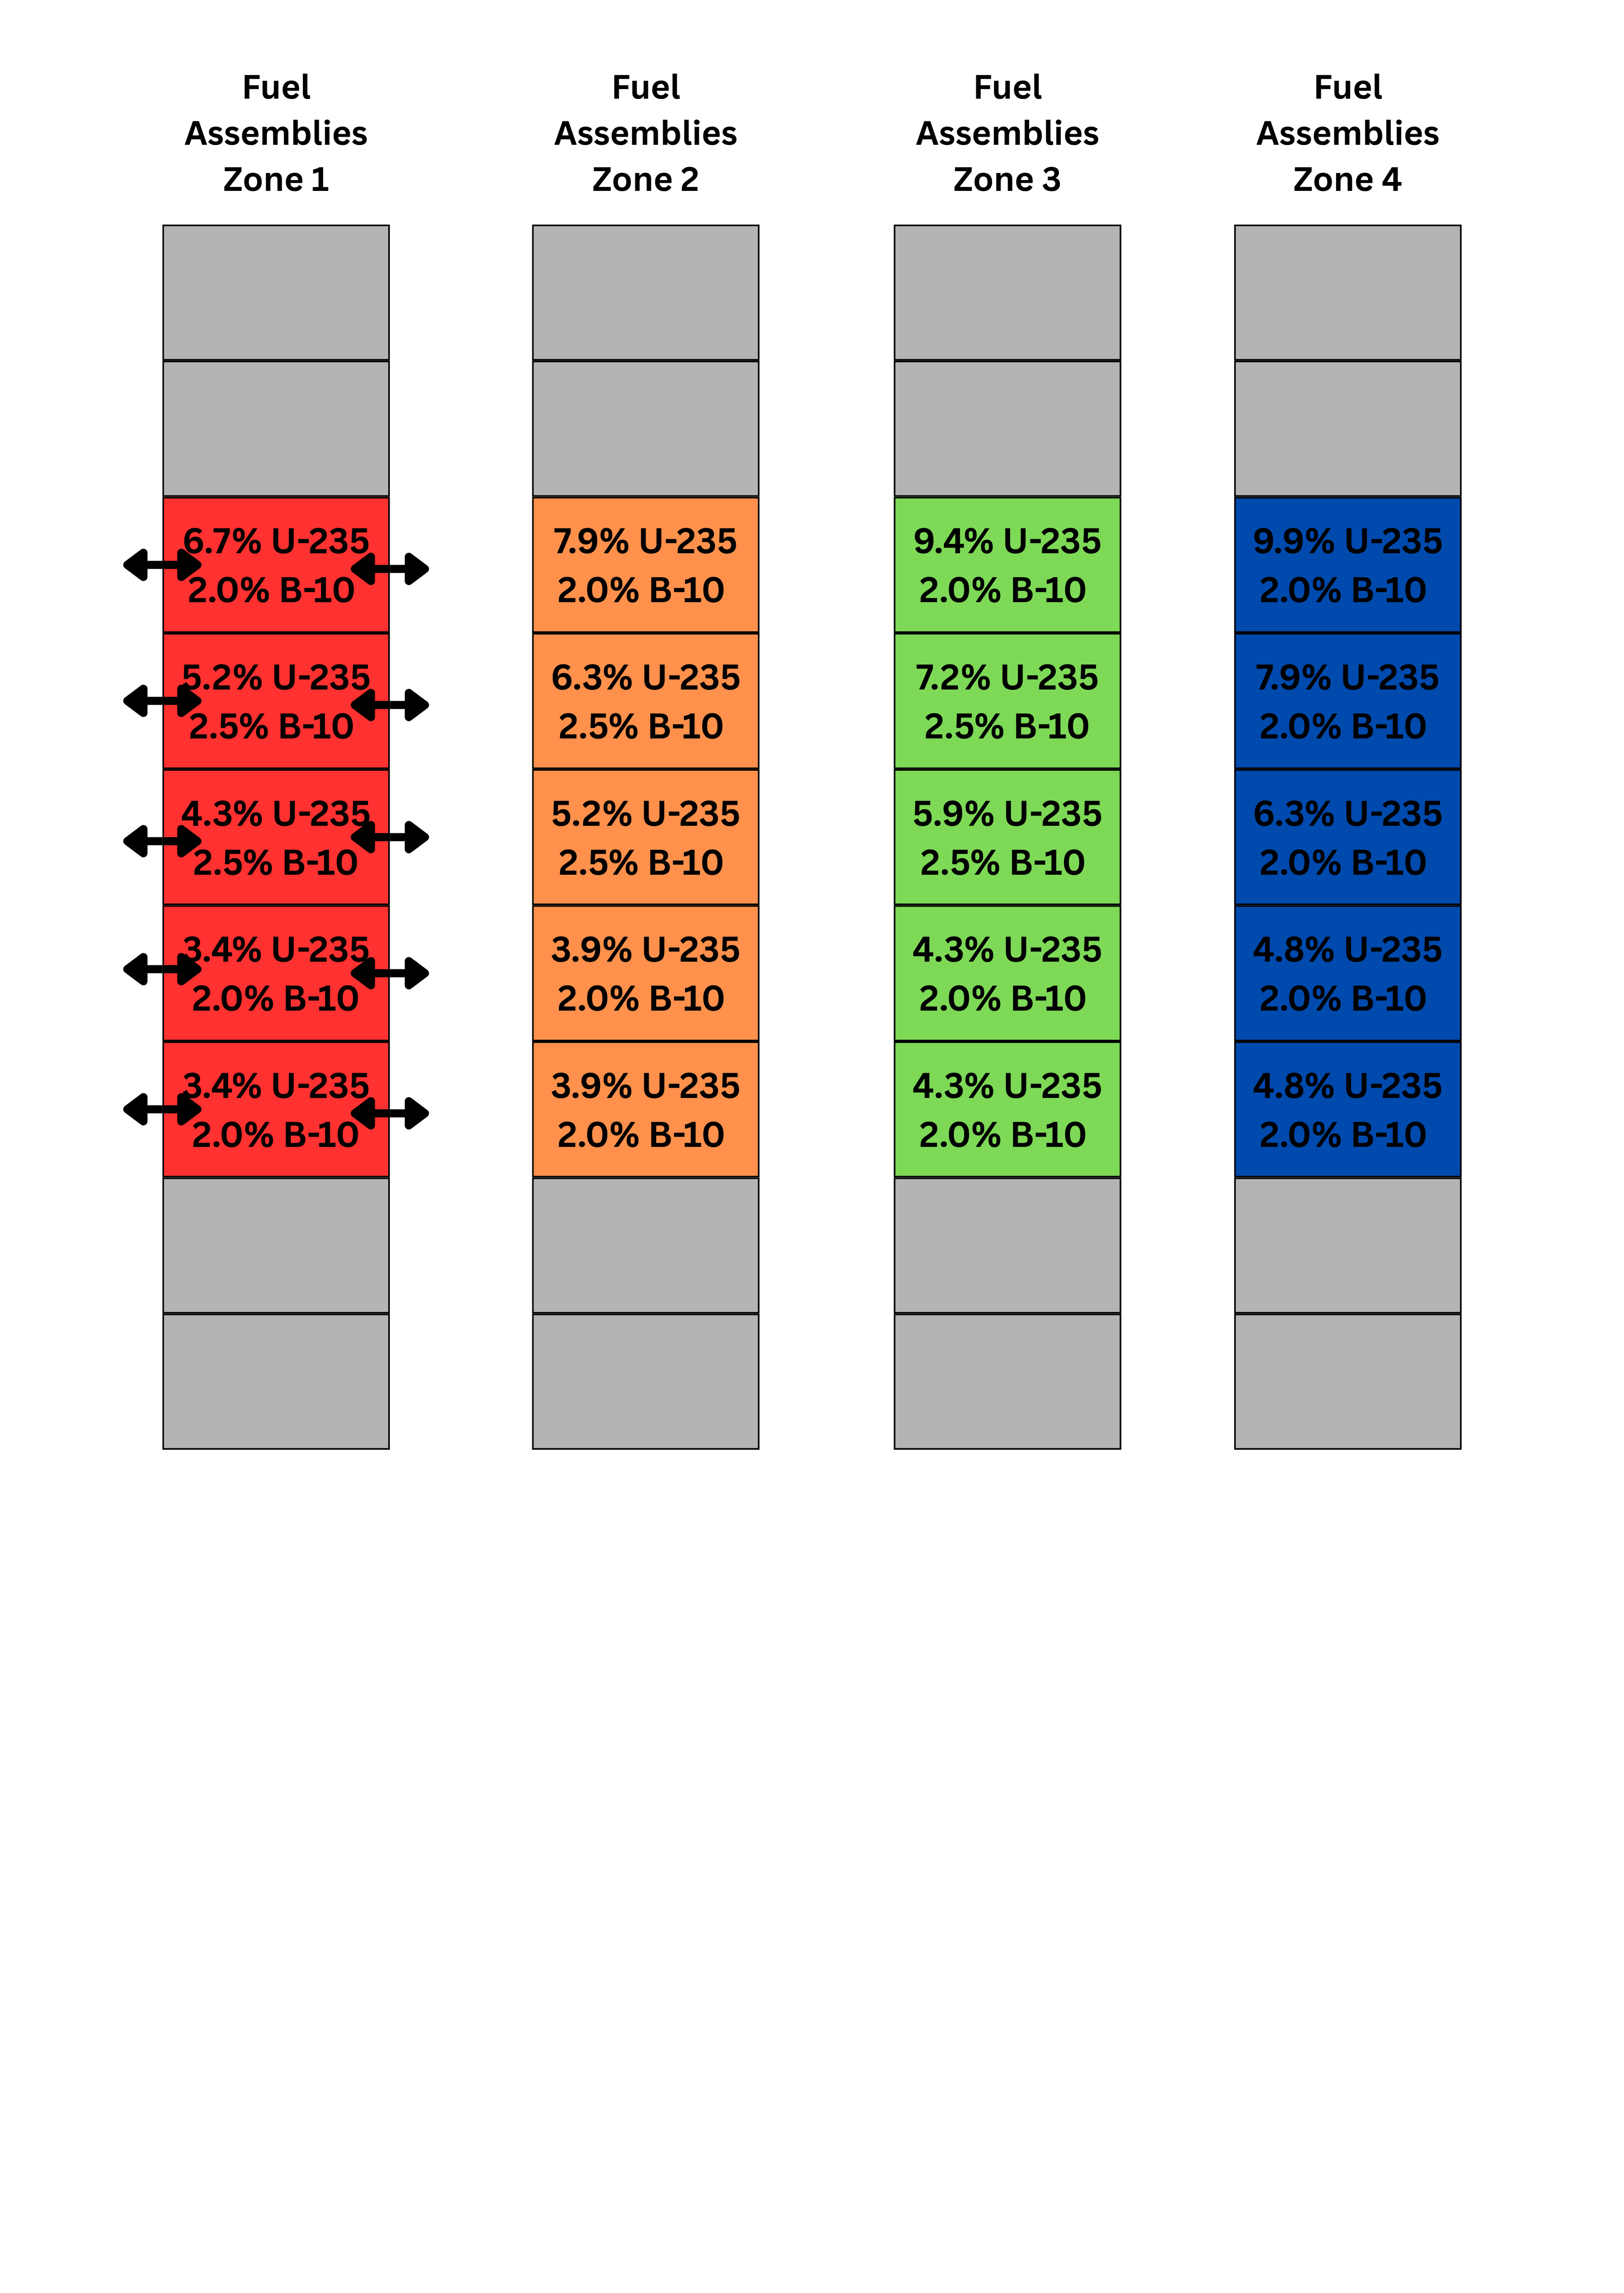
\includegraphics[width=\linewidth]{figures/HTTR3DFAV2.png}
        \end{subfigure}
        \caption{Location of the fuel assembly vibration for 3D HTTR}
        \label{fig:3DHTTRFAV}
\end{figure}

The results of the simulations are as follows:
\begin{figure}[H]
        \centering
        \begin{subfigure}{.48\textwidth}
          \centering
          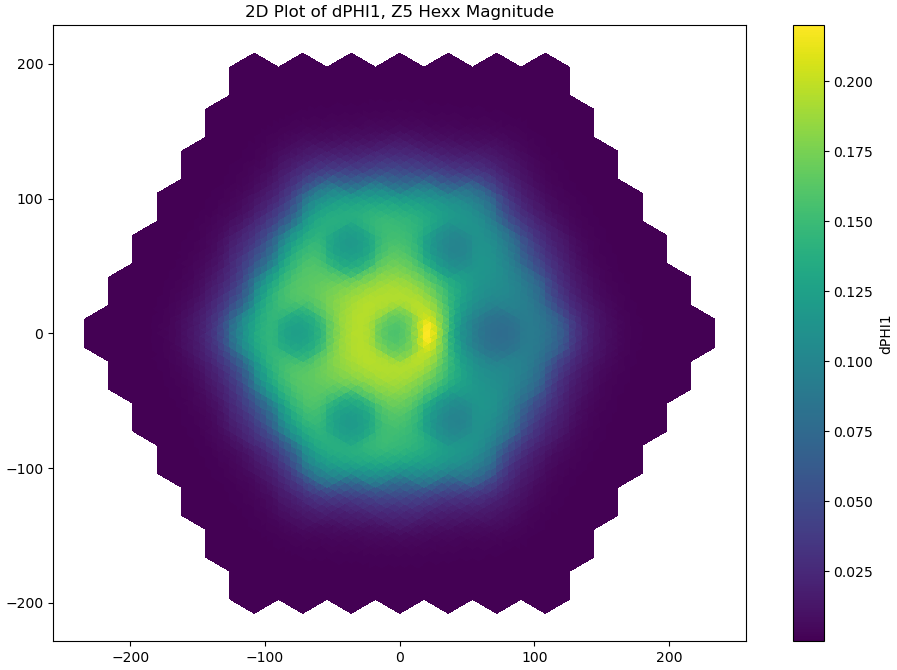
\includegraphics[width=\linewidth]{figures/OBJECTIVES3_TEST08_3DTriMG_HTTR_FAV_level3_NOISE_dPHI_magnitude_G1_Z5.png}
        \end{subfigure}
        \hfill
        \begin{subfigure}{.48\textwidth}
          \centering
          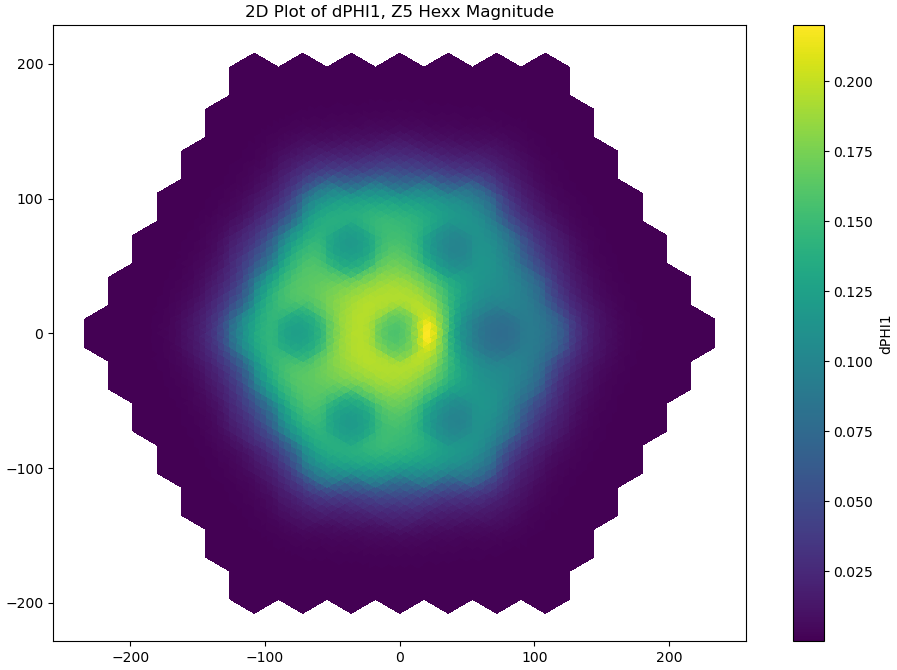
\includegraphics[width=\linewidth]{figures/OBJECTIVES3_TEST08_3DTriMG_HTTR_FAV_level3_NOISE_dPHI_magnitude_G1_Z5.png}
        \end{subfigure}
        \caption{Magnitude of the neutron noise for FAV in 3D HTTR at midplane ($Z = 5$)}
        \label{fig:3DHTTR_noise_FAV_results_mag}
\end{figure}
\begin{figure}[H]
        \centering
        \begin{subfigure}{.48\textwidth}
          \centering
          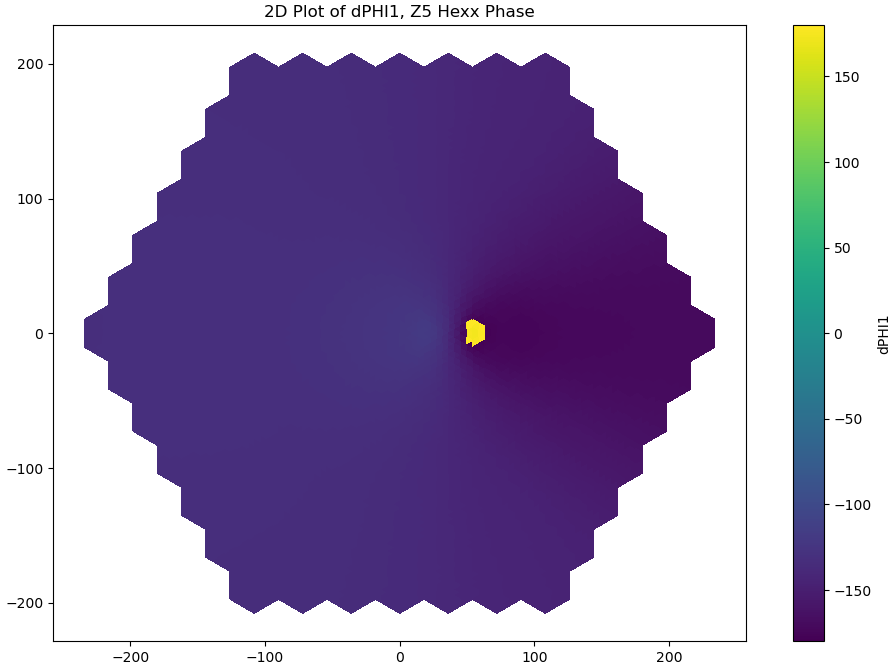
\includegraphics[width=\linewidth]{figures/OBJECTIVES3_TEST08_3DTriMG_HTTR_FAV_level3_NOISE_dPHI_phase_G1_Z5.png}
        \end{subfigure}
        \hfill
        \begin{subfigure}{.48\textwidth}
          \centering
          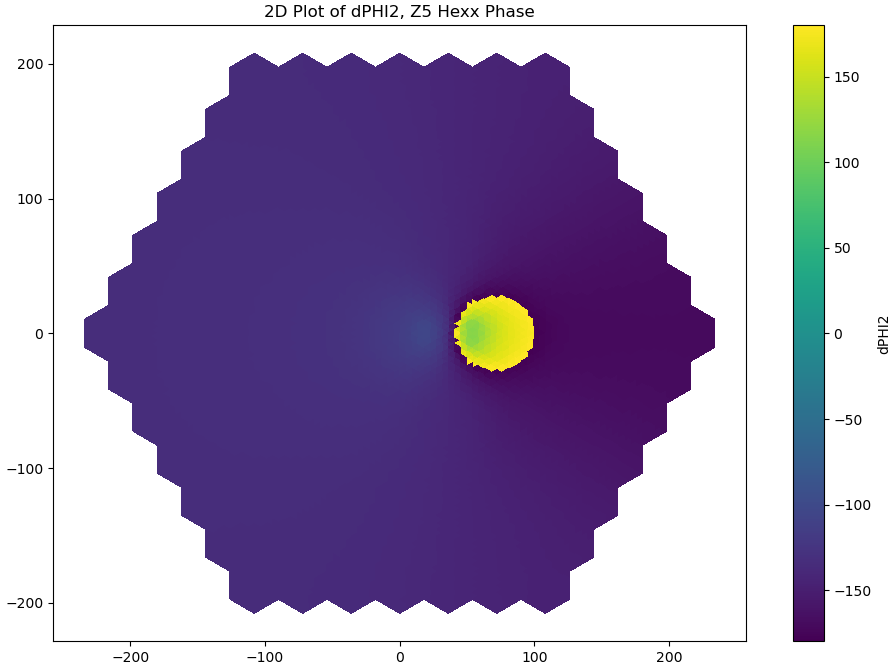
\includegraphics[width=\linewidth]{figures/OBJECTIVES3_TEST08_3DTriMG_HTTR_FAV_level3_NOISE_dPHI_phase_G2_Z5.png}
        \end{subfigure}
        \caption{Phase of the neutron noise for FAV in 3D HTTR at midplane ($Z = 5$)}
        \label{fig:3DHTTR_noise_FAV_results_phase}
\end{figure}

As seen in Figure \ref{fig:3DHTTR_noise_FAV_results_mag} and Figure \ref{fig:3DHTTR_noise_FAV_results_phase}, the neutron noise is more apparent in the thermal group and more dispersed in the fast group. This is a similar phenomenon compared to the FAV source in 2D HTTR. A similar opposing effect is expected in this case due to the out-of-phase neutron noise source model. Since the vibrating assembly is a fuel assembly, the opposing effect is not so apparent in the interfaces where the neighboring assembly is also a fuel assembly. This is expected since the difference between the macroscopic  cross-sections ($\Delta \Sigma_{a,g}$) is smaller at these interfaces. However, the opposing effect becomes more evident at the interfaces where the neighboring assembly is a reflector assembly. 

To further understand the driving force of neutron noise, we can split the neutron noise into its point kinetic component and its spatial component. Figures \ref{fig:3DHTTRFAV_noise_component_results1} and \ref{fig:3DHTTRFAV_noise_component_results2} show the point kinetic component and spatial component of the neutron noise in fast and thermal group with FAV source, taken at the centerline of the core ($y=0$) and midplane ($Z=5$).
\begin{figure}[H]
        \centering
        \begin{subfigure}{.48\textwidth}
          \centering
          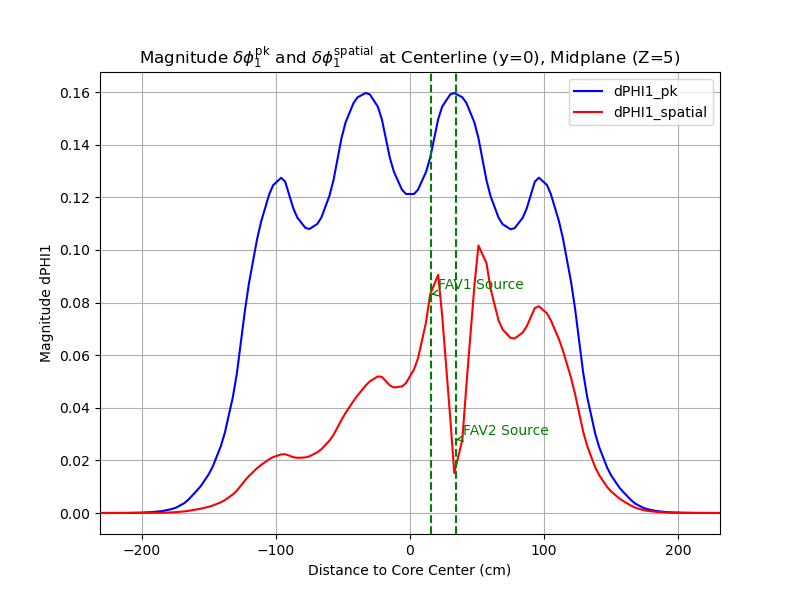
\includegraphics[width=\linewidth]{figures/Centerline_y0_OBJECTIVES3_TEST08_3DTriMG_HTTR_FAV_level3_dPHI_magnitude_G1.png}
        \end{subfigure}
        \hfill
        \begin{subfigure}{.48\textwidth}
          \centering
          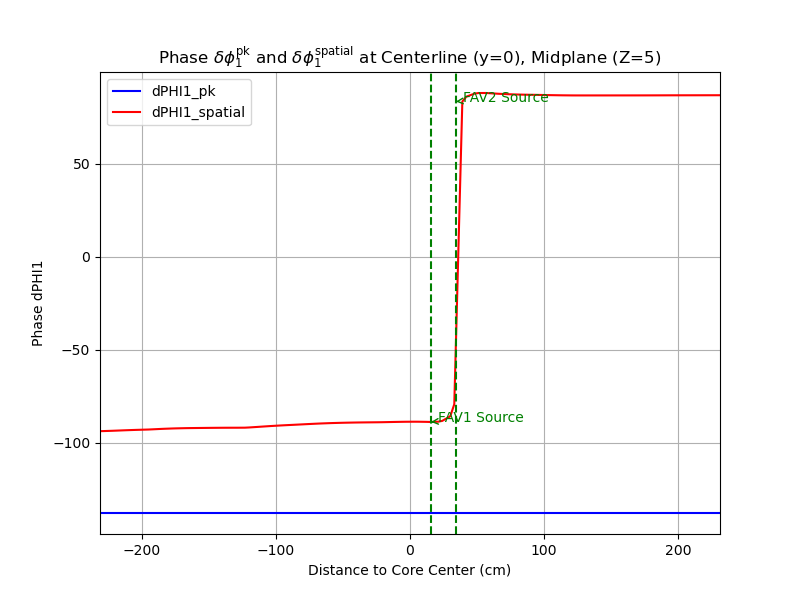
\includegraphics[width=\linewidth]{figures/Centerline_y0_OBJECTIVES3_TEST08_3DTriMG_HTTR_FAV_level3_dPHI_phase_G1.png}
        \end{subfigure}
        \caption{Magnitude (left) and phase (right) of the components of fast neutron noise for FAV in 3D HTTR at centerline ($y=0$), midplane ($z=5$)}
        \label{fig:3DHTTRFAV_noise_component_results1}
\end{figure}
\begin{figure}[H]
        \centering
        \begin{subfigure}{.48\textwidth}
          \centering
          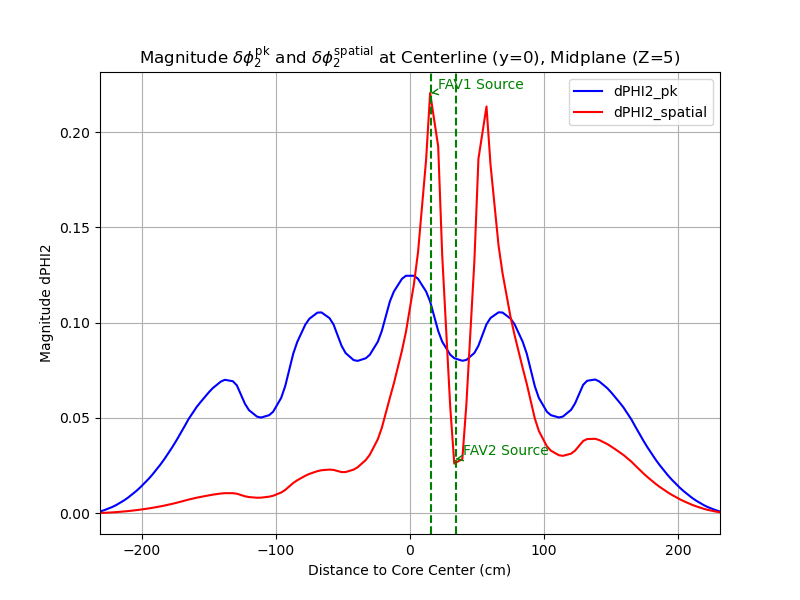
\includegraphics[width=\linewidth]{figures/Centerline_y0_OBJECTIVES3_TEST08_3DTriMG_HTTR_FAV_level3_dPHI_magnitude_G2.png}
        \end{subfigure}
        \hfill
        \begin{subfigure}{.48\textwidth}
          \centering
          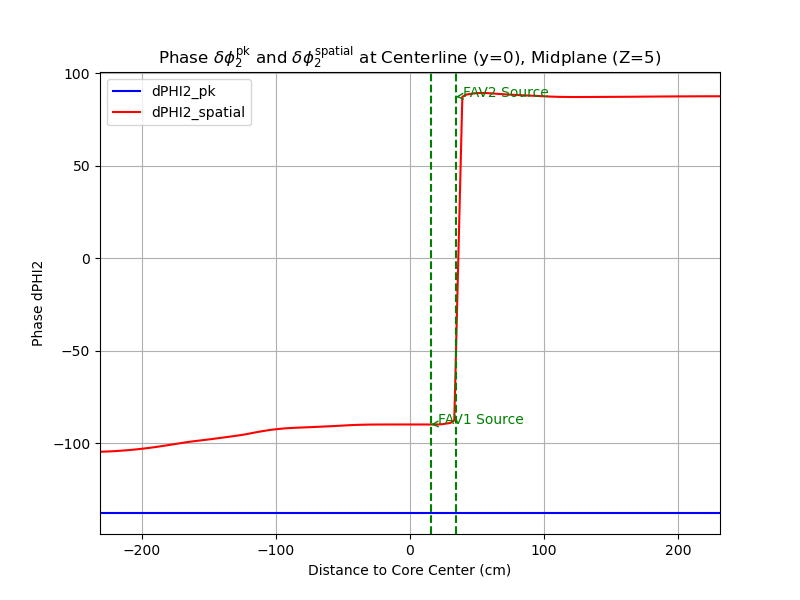
\includegraphics[width=\linewidth]{figures/Centerline_y0_OBJECTIVES3_TEST08_3DTriMG_HTTR_FAV_level3_dPHI_phase_G2.png}
        \end{subfigure}
        \caption{Magnitude (left) and phase (right) of the components of thermal neutron noise for FAV in 3D HTTR at centerline ($y=0$), midplane ($z=5$)}
        \label{fig:3DHTTRFAV_noise_component_results2}
\end{figure}

Comparing Figure \ref{fig:3DHTTRFAV_noise_component_results1} and Figure \ref{fig:3DHTTRFAV_noise_component_results2}, we see that the spatial component in the fast group has more influence than in the other cases. The point kinetic component remains dominant in this case, resulting in a more dispersed magnitude of neutron noise in the fast group. In the thermal group, we can see that the spatial component dominates the magnitude of the neutron noise. Similar to the 3D HTTR AVS case, the spatial component influences the phase delays similarly to the AVS source. Out-of-phase delays are more apparent compared to other cases. In general, we can see that the point kinetic component and the spatial component have different effects on the magnitude of neutron noise, while the phase of the neutron noise is mainly affected by the spatial component of the neutron noise. 

\section{Comparison of Noise Responses Between HTTR and LWR}

\subsection{2D Neutron Noise Responses}

For the comparison in 2D, the ZPRTF from 2D HTTR is compared with the ZPRTF from 2D C3 Benchmark, 2D BIBLIS Benchmark, and 2D VVER-400. The neutron noise simulation of 2D C3 Benchmark, 2D VVER-400 and 2D BIBLIS Benchmark will be shown in Appendix \ref{ch:appendixA}.

This comparison is done by performing 100 simulations for each 2D cases with variable frequencies, ranging from $10^{-4}$ Hz to $10^{4}$ Hz. The results of ZPRTF are shown in Figure \ref{fig:2DTransferFunction}.
\begin{figure}[H]
        \centering
        \begin{subfigure}{.48\textwidth}
          \centering
          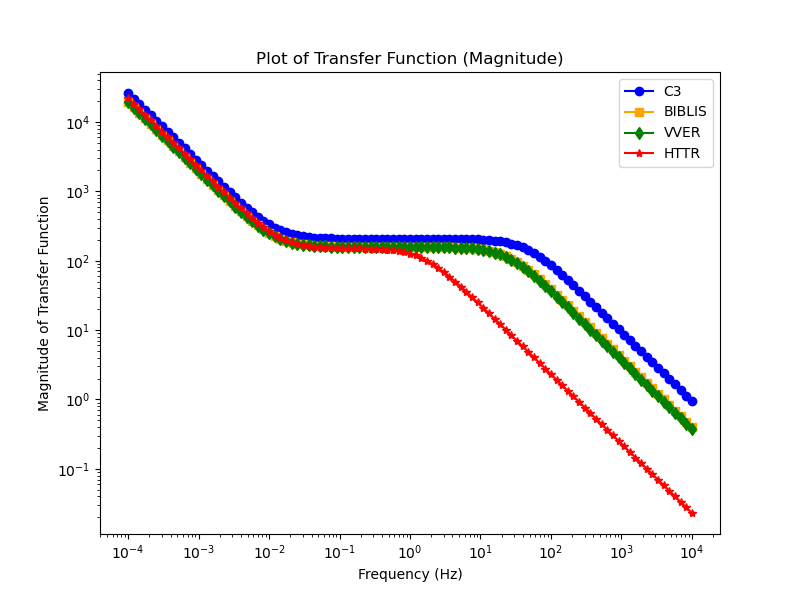
\includegraphics[width=\linewidth]{figures/Transfer_Function_2D_Comparison_Magnitude.png}
        \end{subfigure}
        \hfill
        \begin{subfigure}{.48\textwidth}
          \centering
          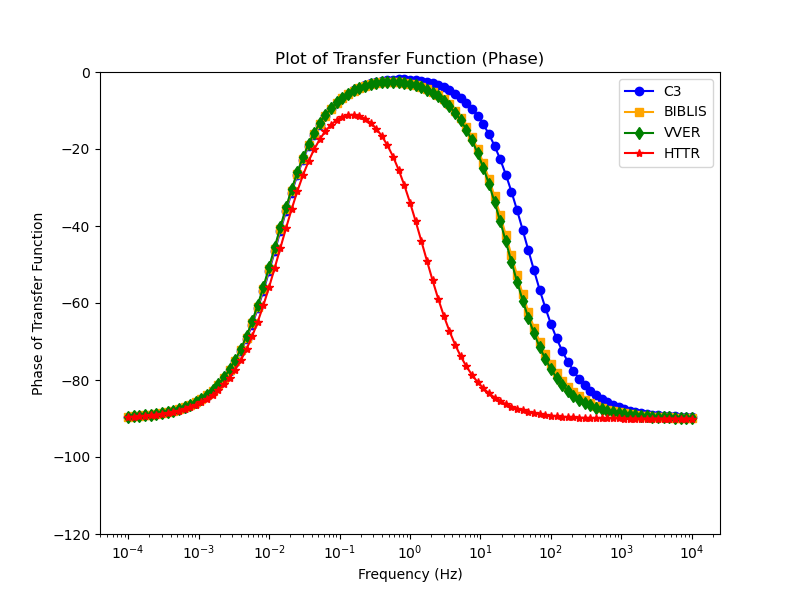
\includegraphics[width=\linewidth]{figures/Transfer_Function_2D_Comparison_Phase.png}
        \end{subfigure}
        \caption{Magnitude (left) and phase delay (right) of transfer function in 2D HTTR}
        \label{fig:2DTransferFunction}
\end{figure}

As seen in Figure \ref{fig:2DTransferFunction}, the ZPRTF of 2D HTTR generally follows the expected behavior of the ZPRTF. At lower and higher frequencies, the transfer function generally follows the $1/\omega$ behavior, which is expected in the ZPRTF. However, we can see that the 2D HTTR has a narrower plateau compared to other transfer functions. In the phase delay plot, we can see that the peak of 2D HTTR ZPRTF is further away from zero compared to other transfer functions. The HTTR ZPRTF deviates at around 1 Hz to 50 Hz. This means that within these frequencies, the spatial component of neutron noise in HTTR will have more significant effect compared to LWRs at the same range of frequencies.

\subsection{3D Neutron Noise Responses}

For the comparison in 3D, the ZPRTF from 3D HTTR is compared with the ZPRTF from 3D Westinghouse 4-loop PWR , 3D Langenbuch (LMW) Benchmark, and 3D VVER-400. The neutron noise simulation of 3D Westinghouse 4-loop PWR, 3D Langenbuch (LMW) Benchmark, and 3D VVER-400 will be shown in Appendix \ref{ch:appendixA}.

Similar to the 2D case, this comparison is done by performing 100 simulations for each 3D cases with variable frequencies, ranging from $10^{-4}$ Hz to $10^{4}$ Hz. The results of ZPRTF are shown in Figure \ref{fig:3DTransferFunction}.
\begin{figure}[H]
        \centering
        \begin{subfigure}{.48\textwidth}
          \centering
          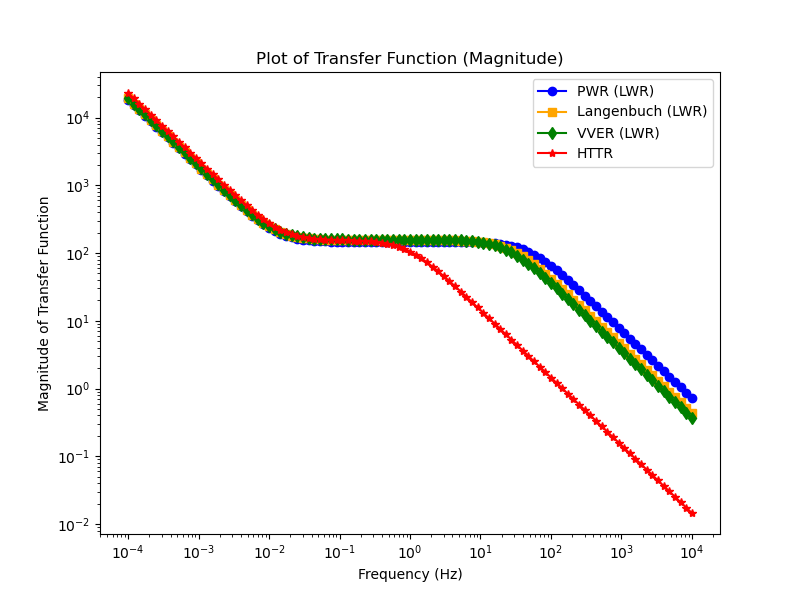
\includegraphics[width=\linewidth]{figures/Transfer_Function_3D_Comparison_Magnitude.png}
        \end{subfigure}
        \hfill
        \begin{subfigure}{.48\textwidth}
          \centering
          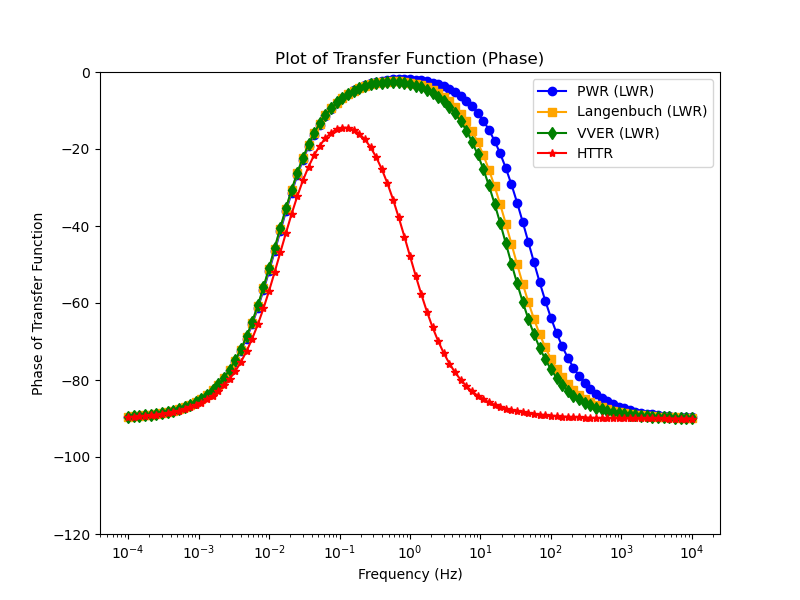
\includegraphics[width=\linewidth]{figures/Transfer_Function_3D_Comparison_Phase.png}
        \end{subfigure}
        \caption{Magnitude (left) and phase delay (right) of transfer function in 3D HTTR}
        \label{fig:3DTransferFunction}
\end{figure}

As seen in Figure \ref{fig:3DTransferFunction}, the ZPRTF of 3D HTTR generally follows the expected behavior of the ZPRTF, as expected. At lower and higher frequencies, the transfer function generally follows the $1/\omega$ behavior. Similar to the 2D HTTR case, we also see that the 3D HTTR has a shorter plateau compared to other transfer functions. In the phase delay plot, we can see that the peak of 3D HTTR ZPRTF is further away from zero compared to other transfer functions. The HTTR ZPRTF deviates at around 1 Hz to 50 Hz. Similar to the 2D HTTR case, this means that within these frequencies, the spatial component of neutron noise in HTTR will have more significant effect compared to LWRs at the same range of frequencies.

\section{Conclusion}

In this chapter, neutron noise simulations of 2D and 3D HTTR have been performed using two different noise sources for each geometry: the absorber of variable strength and the fuel assembly vibration.

For the absorber of variable strength source, both 2D and 3D HTTR simulations show that the neutron noise is more localized in the thermal group and more dispersed in the fast group. This is likely due to the larger mean free path of neutrons in the fast group. It is also observed that the point kinetic component of the neutron noise is more dominant than the spatial component of neutron noise. For the fuel assembly vibration case, a similar localized effect is observed in the thermal group. Additionally, the 2D and 3D HTTR FAV results show that the spatial component of the neutron noise has significant effect on the overall effect of neutron noise. This is more apparent when the neighboring assembly of the vibrating has a different characteristic (e.g., the neighboring assembly of the fuel assembly is a reflector assembly). Overall, the results show that the point kinetic component of neutron noise is more dominant than the spatial component in HTTR. This shows that the neutron noise is largely driven by the reactivity effect of the perturbation.

The ZPRTF of 2D and 3D HTTR was also compared with LWRs. The results show that HTTR generally follows the expected behavior of ZPRTF. The uniqueness of HTTR lies in the fact that it has a narrower plateau compared to LWRs. This means that at around 1 Hz to 50 Hz, the spatial component of neutron noise in HTTR will have more significant effect compared to LWRs. Overall, the simulations show that HTTR follows the expected behavior of neutron noise. Thus, neutron noise analysis can be used to detect anomalies in HTTR.